\documentclass[12pt, a4paper, onecolumn]{article}
\usepackage{fontspec}
\usepackage{titlesec}
\usepackage{tocloft}
\usepackage[english]{babel}
\usepackage{blindtext}
\usepackage{subfig}
\usepackage{pgf}
\setmainfont{Georgia}
\usepackage{parskip}
\usepackage{float}
\usepackage{multicol}


\newcommand\sectionfont{\normalfont\fontspec{Arial}\fontsize{14pt}{0}\bfseries}
\newcommand\subsectionfont{\normalfont\fontspec{Arial}\fontsize{13pt}{0}\bfseries}
\newcommand\subsubsectionfont{\normalfont\fontspec{Arial}\fontsize{12pt}{0}\bfseries}
\newcommand\tocsectionfont{\normalfont\fontspec{Arial}\fontsize{12pt}{0}\bfseries}
\newcommand\tocsubsectionfont{\normalfont\fontspec{Arial}\fontsize{11pt}{0}\bfseries}
\newcommand\tocsubsubsectionfont{\normalfont\fontspec{Arial}\fontsize{11pt}{0}}
\newcommand\toctitlefont{\normalfont\fontspec{Arial}\fontsize{16pt}{0}\bfseries}

\titleformat{\section}{\sectionfont}{\thesection}{20pt}{}
\titleformat{\subsection}{\subsectionfont}{\thesubsection}{20pt}{}
\titleformat{\subsubsection}{\subsubsectionfont}{\thesubsubsection}{20pt}{}

\renewcommand{\cftsecfont}{\tocsectionfont}
\renewcommand{\cftsubsecfont}{\tocsubsectionfont}
\renewcommand{\cftsubsubsecfont}{\tocsubsubsectionfont}
\renewcommand{\cftsecpagefont}{\tocsectionfont}
\renewcommand{\cftsubsecpagefont}{\tocsubsectionfont}
\renewcommand{\cftsubsubsecpagefont}{\tocsubsubsectionfont}
\renewcommand{\cfttoctitlefont}{\toctitlefont}

\newcommand{\parag}[1]{
	\textbf{#1} \hspace{0pt} \\
}

\addto\captionsenglish{
	\renewcommand{\contentsname}{Table of Contents}
}

\begin{document}
	
	\title{Fall detection using smart phone application}
	\maketitle

	\tableofcontents
	\newpage
	
	\section{Introduction}
	
	Accidents related to falling is a major issue in our society. In fact, according to the World Health Organization, "Falls are the second leading cause of accidental or unintentional injury deaths worldwide" \cite{who}. Globally, an average of 37.3 million people (Jan 2018) suffer from injuries related to a fall each year, which are severe enough to seek medical attention. Out of these, no less than an estimated 640 000 individuals die as a direct consequence of the fall \cite{who}. Fall  related accidents are therefore to be considered as a significant world wide health problem. 
	
	Although age is identified as a key driving factor behind fall related injuries, it is not by far the only reason that people hurt themselves this way every year.  Other risk factors include 
	\begin{itemize}
		\item Occupations which require you to work at an elevated height.
		\item Alcohol and substance abuse.
		\item Medical conditions contributing to a reduced sense of balance or vision.
		\item Sporting.	
	\end{itemize}
	
	In Sweden alone, statistics shows even darker figures. Here, falling is the single one reason responsible for the greatest number of accident related fatalities, hospitalizations, and visits to emergency clinics, outnumbering traffic accidents, who come in second \cite[p~3,5]{msb_report}. On top of that, in Sweden, falling is together with poisoning, the type of accident who poses the biggest annual growth, having duplicated the amount of yearly incidents since 2000 \cite{soc_olyckor}. Studies have also shown that peoples perception target traffic accidents as the the most common cause of the above \cite[p~5]{msb_report}. That is however not true, but a reasonable explanation for this is according to MSB (Swedish Civil Contingencies Agency) that most fall related accidents happen in a domestic area and are thus not as dramatic as a car accident or a fire for example. This tend to give this type of accident less space in the common media. 
	
		\subsection{Background}
		
		Work environments are a common ground for falling accidents. The work force in Sweden is by no means an exception to this. The swedish work environment authority (Arbetsmiljöverket) published a study in 2016, claiming that fall accidents are the most versus second most common reason for absence in work due to accident, for women and men respectively \cite[p~1]{av}. This does not only have an impact on the lives of the individual and his or her family, it also poses serious economical damage to the society in general, and the affected organizations in particular. The diagrams shown in figure \ref{fig:Men-Women-Falling-From-Same-Ellevation} and \ref{fig:Men-And-Women-Falling-Form-Elevated-height} illustrates the amount of reported fall related accidents per 1000 employed men and women respectively, in the most affected occupations . 
		
		\begin{figure}[h]
			\centering
			\subfloat{{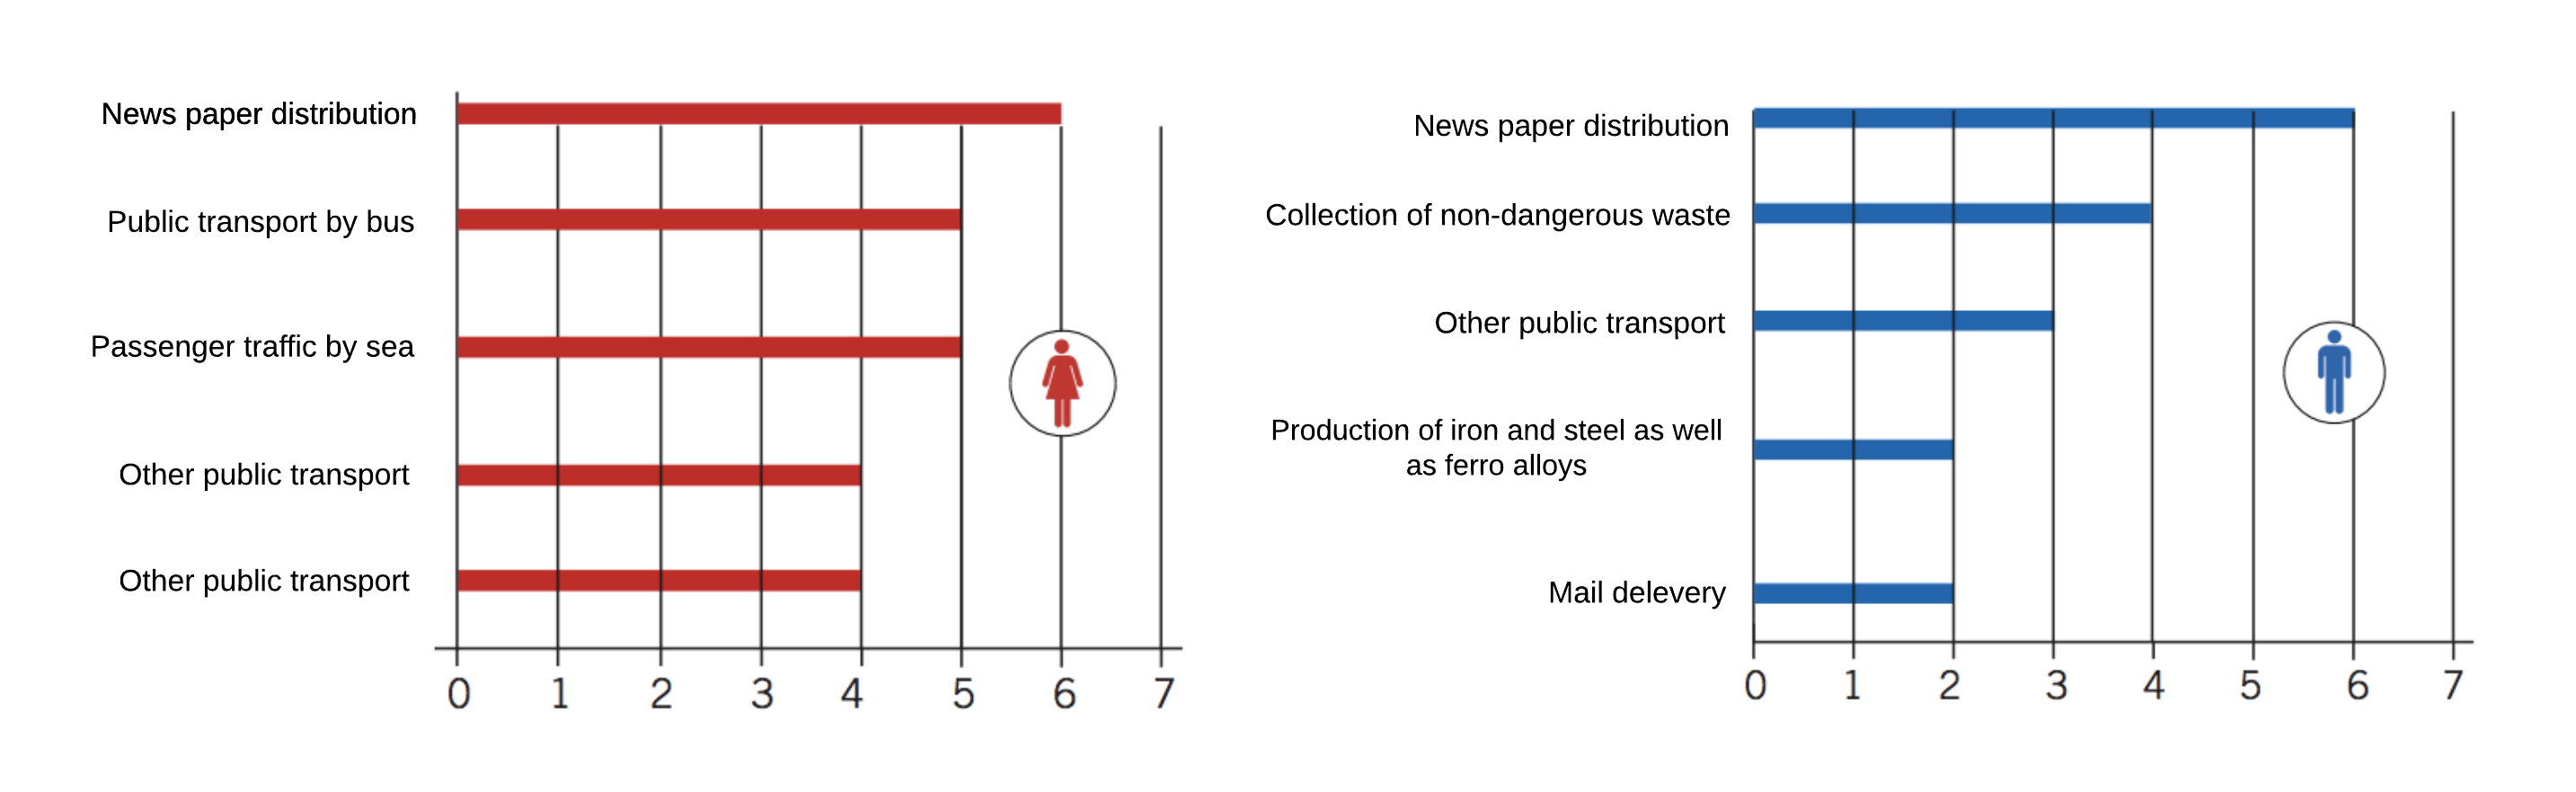
\includegraphics[width=14cm]{../img/Fall_from_ground_women_and_men.png} }}%
			\qquad

			\caption{Work areas with most reported fall accidents from standing level. Amount per 1000 employed women and men respectively}%
			\label{fig:Men-Women-Falling-From-Same-Ellevation}%
		\end{figure}
		
		\begin{figure}[h]
			\centering
			\subfloat{{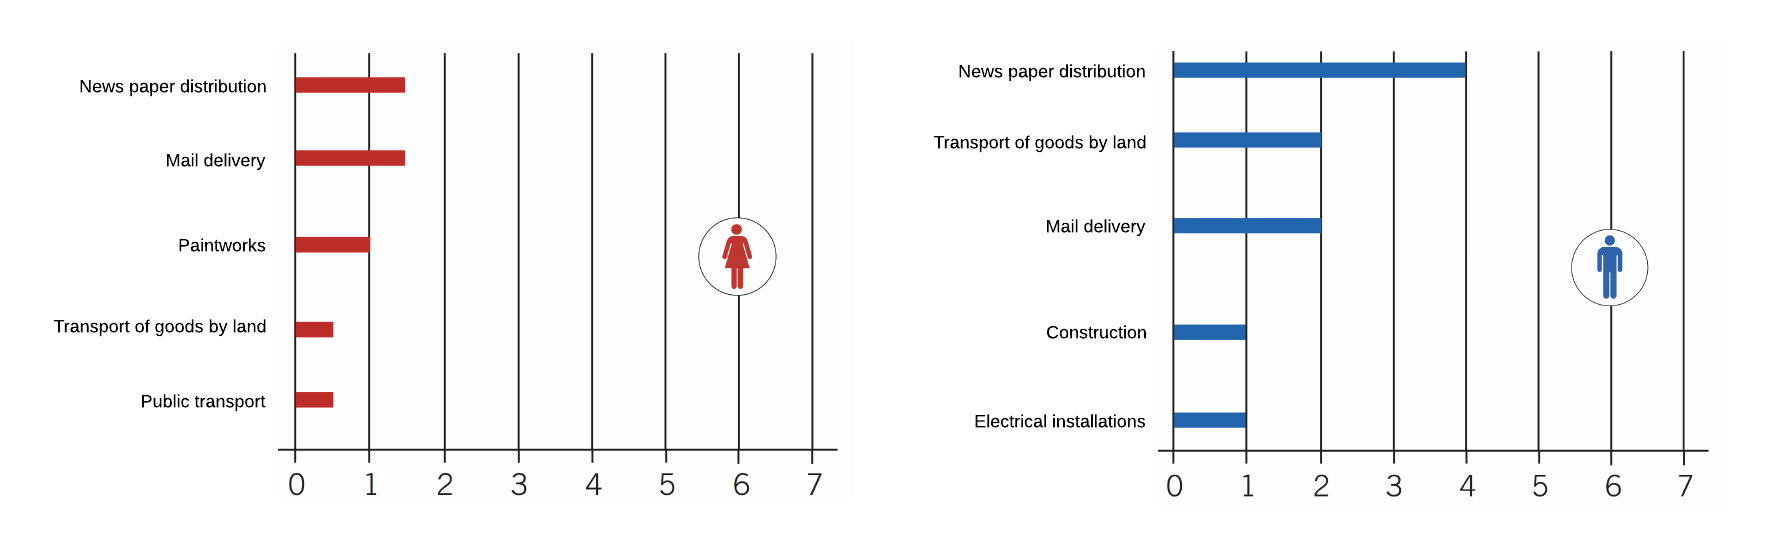
\includegraphics[width=14cm]{../img/Falls_from_elevated_height_men_and_women.png} }}%
			\qquad
			\caption{Work areas with most reported fall accidents from elevated level. Amount per 1000 employed women and men respectively}%
			\label{fig:Men-And-Women-Falling-Form-Elevated-height}%
		\end{figure}
	
			In relation to the above statistics, minimizing the duration between the occurrence of the fall accident and treatment can in some cases be imperative. This is especially the case where significant trauma to the head is present. In such cases, the sooner an injured person gets treatment, the better the odds of recovering. In cases where a fall accident is occurring in the presence of others, reporting the accident to a medical professional might often be a quick task. However, many fall accidents occur without any other human being around to detect it. In such cases, and especially if the victim is unconscious, alerting medical staff might not be possible.
		
		
		\subsection{Problem}
		
		Falling accidents are common, and it is important that a person who suffers an accident, is aided as quickly as possible to minimize the consequences of the accident. Since a person who suffers a fall may end up in a situation where the person is unable to call for help, for example, because the person is injured or unconscious, an application that could send an automatic alarm could be of great use. An automatic alarm would help minimize the time between the accident and help arriving. Without the alarm, it could take a long time before the person is found by passers-by. For this reason, we want to investigate the possibility of creating a mobile application that can detect falling accidents and report to registered contacts. A mobile application has the advantage that most people already have a smart phone, so if a mobile application could accomplish the task successfully, the cost would be minimized since there will be no need for additional hardware.
		
		This leads us to wonder if it is possible to create such an application. It may be difficult to achieve accuracy in fall detection using only the sensors in the mobile phones that exists on the market today. And if falls were successfully detected, would it be possible to filter out other activities in daily life that resembles falls such as running, jumping or sitting down fast and remain only with the actual falling accidents?
		
		Another question that arises is the fact that this kind of application may have a significant impact on battery life, since it would be necessary to continuously read the sensor values. If the application would drain the battery on the mobile phone, it would make the application far less valuable, since it is unlikely that it would be used.
		
		\subsection{Problem Statement}
		
		This study aims to answer the following:
		
		\textbf{RQ1} \textit{How can a mobile application, that detects falling accidents using modern smart phones, be created?}
		
		\textbf{RQ2} \textit{How will such an application affect the battery life of the mobile phone?}
		
		
		\subsection{Purpose}
		
		The purpose of this study is to examine the possibility of creating an application that uses the sensors available in smart phones on the market today to detect falling accidents. This knowledge will be useful for developers interested in creating fall detection software, since it will provide solutions to the problems that we encountered during development.
		
		\subsection{Limitations}

		The main focus for this study will be fall detection. We will not prioritize user interfaces and integration with other functionality.
		
		\subsection{Goal}
		
		The goal of the project is to create an application that, in an effective way, can detect falling accidents and inform concerned contacts. This application should target employees in fields such as operations, construction, etc., and should run in the users cell phone. The user of the application should be able to register contact information to relatives, colleagues, etc. After that the user can activate the protection in the application by selecting the appropriate option, for example by pressing a button in the application. The user is supposed to do this before starting a critical operation, such as performing work on an elevated height or similar. When the protection in the application is activated, the application makes use of the device's embedded accelerometer to register changes in velocity. If the user would carry the device running the application with the protection actived, while the user would suffer a falling accident, the application would detect this and enter a warning state. In the warning state the application will notify the user that a fall has been detected and that the application soon will send an alarm to registered contacts. If the time limit for the warning state exceeds without any action from the user, an alarm will be sent to the registered contacts using for example SMS.
		
		\subsection{Sustainability \& Ethics}
		
		\subsubsection{Sustainability}
		
		Since the application will not replace any existing technology, it is difficult to discuss in which way the application will affect the environment. Our project will be focusing on software alone and will only use hardware that already exists, and thus it will not affect the environment in greater extent. One could however argue that the application will run on a cell phone, which will draw more current if it runs an additional application in the background. Therefore, our project will affect the environment, but it is hard to say how great such an effect will be.
		
		From a social perspective we hope that the application will contribute to the society in a positive way, since the intention is that the application will help to minimize the negative consequences of accidents related to falling. Hopefully, the finished application will contribute to a better working environment for the users of the application, since an accident may be discovered earlier.  
		
		\subsubsection{Ethics}
		
		One important question when it comes to ethics is how personal data in the application will be handled. The users of the application will need to enter things like password, email address, etc., which should be regarded as sensitive data that must not be viewed by a third party. We need to make sure that the application does not have any obvious security vulnerability, that makes it possible for a malicious person or organization to acquire the sensitive data in the application.
		
		Another important question is what guarantees the application provides to its users. Since the application is supposed to help users in case of an accident, it will be negative if the application turns out to function worse than the users expected. The cases when the user is involved in an accident, but the application fails to register this, must be kept to a minimum. But it must also be clear in the description of the application that such cases may occur.
		
		\subsection{Methods}
		
		The first part of the research will be to perform a literature study, where we will gain deeper knowledge in the subject, and find out what earlier attempts have been made to solve this problem. The literature study will give a good starting point for the rest of the study. The next step will be a case study where we develop a mobile application that uses sensors available in smart phones to achieve accurate fall detection. Developing such an application will give us the opportunity to test theories and ideas found in the literature study. Lastly, the applications impact on battery life will be tested by performing experiments using mobile phones running the application.
		
		\subsection{Disposition}
		
	\newpage
	
	\section{Theoretical Background}
	
	\subsection{The physics of falling}
	The physics of falling have been researched on several occasions and the results can be read in a multitude of scientific papers and reports. Much of the research done in this area tries to distinguish the characteristics of a fall in comparison to other motional patterns conducted on a daily basis. For a fall detection system to be considered as reliable it is imperative that it has the means to separate actual fall accidents from other patterns resulting from activities of daily living (further referenced as ADL) to a fair extent. The earth's gravitational pull produces a constant acceleration by 9.8 $m/s^{2}$ towards the ground. This constant acceleration is also referenced as \textit{g}. A fall towards the earth's surface would thus initially mean a decrease in acceleration with respect to this natural constant, followed by a rapid acceleration in the other direction as the device (and possibly the person wearing it) hits either the ground or another surface.
	
	
	\subsection{Related works} Two related works have been researched prior as means of background for this thesis. The first one is a paper produced by Yidirim et al. \cite{int_journ} and the other one is a report produced by Abbatea et al. \cite{piza_uni}. The both aim to produce an application embedded on an Android device with capabilities to detect fall accidents. They both rely on accelerometer data from the device as a means of detecting a fall but the differ significantly in how they use that data. 
	
	\subsubsection{Yildirim et al.}
	Yildrim et al. \cite{int_journ} uses a simple threshold-based algorithm to detect falls. When an acceleration-peak exceeding a threshold value, followed by a drop in acceleration below another threshold value has occurred within a limited time window, their application flags the event a possible fall and presents a user interface. This user interface lets the user discard the detected fall if it was a false alarm. If the user does not discard the detected fall, the application will send an SMS to predefined contacts, informing them of the event. 
	
	They tested the accuracy of their algorithm, with regards to distinguish an actual fall from other activities of daily living in terms of \textit{False positives} and \textit{false negatives}. In their tests, they used a total of five people, testing different scenarios five times each, the scenarios were:
	
	\begin{itemize}
		\item Falling
		\item Walking
		\item Sitting
		\item Jumping
		\item Lying
		\item Climbing stairs
	\end{itemize}
	
	The result shows that the number of \textit{false positives} were 9/25 on the falls scenario, and the number of \textit{false positives} were 7/25 on the jumping scenario. This means that their algorithm missed 9 out of 25 actual falls, and falsely flagged 7 out of 25 jumps as falls. In all other scenarios the number of \textit{false negatives/false positives} was zero. They conclude by saying that their algorithm had a hard time distinguishing between falling and jumping, but performed good in the other scenarios. 
	
	
	\subsubsection{Abbatea et al.}
	Abbatea et al. uses a significantly more sophisticated approach to detect and distinguish fall from activities of daily living. Their work involves a data buffer that continuously keeps the last few seconds of user movement activity in memory. It also includes a finite state machine as a first stop to detect a potential fall event. The state machine utilizes threshold values to establish when an impact is present and filters out the lions share of most ADL:s. User activity needs to follow a specific pattern in order to pass the state machine. Should the activity pass this first barrier, the data buffer is sent in to what they refer to as a \textit{feature Extractor}. The feature extractor examines the data in the buffer and extracts specific features of the data set such as the time and duration of the impact peak to mention just one. A total of eight features are then extracted and fed in to a neural network for classification  (\textit{The eight features are more thoroughly described in section 1.1.2 }). The neural network has a total of four output classes:

	\begin{itemize}
		\item Falls
		\item Jump/Run/Walk
		\item Hitting sensor
		\item Sitting/Lying
	\end{itemize}

	The output of the neural network is a vector of independent probabilities [\textit{0, 1}] that the classified event belongs to each of the four classes. If the probability of the falls class exceed all the other classes, the event is considered as a fall accident and an alarm is presented on screen. The user can thus, discard the alarm if it was false, or the alarm will be sent to a number of contacts o a contact list. 

	The evaluation of their neural network model shows a 100\% success rate in classifying events correctly. However, they used the same set of data to train their neural network as they did to evaluate and cross-validate it, which tends to yield higher a evaluation score. Further, from having put their application in the hands of three test persons, who used the application in an everyday fashion, excluding falling, for three days, they concluded that no false positives were alerted. This measurement is good for evaluating the discernment of false positives, but it says nothing about the implementations ability to not discard a real fall accident as well. 
	
	\subsubsection{Existing application: FallSafety}
	
	There already exists several applications for fall detection on the market. The best one that we have found is called \textit{FallSafety}. This application allows a user to register contact information to relatives and start protection mode. In this protection mode the application listens for falls and if a fall would be detected the application can send an email or SMS to the registered contacts. This is very similar to the application that we will create, but we know nothing about the internals of FallSafety. We can however use this application as a comparison when evaluating our application.
	
	\subsection{Approach by Yildirim et al.}
	Yildirim et al. takes a general approach to describe the character of several motional types \cite{int_journ}. In their research, they measured the response from a LSM330DLC acceleration sensor located in an Android device. Their approach uses a threshold value to indicate whether the acceleration vector exceeds the allowed limit for a crash. The blue, red and green lines corresponds to the acceleration on any of the three perpendicular axis \textit{X}, \textit{Y} and \textit{Z} shown in figure \ref{fig:XYZ-Axis}.
	
	\begin{figure}[H]
		\centering
		\subfloat{{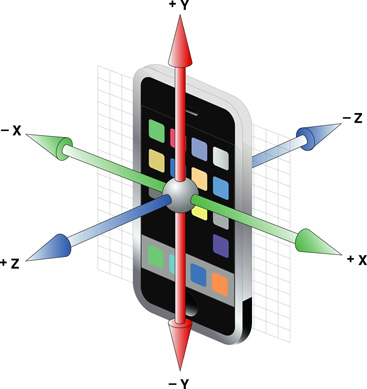
\includegraphics[width=8cm]{../img/accelerometer-axis.jpg} }}%
		\caption{The X, Y and Z axis af a smart phone device}%
		\label{fig:XYZ-Axis}% 
	\end{figure}
	
	This measurement shows that falling, is indicated by a significant drop in acceleration towards the earth's gravitational pull, signaling that the device is moving towards a free fall state, see figure \ref{fig:Pattern-Falling}. This drop is then followed by an acceleration spike as the device hits the ground. If a person were to get seriously injured due to a fall s/he would usually remain still on the ground for a period of time. Acceleration would thus gradually go back to the normal \textit{1g} indicated by the flat line after the peak. 
	
	\begin{figure}[H]
		\centering
		\subfloat{{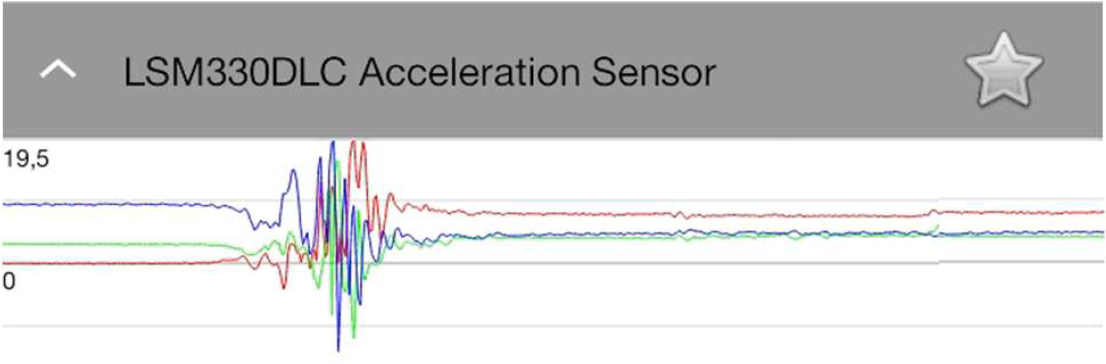
\includegraphics[width=8cm]{../img/Falling.png} }}%
		\caption{The typical pattern of falling}%
		\label{fig:Pattern-Falling}%
	\end{figure}
	
	
	Walking shows a completely different pattern. As can be seen in figure \ref{fig:Pattern-Walking}, the changes in acceleration are not rapid like in the previous example. They are also repetitive, meaning that there is no longer period of non-movements after any of the peaks. The peaks themselves are also less significant than in the case of falling shown above. This implies that walking is easily distinguished from falling.
	
	\begin{figure}[H]
		\centering
		\subfloat{{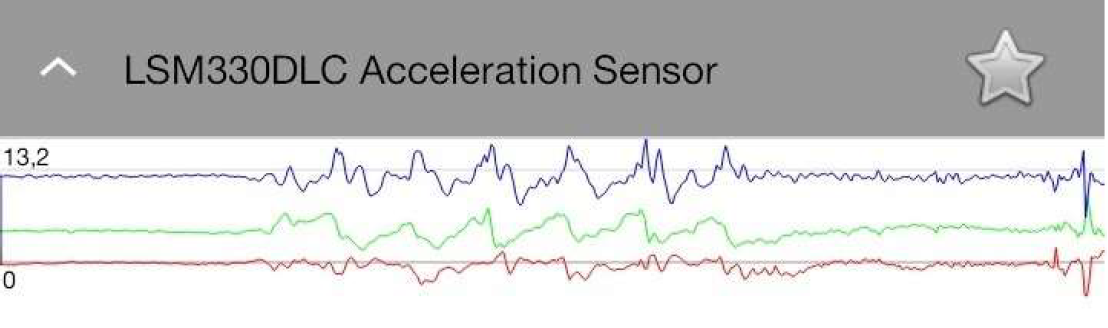
\includegraphics[width=8cm]{../img/Walking.png} }}%
		\caption{The typical pattern of walking}%
		\label{fig:Pattern-Walking}%
	\end{figure}
	
	
	 Sitting down on a surface shows a similar pattern to falling with regards to a sudden drop in acceleration followed by a rapid spike and a longer period of non-movement, see figure \ref{fig:Pattern-Sittin}. The magnitude of these values are however far less than in the case of a fall and should thus be easy to single out. When a person sits down, s/he usually makes a soft movement towards the surface, which is matched by the lesser accelerational magnitude in all three directions \textit{X, Y} and \textit{Z}.
	 
	 \begin{figure}[H]
	 	\centering
	 	\subfloat{{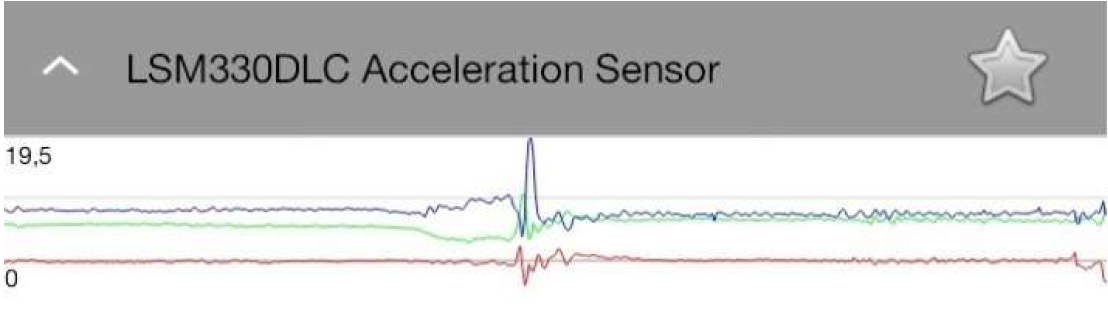
\includegraphics[width=8cm]{../img/Sitting_down.png} }}%
	 	\caption{The typical pattern of sitting down}%
	 	\label{fig:Pattern-Sittin}%
	 \end{figure}
	
	Jumping is according to Yildirim et al. the hardest pattern to distinguish from a fall, see figure \ref{fig:Pattern-Jumping}. The pattern has a sudden drop in acceleration, followed by a large spike as the jumper crouches and accelerates upwards. After this comes yet another sudden drop in acceleration as the jumper reaches the maximum altitude and starts falling back to earth again. From this part the pattern is almost identical to that of falling. When the jumper falls back to earth, the acceleration drops and then causes another huge spike as s/he hits the ground. When thinking about it, jumping and falling are in fact similar motional types, with the difference that jumping is prefixed by a drop and a spike before becoming an actual fall. The main challenge here is thus to be able to differentiate this from an unintentional falling accident.
	
	\begin{figure}[H]
		\centering
		\subfloat{{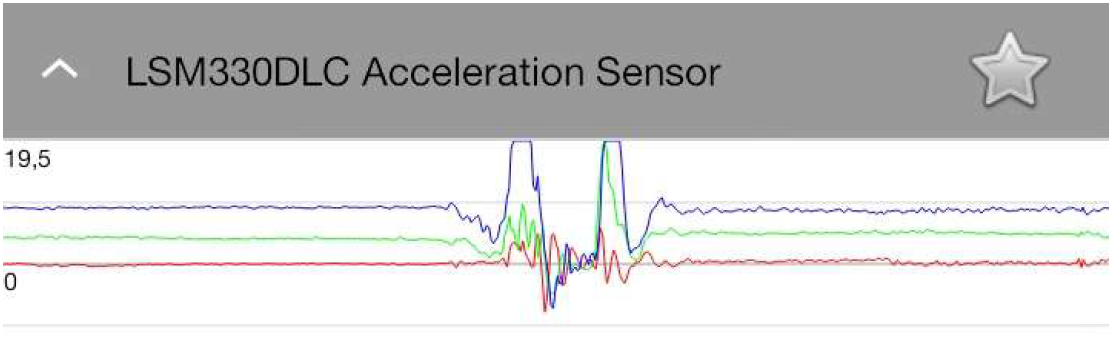
\includegraphics[width=8cm]{../img/Jumping.png} }}%
		\caption{The typical pattern of jumping}%
		\label{fig:Pattern-Jumping}%
	\end{figure}
	
	\subsection{Approach by Abbatea et al.}
	Abbatea et al. takes the above approach further by trying to establish a more sophisticated algorithm that utilizes more than merely just an acceleration vector compared to a threshold value to distinguish a fall like motional pattern from other types of ADL. Their thesis rely on several guidelines which among other include: 
	\begin{itemize} 
		\item "Detection of falls should be carried out using only acceleration-based information. Previous work demonstrated that acceleration is the most reliable information that can be used in detecting a fall, while other kinematic data, such as angular velocity, is less relevant." \cite[p~3]{piza_uni}
		
		\item "Still for usability reasons, the fall detection algorithm should work only with the magnitude of acceleration and not with the values along each of the three accelerometer’s axes, as this, again, would require a known and fixed orientation of the device with respect to the user’s body." \cite[p~3]{piza_uni}
	\end{itemize}
	
	The latter identifies the importance of calculating the resultant vector that comprises the sum of all three vectors \textit{X}, \textit{Y} and \textit{Z}. Vector length can be calculated in accordance to equation \ref{vectorlength}.
	
	\begin{equation}
	\label{vectorlength}
	|\vec{v}|=\sqrt{x^2+y^2+z^2}
	\end{equation}
	
	This vector is the overall acceleration imposed on the device (and possibly the person carrying it). They proceed by defining a \textit{fall-like-event} as "an acceleration greater than \textit{3g} followed by a period of \textit{2500ms} without further peaks exceeding the threshold." \cite[p~5]{piza_uni}. They further argue that the threshold \textit{3g} is chosen since it has been widely used in other types of fall detection systems. According to their experiments, a post-fall event usually means that the body of the unfortunate becomes lying still on the ground after a period of about \textit{1000ms}. This interval, which resides within the \textit{2500ms} interval prior to fall detection, is often due to minor peaks following the main impact as a result of that parts of the body/device may hit the ground at different times. 
	
	Abbatea et al. tries to establish their algorithm using a \textit{finite-state-machine} with five distinct states, seen in figure \ref{fig:abbatea-state-machine}.
	
	\begin{itemize}
		\item The \textit{sampling} state is the normal state that the process resides in until \textit{threshold-peak} is detected.
		
		\item When a peak occurs that exceeds the threshold value of \textit{3g} the state is transferred to \textit{post peak}. Well in this state, a bouncing timer of \textit{1000 ms} is started. If another peak exceeding the threshold occurs during this time, bouncing timer is reset, otherwise the state machine moves on to the \textit{post fall} state when the timer fires.
		
		\item In the \textit{post fall state} no peaks exceeding the threshold are allowed during \textit{1500 ms}, or the system goes back to the \textit{post peak} state. The purpose if this state is to check for activity (movement). If another peak occurs, it signals that either is the presumed fall not finished, or the subject is moving and this should not regarded as a fall. 
		
		\item When the \textit{post fall timer} fires after 1500 ms, the state machine moves on to the \textit{activity test} state. In this test, if movement exceeding certain thresholds are detected, it once again signals that activity is found and that this was indeed not an actual fall but rather a result of ADL. 
		
	\end{itemize}  
	
	
	\begin{figure}[H]
		\centering
		\subfloat{{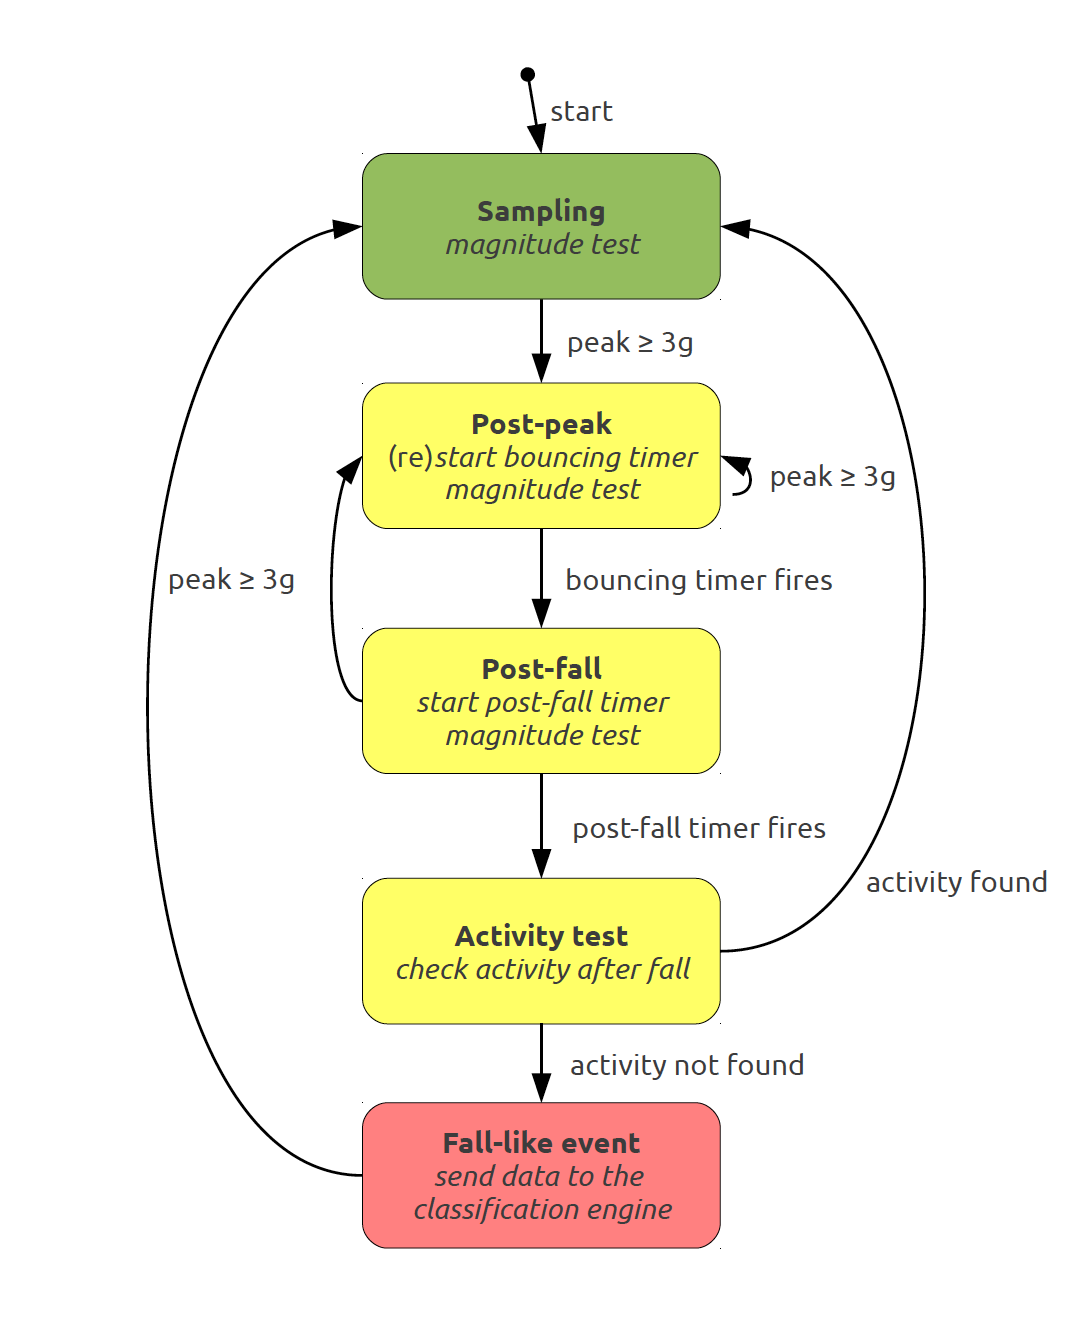
\includegraphics[width=8cm]{../img/Abbatea_finite_state_machine.png}}}%
		\caption{The sensing process discussed in Abbatea et al.}%
		\label{fig:abbatea-state-machine}%
	\end{figure}
	
	
	
	If a fall like event has passed through the  \textit{activity test} (the last state in the state machine), it is fed through a feature extractor, which analyses the data and extracts specific and predefined features of the data set. The features represent certain particular types of data that can be found by analysing the wave form collected when sampling the accelerometer. Before describing the features they defined 3 properties:
	\begin{itemize}
		\item \textit{Peak time} - The time of the detected peak (which is followed by \textit{2500 ms} without further peaks).
		\item \textit{Impact end} - The time of the last impact exceeding \textit{1,5 g} after \textit{peak time + 1000 ms}
		\item  \textit{Impact start} - The time of the last sample below \textit{0,8 g} before \textit{peak time} or \textit{peak time} if not found. 
	\end{itemize}
	They used a total of 8 features:
	
	\begin{itemize}
		\item \textit{Average absolute Acceleration Magnitude Variation} - The average magnitude of the acceleration samples, collected in the time window (\textit{win}) of \textit{1000 ms} centred at the middle between \textit{impact start} and \textit{impact end}, can be calculated according to the formula in \ref{fig:aamv-formula}. 
		
		
		\begin{figure}[H]
			\centering
			\subfloat{{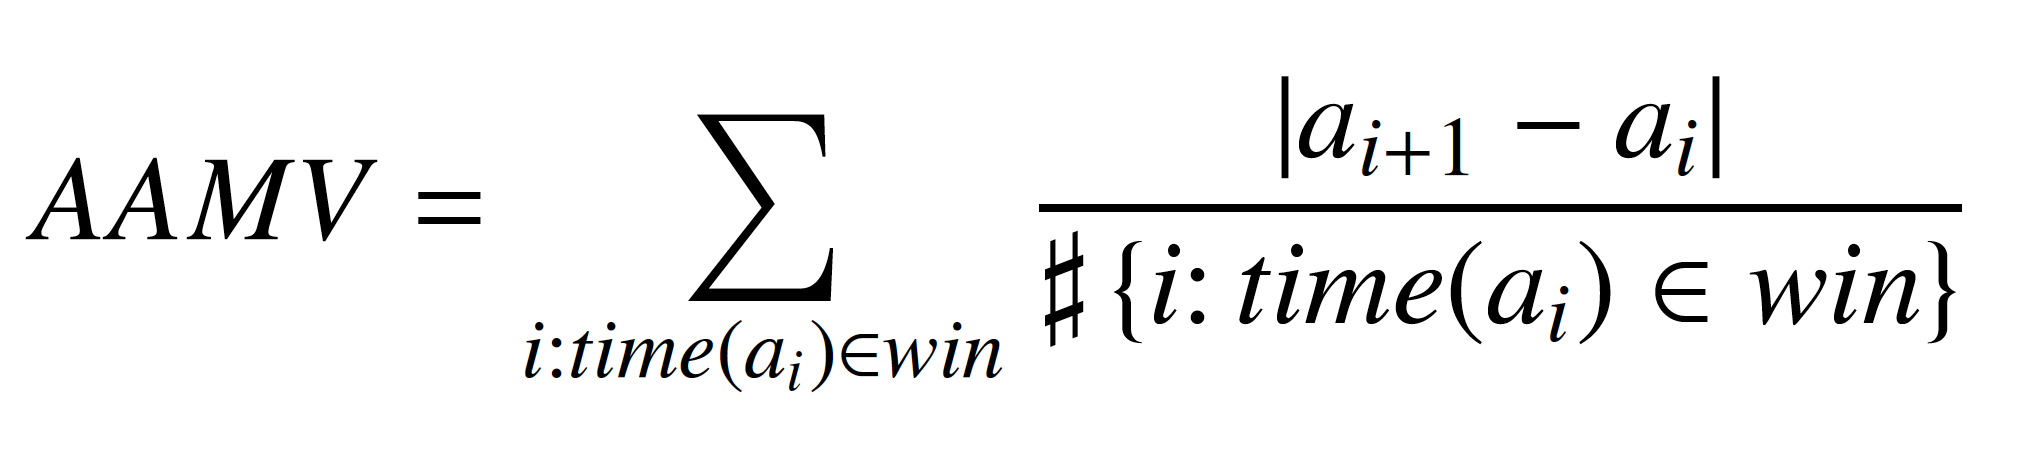
\includegraphics[width=8cm]{../img/AAMV_formula.png}}}%
			\caption{The formula for calculating AAMV \cite{piza_uni}}%
			\label{fig:aamv-formula}%
		\end{figure}
		
		\item \textit{Impact Duration Index} - The duration of the impact peak, exceeding the threshold.
		\item \textit{Maximum Peak Index} - The highest value of the peak found in the interval [\textit{impact start}, \textit{impact end}]
		
		\item \textit{Minimum Valley Index} - The lowest value of acceleration magnitude found in the interval [\textit{impact start} - 500 ms, \textit{impact end}]
		
		\item \textit{Peak duration index} - The duration represented by \textit{impact end - impact start}
		\item \textit{Activity Ratio Index} - The number of samples in a \textit{700 ms} time window centred between \textit{impact start} and \textit{impact end} that are not in [\textit{0.85g, 1.3g}] divided by the number of total number of samples in that time window.
		
		\item{Free Fall Index} - The average acceleration magnitude found in an interval up to \textit{200 ms} before \textit{peak time} till up to \textit{400 ms} before peak time.
		
		\item{Step count index} - The amount of valleys and peaks in the interval [\textit{peak time - 2200 ms}, \textit{peak time}]
	\end{itemize}
	
	These extracted features are then fed in to a neural network with eight inputs and four neurons in a single hidden layer (\textit{neural network are thoroughly described in this free on-line book}  \cite{neural_networks}). The output layer consists of the four classes (\textit{Falls, Sitting/Lying, Jump/Run/Walk, Hitting sensor}). The network outpost the estimated probability of the event on all four classes and if the probability for the \textit{Falls}  class exceeds all other probabilities, the event is classified as a fall.
	
	
	\newpage
	\section{Methods and Methodology}
	
	This chapter describes the research strategy and the methodologies used in the study, and how each methodology contributes to answering the research questions.
	
	\subsection{Research Strategy}
	
	This section describes research methods in general, and how the methods are adopted in this thesis.
	
	\subsubsection{Quantitative and qualitative methods}
	
	Research methods are often divided in two classes, \textit{quantitative} and \textit{qualitative} methods.
	
	\textit{Quantitative} methods are distinguished by the use of measurable data \cite[p~54]{borrego}. This data can be numbers such as a measured distance, collected statistics, the outcome of an experiment, etc. Quantitative methods are a way for the researcher to take an objective approach.
	
	\textit{Qualitative} methods on the other hand, is characterized by the collection of textual data \cite[p~55]{borrego}. This data can be interviews, surveys, observations, etc. Qualitative methods emphasis the importance of context in which the study is performed.
	
	\subsubsection{Inductive and deductive methods}
	
	An \textit{inductive} research method can be viewed as a bottom-up approach, where the researcher begins by collecting data that is relevant to the subject. After that, the data is analyzed, with the intention to develop a theory that explains the patterns observed in the data.
	
	A \textit{deductive} method is a top-down approach, where a hypothesis is developed from existing theory. After the hypothesis is formulated, it is tested with the intent to confirm or falsify it.
	
	\subsubsection{Case studies}
	
	Case studies makes it possible for a researcher to closely examine a specific phenomenon. They can be explorative, explanatory or descriptive \cite[p~4]{yin}. A case study is often limited to a small number of people or a small geographic area to perform an in-depth examination, and can be a good research method for answering questions starting with "how" or "why".
	
	\subsubsection{Adopted Methods}
	
	For our research, a qualitative approach seems to be the most appropriate. It will be a case study that explores the possibility of creating a fall detection application, answering how this should be done. The research will be deductive, starting with the hypothesis that this kind of application can be created, trying to confirm the hypothesis. 
	
	In order to give an answer to the first question of our problem statement, RQ1, we need to solve a number of sub problems. The first problem is to find a suitable algorithm that can achieve accurate fall detection, since without a good algorithm it will be impossible to make a useful implementation. The second problem is to implement this algorithm in a mobile application using the sensors available in smart phones. This could be troublesome if the algorithm expects better sensors than what is available in the smart phone. The third sub problem is to evaluate the implementation. We will evaluate the accuracy of the fall detection, that is how many of the detected falls are actual falls, and how many actual falls are not detected. Another part of the evaluation will be to evaluate the application's impact on battery life. For these sub problems we formulate specific questions that we will need to answer in order to answer the problem statement.
	
	\begin{itemize}
		\item What algorithm should be used to accurately detect a fall?
		\item How can technology available in smart phones be used to implement an algorithm for fall detection?
		\item How can accuracy and performance be improved when implementing fall detection in a smart phone?
	\end{itemize}
	
	\parag{Literature Study}
	The literature study that we will perform will focus on finding an algorithm that can be used to accurately detect a fall. Performing a literature study will give us a wider understanding of the subject as well as a good starting point for the study. The result of the literature study will show which algorithm for fall detection that would be proposed by previous studies. We will use this algorithm as a starting point for our own implementation, where we will try to improve the algorithm. The outcome of the literature study is presented in the theoretical background.
	
	\parag{Case Study: Developing a mobile application}
	The second part of our research will be a case study where we implement a fall detection system. We will use the algorithm found in the literature study and implement it for Android and iOS using the sensors available in the smart phones. Developing the application will give us an opportunity to test the algorithm on real devices, and a platform where we can experiment in order to improve the algorithm. The result of the development will give us the ability to answer how technology available in smart phones can be used to implement the algorithm found in the literature study.
	
	\parag{Evaluating the implemented mobile application}
	The third part of our research will be to evaluate the implemented algorithm by performing experiments where the mobile application is used to detect falls. This evaluation will focus on how accurate the application is, but also on how it affects the battery life of the device.
	
	\subsubsection{Research Process}
	
	In this thesis project, the work is divided in phases as seen in figure \ref{fig:research-process}. The first phase, the problem statement serves to formulate the problem that the thesis will try to solve. The second phase is the literature study, where reports from earlier studies are collected and read to give us a deeper understanding of the subject. The third phase is the analysis phase, where the results of the literature study is analysed in order to find an algorithm that will be suitable as a starting point for the application. After the analysis phase the case study begins, where we implement the mobile application. After the case study phase the evaluation phase starts, where the final version of the application developed in the case study is evaluated. After that, the conclusion phase starts, where the results are summarized and conclusions formulated. 
	
	\begin{figure}[H]
		\centering
		\subfloat{{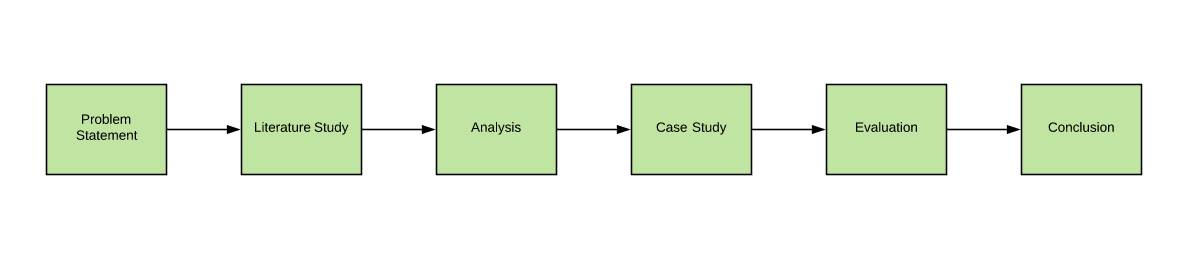
\includegraphics[width=14cm]{../img/method-phases.png} }}%
		\caption{The different phases in the thesis project}%
		\label{fig:research-process}%
	\end{figure}
	
	\subsection{Design and Implementation of Application}
	
	To develop the mobile application we will use an iterative development method. By using an iterative method we will make sure that the most important features are developed first, since we will develop the most important features in the first iteration and only after that continue with the less important features. This will help us  minimize the risks in the project. If the project would suffer from lack of time, we would at least have developed the most important features already. The project method that we will be using will be similar to Scrum, although since we are only two developers, the team involved in development will be much smaller than the typical agile team.
	
	We will divide the work in such a way that one of us will develop the Android implementation, and the other will develop the iOS implementation. By dividing the work in this fashion we can implement similar features in both applications without the risk of writing conflicting code. Another reason for dividing the work is that it will help us to have equal focus on both the Android and iOS implementation.
	
	\subsubsection{Development Process}
	
	The development process will follow the outline in figure \ref{fig:development}. The process will start with design, where an initial version of the application is designed, with only a limited set of features. We will then implement those features, and then evaluate the developed features and the application. After that we will go back to development, and based on the outcome of the development we will either start over, or continue with new features.
	
	\begin{figure}[H]
		\centering
		\subfloat{{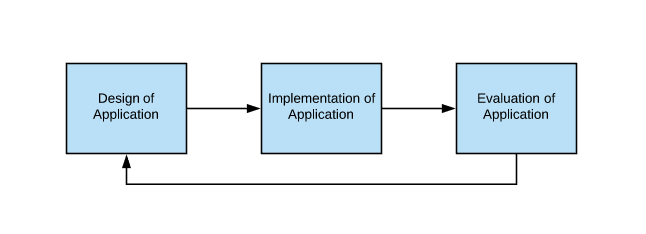
\includegraphics[width=14cm]{../img/method-development.png} }}%
		\caption{The application development process}%
		\label{fig:development}%
	\end{figure}
	
	\subsubsection{Development Environment}
	
	The application will be divided in two implementations, one for Android and one for iOS. The development environment will be slightly different for Android and iOS. 
	
	\parag{Android}
	The Android application will be developed using Android Studio, since it is the official development environment.
	
	\parag{iOS}
	The iOS application will be partly developed in Xcode, since it is the official IDE, and partly in Jetbrains AppCode since it is superior to Xcode when it comes to re-factoring code, code completion, etc. Xcode will be used for building graphical interfaces, but the coding will be done in AppCode.
	
	\subsection{Evaluation Methods}
	
	This section describes how the developed application will be evaluated. Evaluating the application is important since it will show how well it solves the problem.
	
	\subsubsection{Evaluating accuracy}
	
	The first step in the evaluation of the application will be to perform crash tests where we measure how well the application detects a fall, by dropping a mobile phone running the application several times from a height that we define as a fall and count the number of reported falls. The same test can then be performed with an existing application to compare how well the implemented algorithm compares to existing technology.
	
	Another measurement will be to drop the mobile phone running the application from a height that we do not define as a fall, and count how many falls are falsely detected. This number will also be compared with the result of running the same test with an existing application.
	
	Yet another test will be to perform daily activities that can trigger a fall detection system, even though it is not a fall. Theses activities can be running, or walking with the phone in the pocket. A good fall detection software will not report many of these as falls. This will also be compared against an existing application.
	
	\subsubsection{Evaluating battery life}
	
	To evaluate how the application affects the battery life of the mobile phone, we will use the native functionality in the operating system available on Android and iOS respectively to measure the specific applications power consumption.
	In combination with this, we will also perform tests where we run the application for a certain amount of time and note how much battery life is left and compare this value with the percentage left after not running the application for the same amount of time.
	
	\newpage
	\section{Challenges and Possibilites}
	
	This chapter describes the different challenges that were encountered during the research project, how they were solved and why they were solved this way.
	
	\subsection{Changes in the state machine}
	
	The work made by Abbatea et al. served as a good starting point for our research project, since their work is very similar to what we want to achieve. When reading their report we thought that their work could be improved on some points. One of them were the state machine. The state machine used by Abbatea et al., presented in figure \ref{fig:abbatea-state-machine}, were lacking a state for free falling, that is, when the acceleration magnitude drops below \textit{g}. Their report describes that their state machine had some trouble distinguishing from a real fall and simply hitting the sensor. These cases were later filtered out by their machine learning module, which were examining if the acceleration magnitude had dropped below \textit{g} or not. For this reason we though that it would be an improvement to detect the free falling in the state machine and filter out the cases that had no free fall before the impact. We did this by introducing a state called \textit{Falling} in which the acceleration magnitude must be lower than a certain threshold.
	
	\subsection{Using a neural network}
	
	Initially we had not intended to implement a machine learning model in the project, since we did not think that it would be much better than just using a state machine. But since Abbatea et al. had used a neural network for their implementation we decided to give it a try. We defined the features that were fed into the neural network slightly different. The first main difference where that we did not include their \textit{Activity Ration Index} since the difference in value for that feature between the different classes were small. The other main difference were that we did not use their \textit{Step Count Index}, since we defined \textit{Number of peaks prior to impact} and \textit{Number of valleys prior to impact} instead, distinguishing from peaks and valleys instead of just counting steps. 
	
	After we had decided which features to extract we started to experiment with the neural network. We started out with the same neural network that they had used, with 8 inputs, 8 neurons and 4 output classes, but we fed the network with our 8 features instead of theirs. While experimenting with collecting data and training the model we realized that one of the 4 output classes, \textit{Hit device}, were never encountered. This is probably due to the difference in the state machine, indicating that our state machine had successfully filtered out that class before reaching the machine learning model. Since that class were never detected there were no need to keep it in the neural network, so we removed it.
	
	To see if the accuracy in the model could be improved while training, we experimented with adding additional layers of neurons. We tried to use 2, 3 or 4 layers of neurons instead of just one, but the experiments showed that the accuracy in the model decreased, for this reason we removed the additional layers and went back to a single layer of neurons.
	
	
	
	
	
	
	\subsection{Running the application in background}
	
	When implementing fall detection in a smart phone it is important that the application can run in background mode. By background mode we hereby refer to when the app is not present on the screen. This means that the app is either behind another application when the user is using the device, or when the device itself is locked. Since the application is supposed to run for a long time we cannot expect the user to have the application visible in foreground all the time. This turned out to be quite troublesome, at least in iOS, this section describes how this challenge were solved on the different platforms.
	
	\subsubsection{Android}
	
	In Android, it is possible to define a background task by creating a class that extends \texttt{android.app.Service}. We chose to create a Service that communicates with our state machine and classification engine, and if a fall is  detected the Service broadcasts the fall to any registered \\ \texttt{android.content.BroadcastReceiver}.
	
	\subsubsection{iOS}
	iOS is very strict with regards to allowing applications to do background processing , only a few types of background tasks are allowed such as playing audio, getting location updates or downloading content from the internet to mention some. However, by signing up for one of the allowed background modes, the app can be kept alive in the background and thus perform other tasks in the meantime such as sampling the accelerometer. Since location updates is needed to alert emergency contact about the users location in case of a fall accident, our choice of background mode is location services.
	
	\newpage
	\section{Fall Detection Application: Design and Implementation}
	
	
	\subsection{Architecture outline}
	The overall architecture of the application consists of several steps. All readings from the accelerometer is continuously pushed to a ring buffer. 	This ring buffer holds the last 8 seconds of accelerometer data. On top of this, a \textit{finite state machine} is used as a first barrier to filter out the most common movements of the device. If a fall-like event were to manipulate the state machine into its final state, the ring buffer is transferred over to a \textit{Feature Extractor}. In this step, the buffer is analyzed and a total of 8 "features" are extracted (as similar to the Abbatea et el approach). These features represent important aspects of the movement of the device for the last 8 seconds. 
	
	The 8 features are then put inside a data-object and fed into a \textit{Classification Engine} which consists of a neural network. This classification engine have the responsibility to classify the event based on the given features. The output classes of the neural network are; \textit{Fall}, \textit{Jump} and \textit{Run/Walk}. The neural network calculates the independent probability of the event's belonging to each of the three classes. If the probability of the event belonging to the \textit{Fall} class exceeds the other two, the event is considered a fall. 
	
	In the case of an event being classified as a fall, the application will present a screen along with a sonic alarm signal. The user will then have 45 seconds to discard the event or a message will be sent to a set of predefined contacts, notifying them about what´s happened.
	
	\begin{figure}[H]
		\centering
		\subfloat{{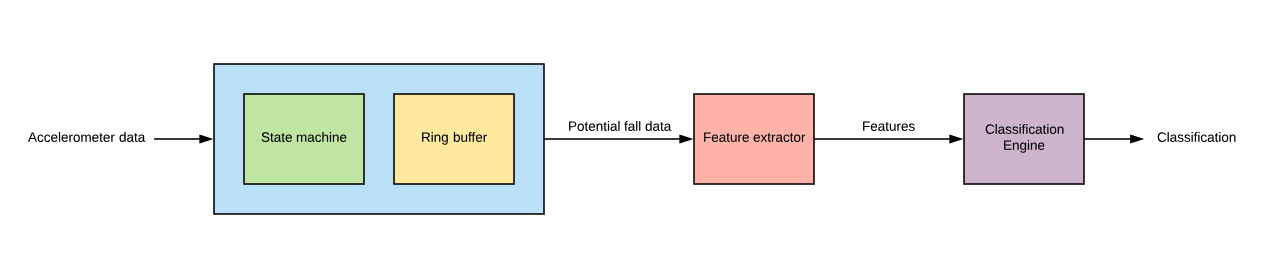
\includegraphics[width=14cm]{../img/arch-outline.png} }}%
		\caption{Outline of the fall detection application}%
		\label{fig:arch-outline}% 
	\end{figure}
	
	\subsection{Using the accelerometer}
	Using the accelerometer on the Android and iOS system is similar. Updates from the accelerometer are pushed to listening code that acts upon those updates. Updates come in the form of an data-object containing information about the device's acceleration on all three axes (\textit{X}, \textit{Y} and \textit{Z}) at that moment in time. The accelerometer's update frequency is configurable on both Android and iOS devices and we chose an update frequency of \textit{50 Hz} since it provides a reasonable balance between accuracy in measurements and battery consumption. On each update, the resultant vector is calculated according to the formula in \ref{vectorlength} and the result is put in to the ring buffer. Given this configuration, the ring buffer have a fixed length of \(50 Hz * 8s = 400\) samples. On each new update, the resultant vector is also given to the finite state machine who will act according to the description in the next section.
	
	
	
	\subsection{Design of state machine}
	
	For basic fall detection, a finite-state machine were used, see figure \ref{fig:state-machine}. The resultant vector coming from the accelerometer is fed as input to the state machine. The state machine reads the input and changes state based on different parameters for each state. If the state machine would reach it's final state, this would mean that a potential fall has been detected. The thresholds used for the accelerometer vector is defined as Impact Threshold (IT), Upper Motionless Threshold (UMT), Lower Motionless Threshold (LMT). The upper motionless threshold is 1.5 g, the lower motionless threshold is 0.5g, and the impact thresholds are different for Android and iOS. The impact threshold is 2.5g for Android and 4g for iOS. 
	
	\begin{figure}[H]
		\centering
		\subfloat{{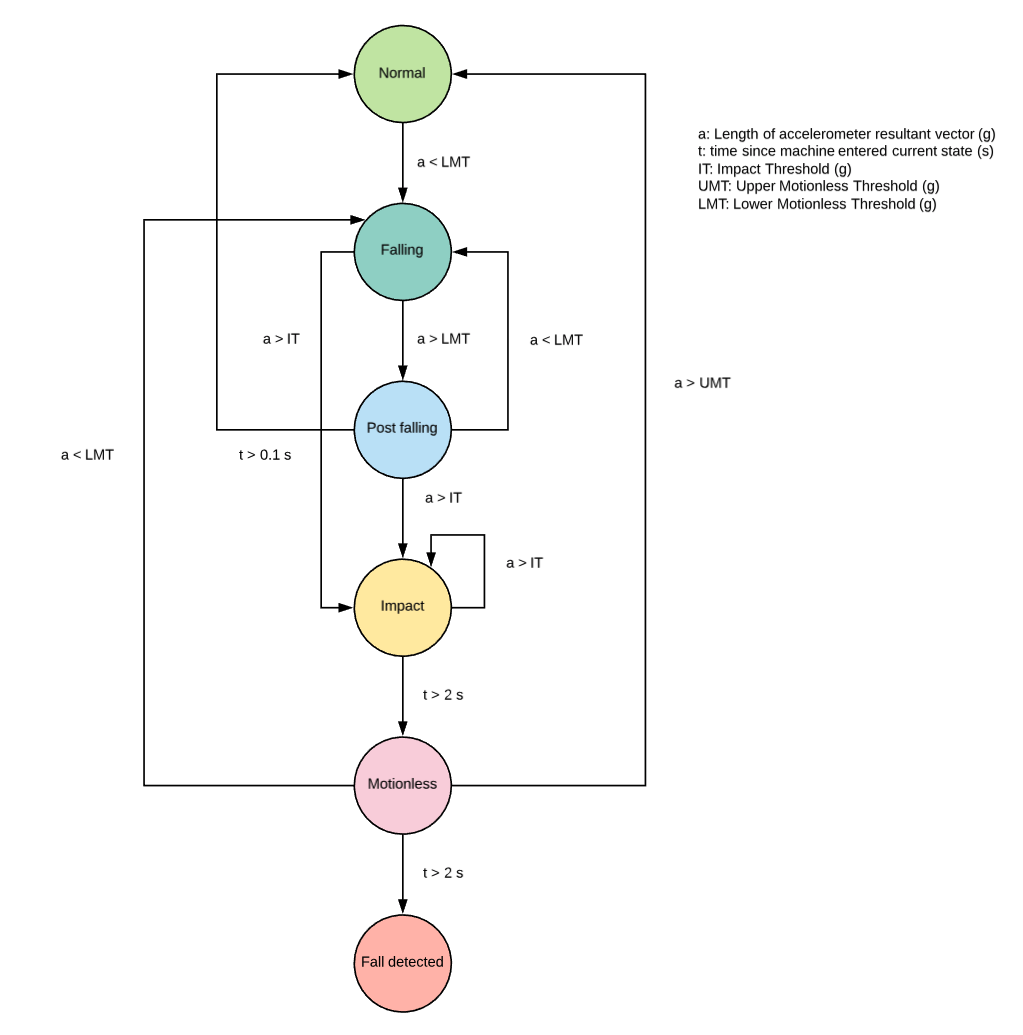
\includegraphics[width=16cm]{../img/state-machine-2.png} }}%
		\caption{Fall detection state machine}%
		\label{fig:state-machine}%
	\end{figure}
	
	\begin{figure}[H]
		\centering
		\subfloat{{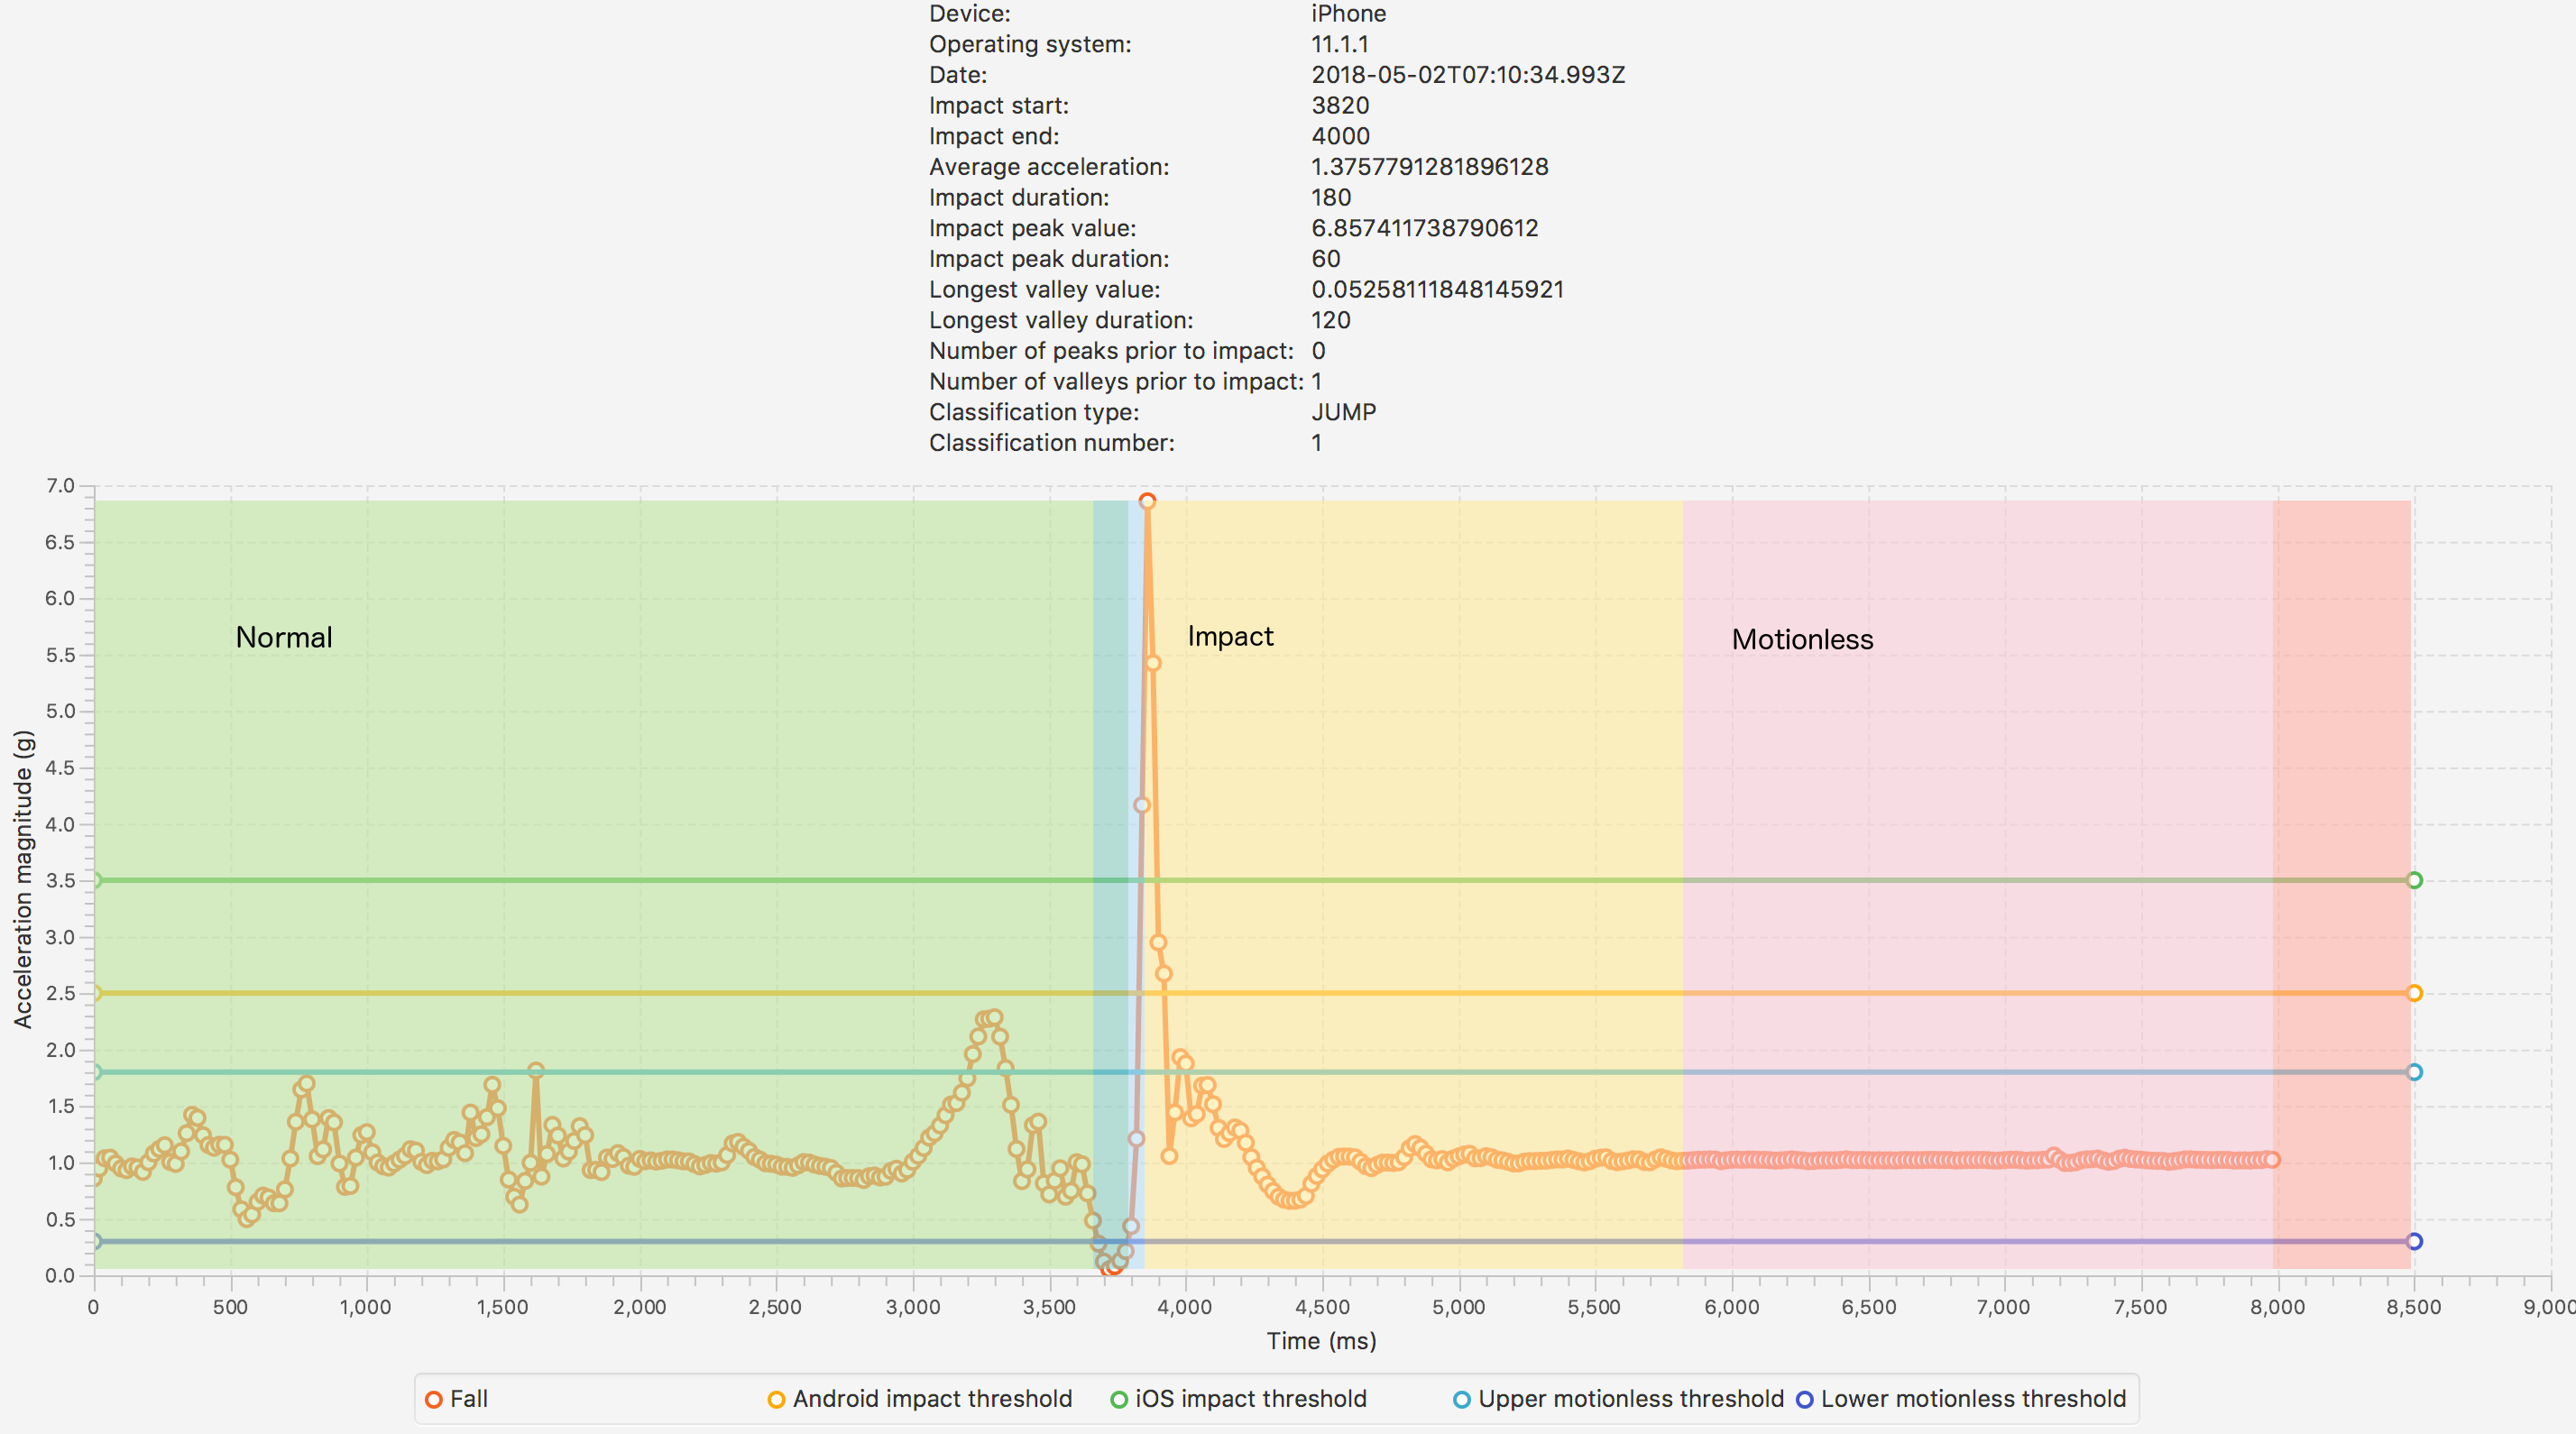
\includegraphics[width=14cm]{../img/fall-data-state-machine.png} }}%
		\caption{Visualization of how the state machine passes through the different states during a potential fall, along with the acceleration magnitude. The colors of the different states correspond to the colors of the states in figure \ref{fig:state-machine}.}%
		\label{fig:fall-data-state-machine}%
	\end{figure}
	
	\subsubsection{Normal state}
	
	The initial state, when the state machine starts is the normal state. If the length of the accelerometer resultant vector (a) exceeds the lower motionless threshold, a transition is made to the falling state.
	
	\subsubsection{Falling state}
	
	The falling state represents that the phone is falling freely, and it should have an acceleration close to zero, or at least under the lower motionless threshold. If the accelerometer vector length exceeds the lower motionless threshold but not the impact threshold, a transition is made to the post falling state. If the accelerometer vector length exceeds the impact threshold a transition is made to the impact state.
	
	\subsubsection{Post falling state}
	
	The post falling state is a state between the falling state and the impact state. It exists to allow a slight lag between the free falling and the impact. If the accelerometer vector length exceeds the impact threshold the machine enters the impact state. If the time since the machine entered the current state exceeds the time limit 0.1 s a transition is made back to the normal state. This is because no impact occurred in the allowed time window.
	
	\subsubsection{Impact state}
	
	The impact state represents that an impact has been detected. In this state anything is allowed to happen under a time limit. If the accelerometer vector length exceeds the impact threshold, a transition back to the impact state is made to reset the timer keeping track of the time since the state machine entered the current state. If the timer value exceeds the 2 s threshold a transition is made to the motionless state.
	
	\subsubsection{Motionless state}
	
	The motionless state exists to make sure that the phone is motionless after the fall. If the accelerometer vector length exceeds the upper motionless threshold, the machine goes back to the normal state. If the vector length drops below the lower motionless threshold a transition is made to the falling state.
	
	\subsubsection{Fall detected state}
	
	In the fall detected state, a potential fall has been detected. The machine takes action to inform the rest of the application that the data in the ring buffer should be analyzed to see if this was an actual fall.
	
	\subsection{Design of feature extractor}
	
	The purpose of the feature extractor is to take the data in the ring buffer and extract 8 defined features from it. The 8 features will then be used in the neural network. The features are similar to the features defined by Abbatea et al. \cite{piza_uni}, but redefined. The data coming from the ring buffer and the features defined by the feature extractor is visualized for one example case in \ref{fig:fall-data-example}.
	
	\begin{figure}[H]
		\centering
		\subfloat{{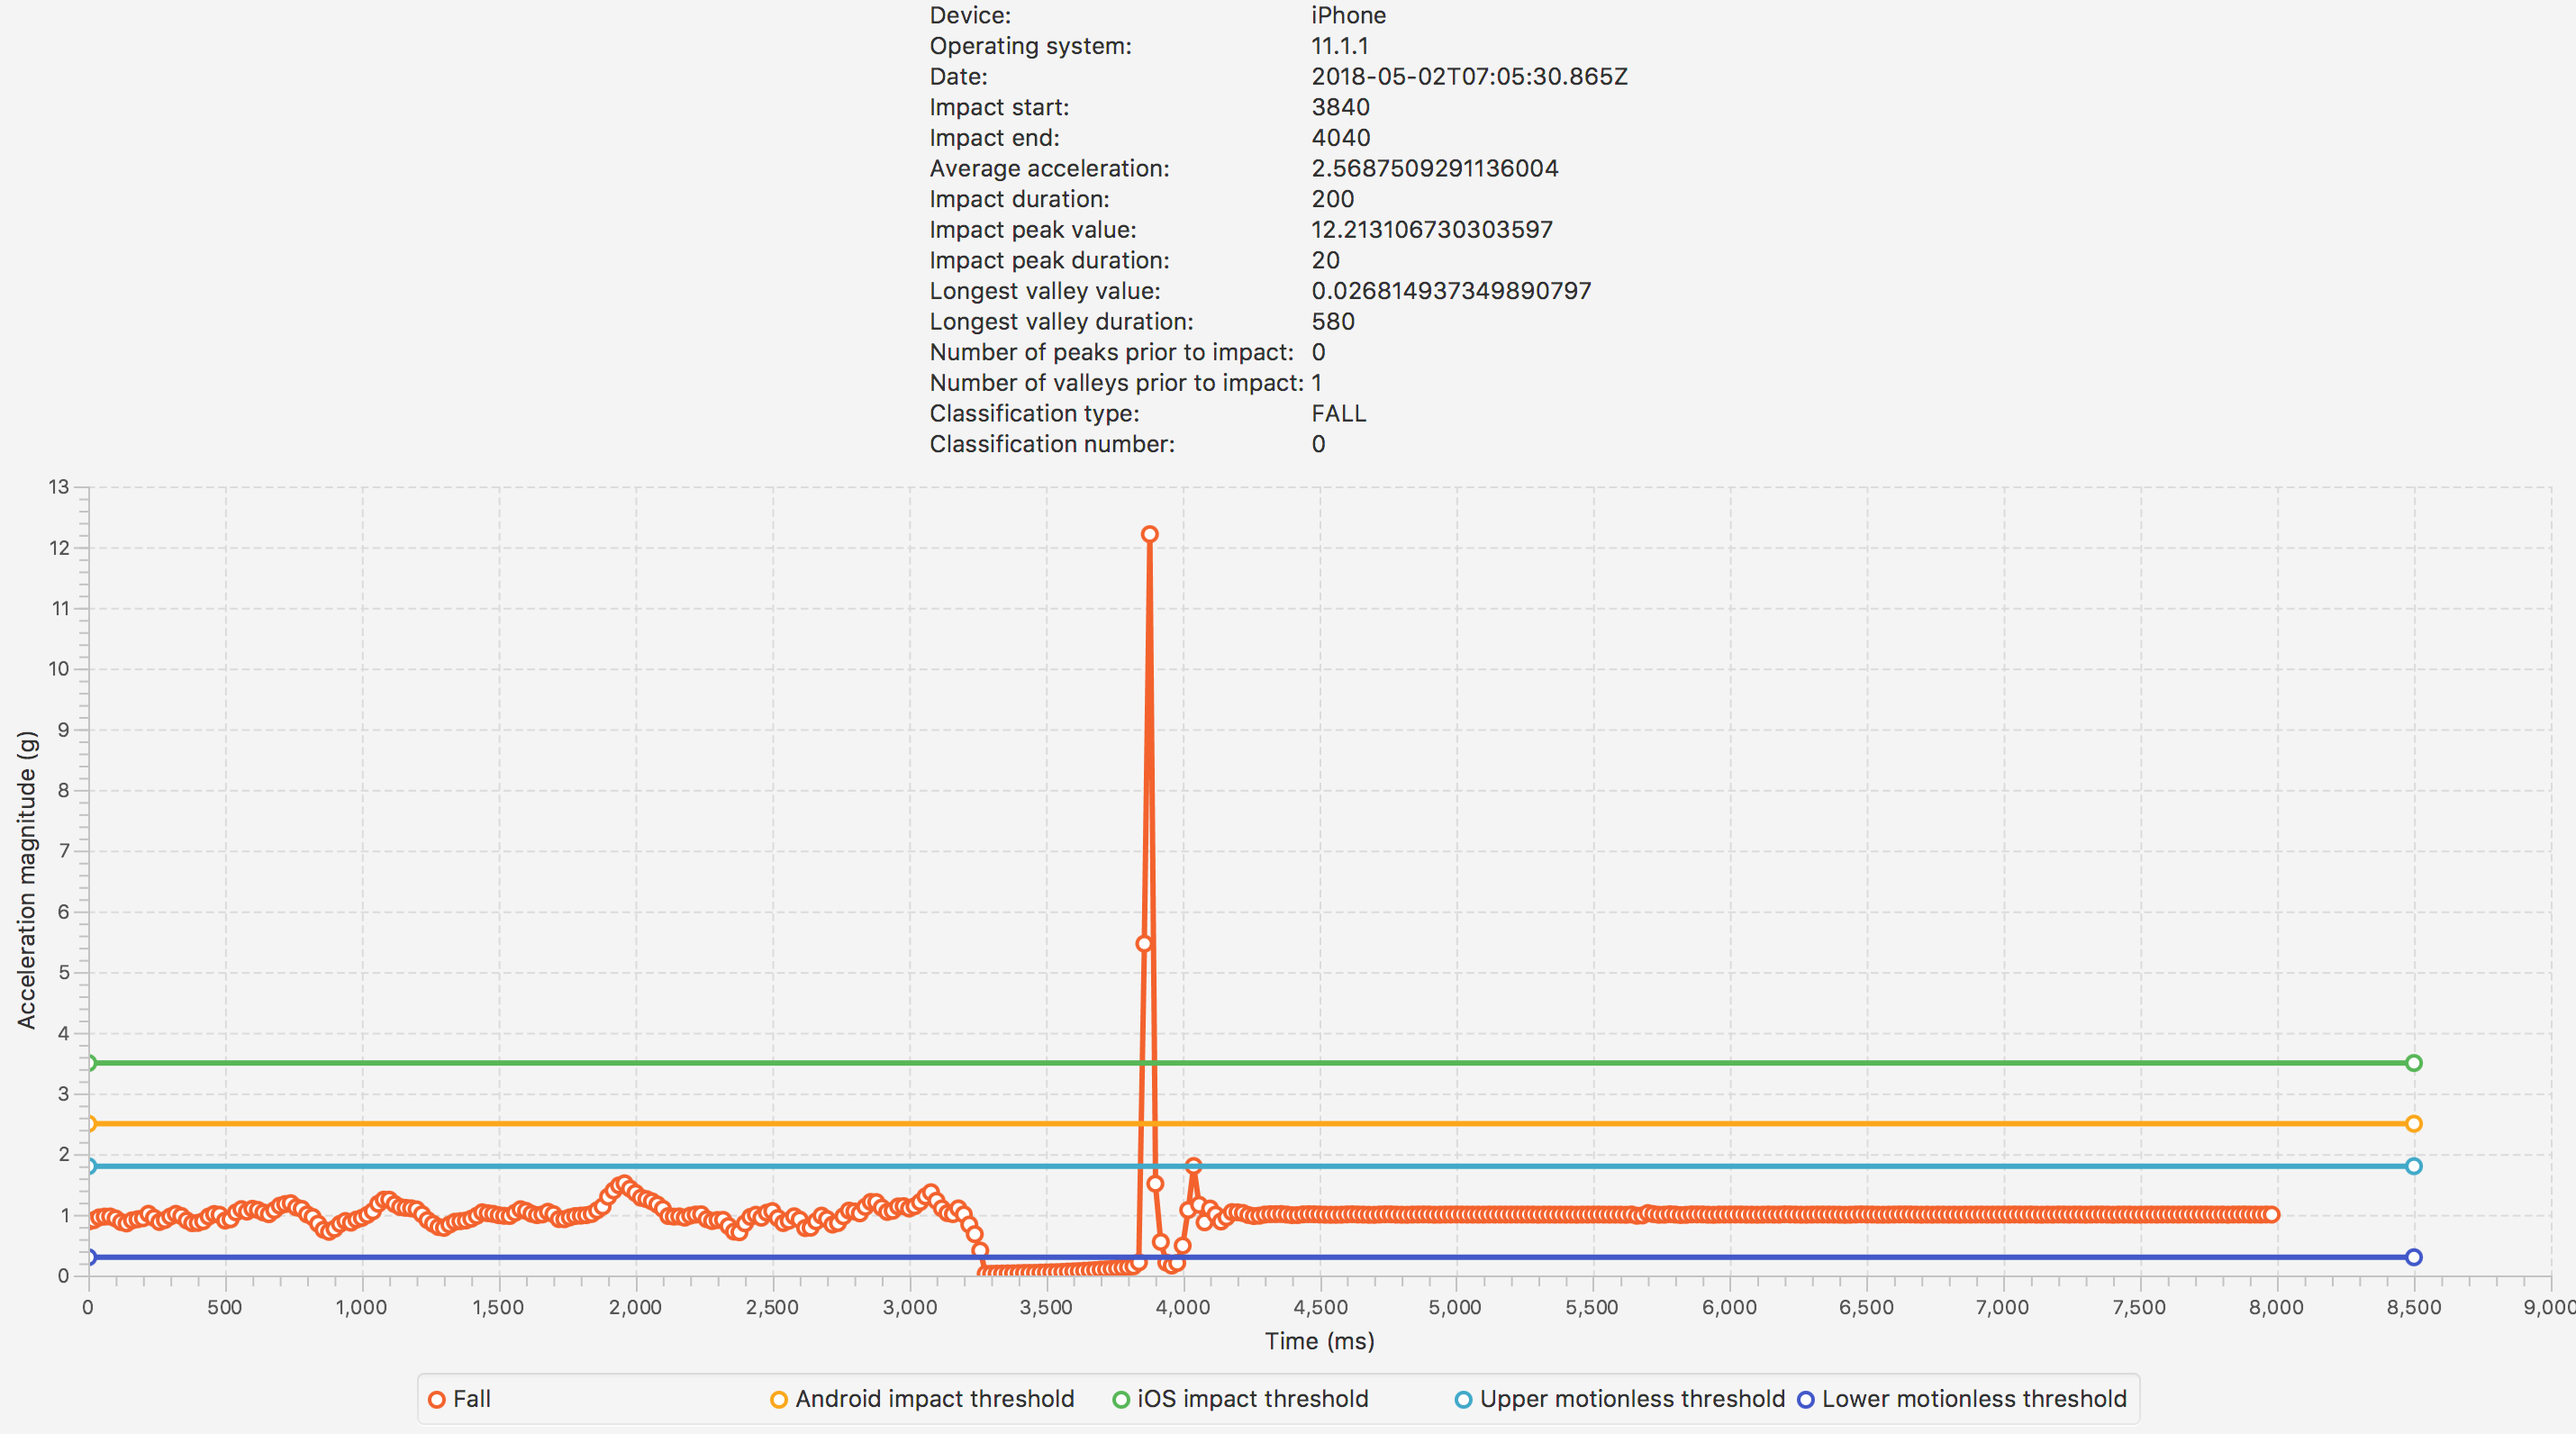
\includegraphics[width=14cm]{../img/fall-data-example.png} }}%
		\caption{Recorded data from dropping the phone. Each point on the graph represents one sample in the ring buffer. The values found by the feature extractor can be seen at the top.}%
		\label{fig:fall-data-example}%
	\end{figure}
	
	
	
	\subsubsection{Average acceleration variation}
	
	The first feature that the extractor should find is the average acceleration variation. This feature is calculated using the formula in figure \ref{fig:aamv-formula}. This feature is supposed to measure how much the acceleration variates after the initial impact peak. Figures \ref{fig:fall-data-run-ios} and \ref{fig:fall-data-run-android} shows examples of where this variation is significant, as compared to figures \ref{fig:fall-data-fall-ios} and \ref{fig:fall-data-fall-android} where the variation is small.
	
	\begin{figure}[H]
		\centering
		\subfloat{{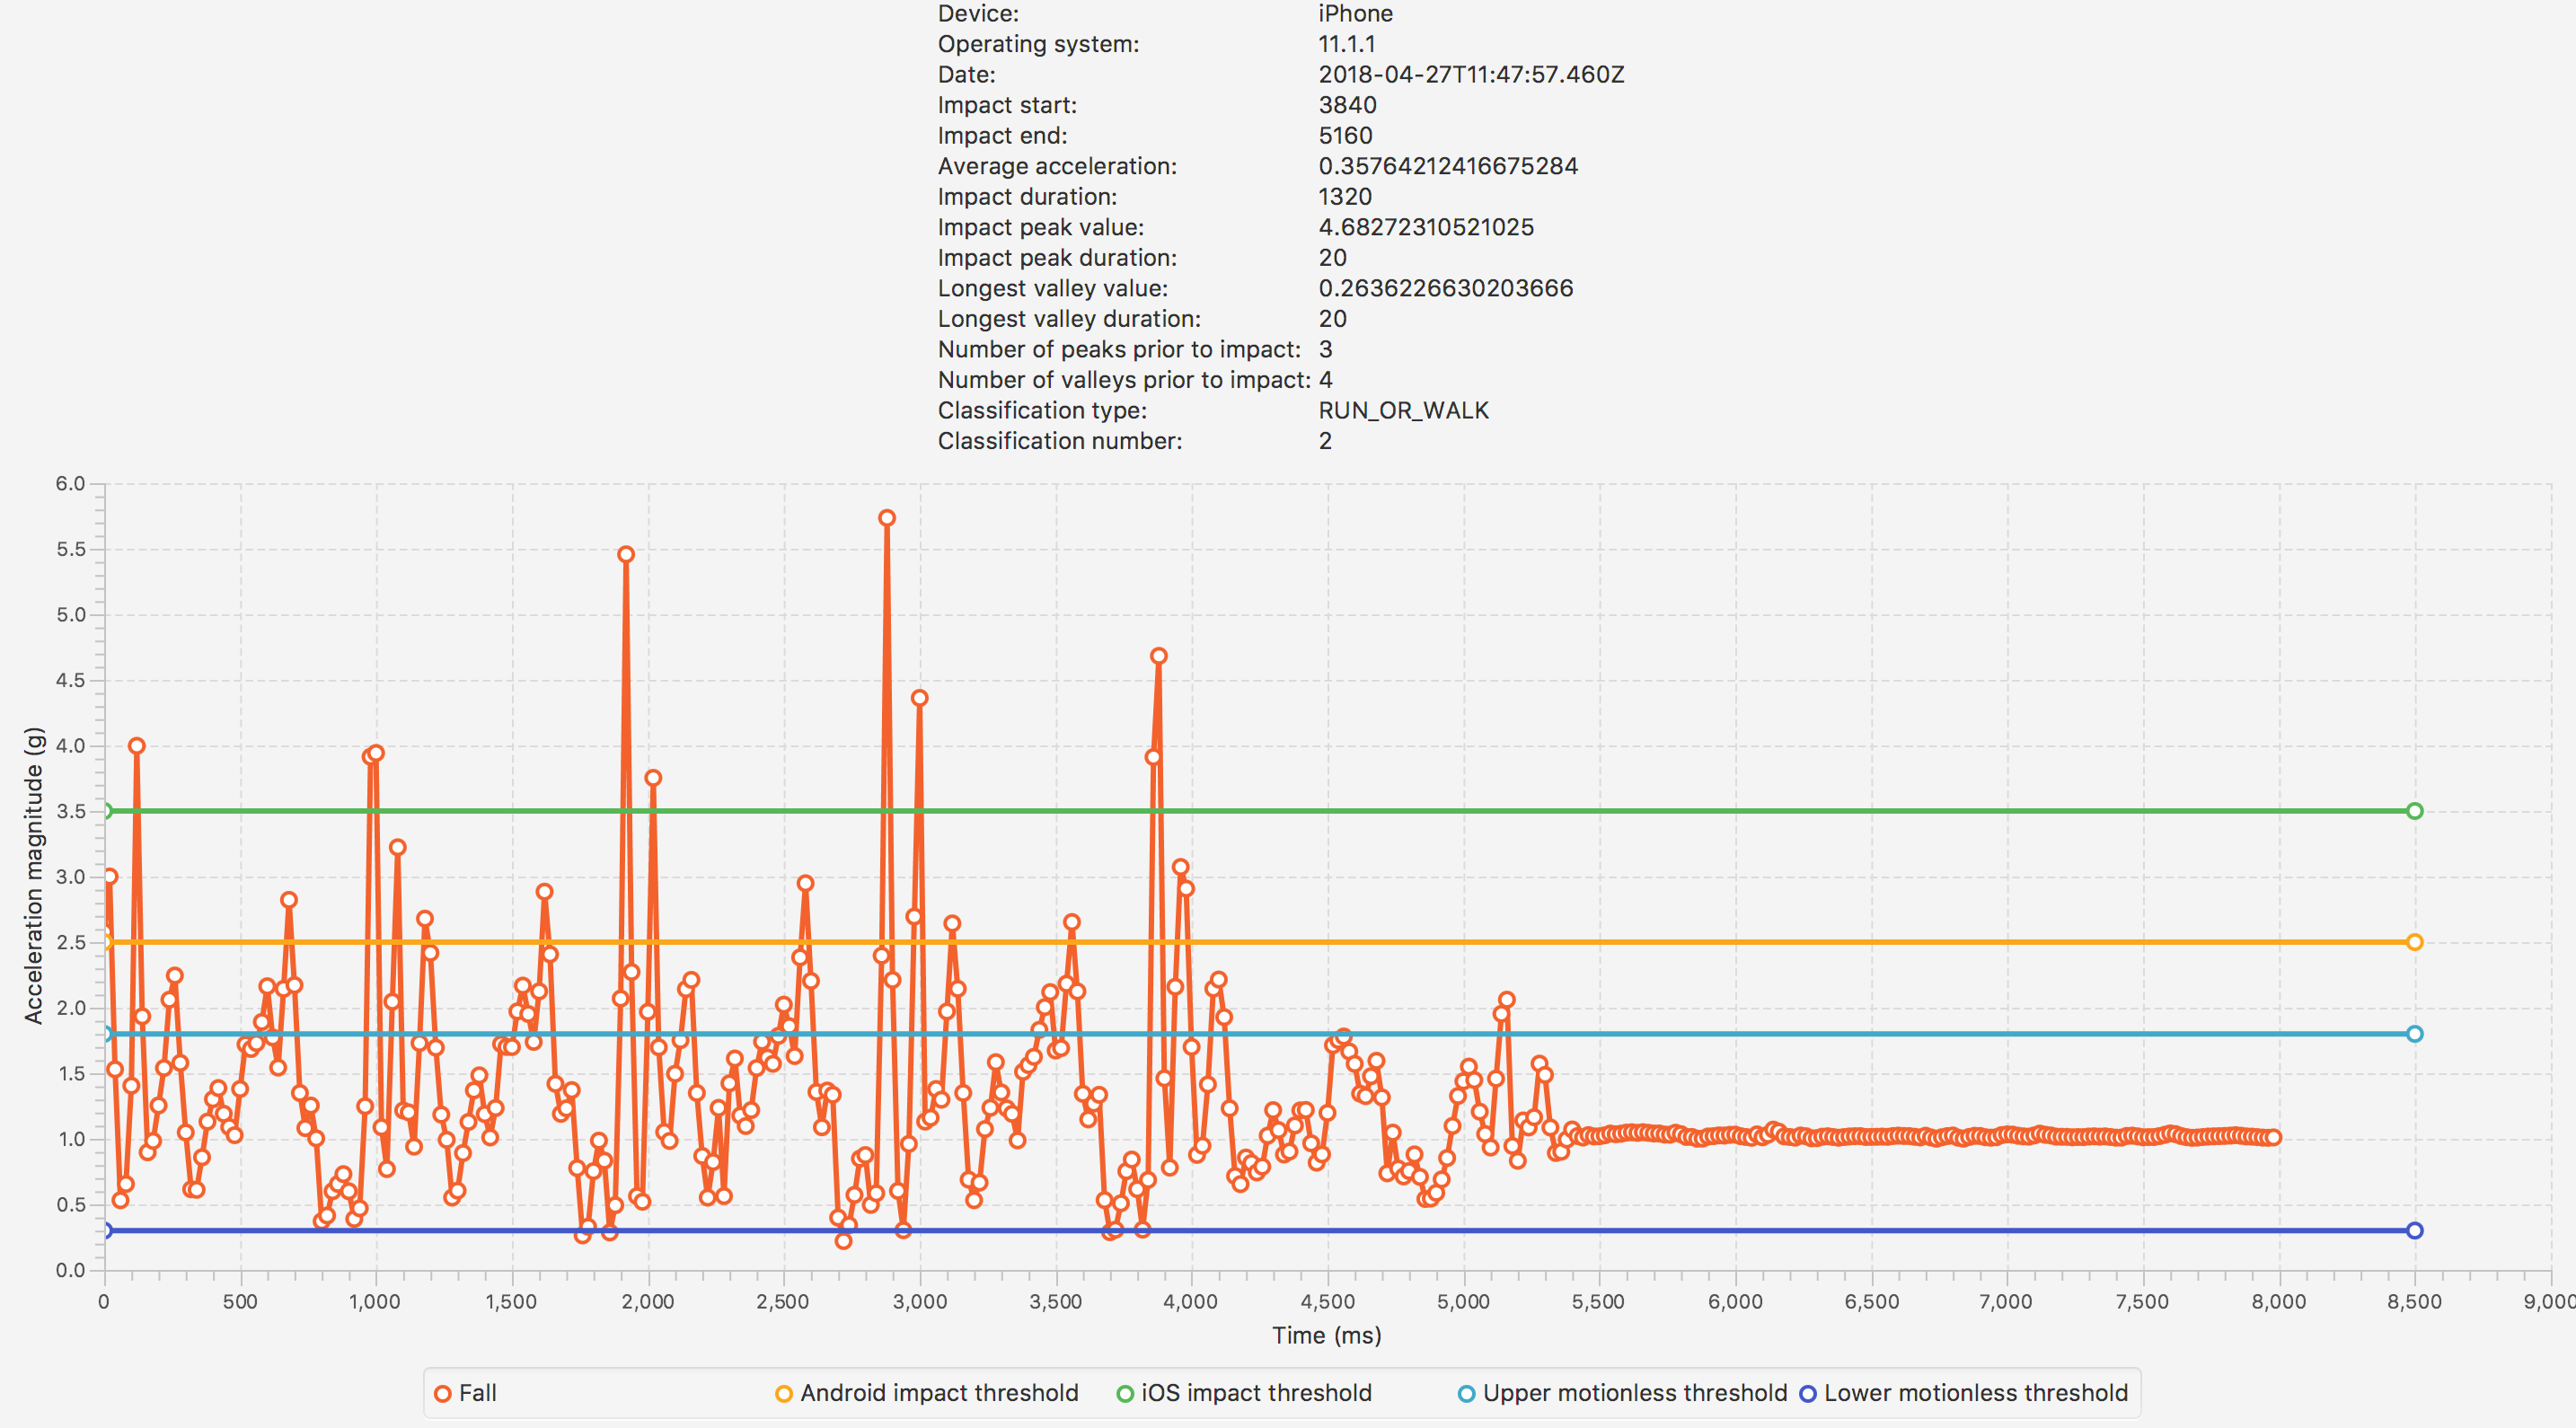
\includegraphics[width=14cm]{../img/fall-data-run-ios.png} }}%
		\caption{Recorded data on iOS while running. The acceleration variation after the peak is significant.}%
		\label{fig:fall-data-run-ios}%
	\end{figure}
	
	\begin{figure}[H]
		\centering
		\subfloat{{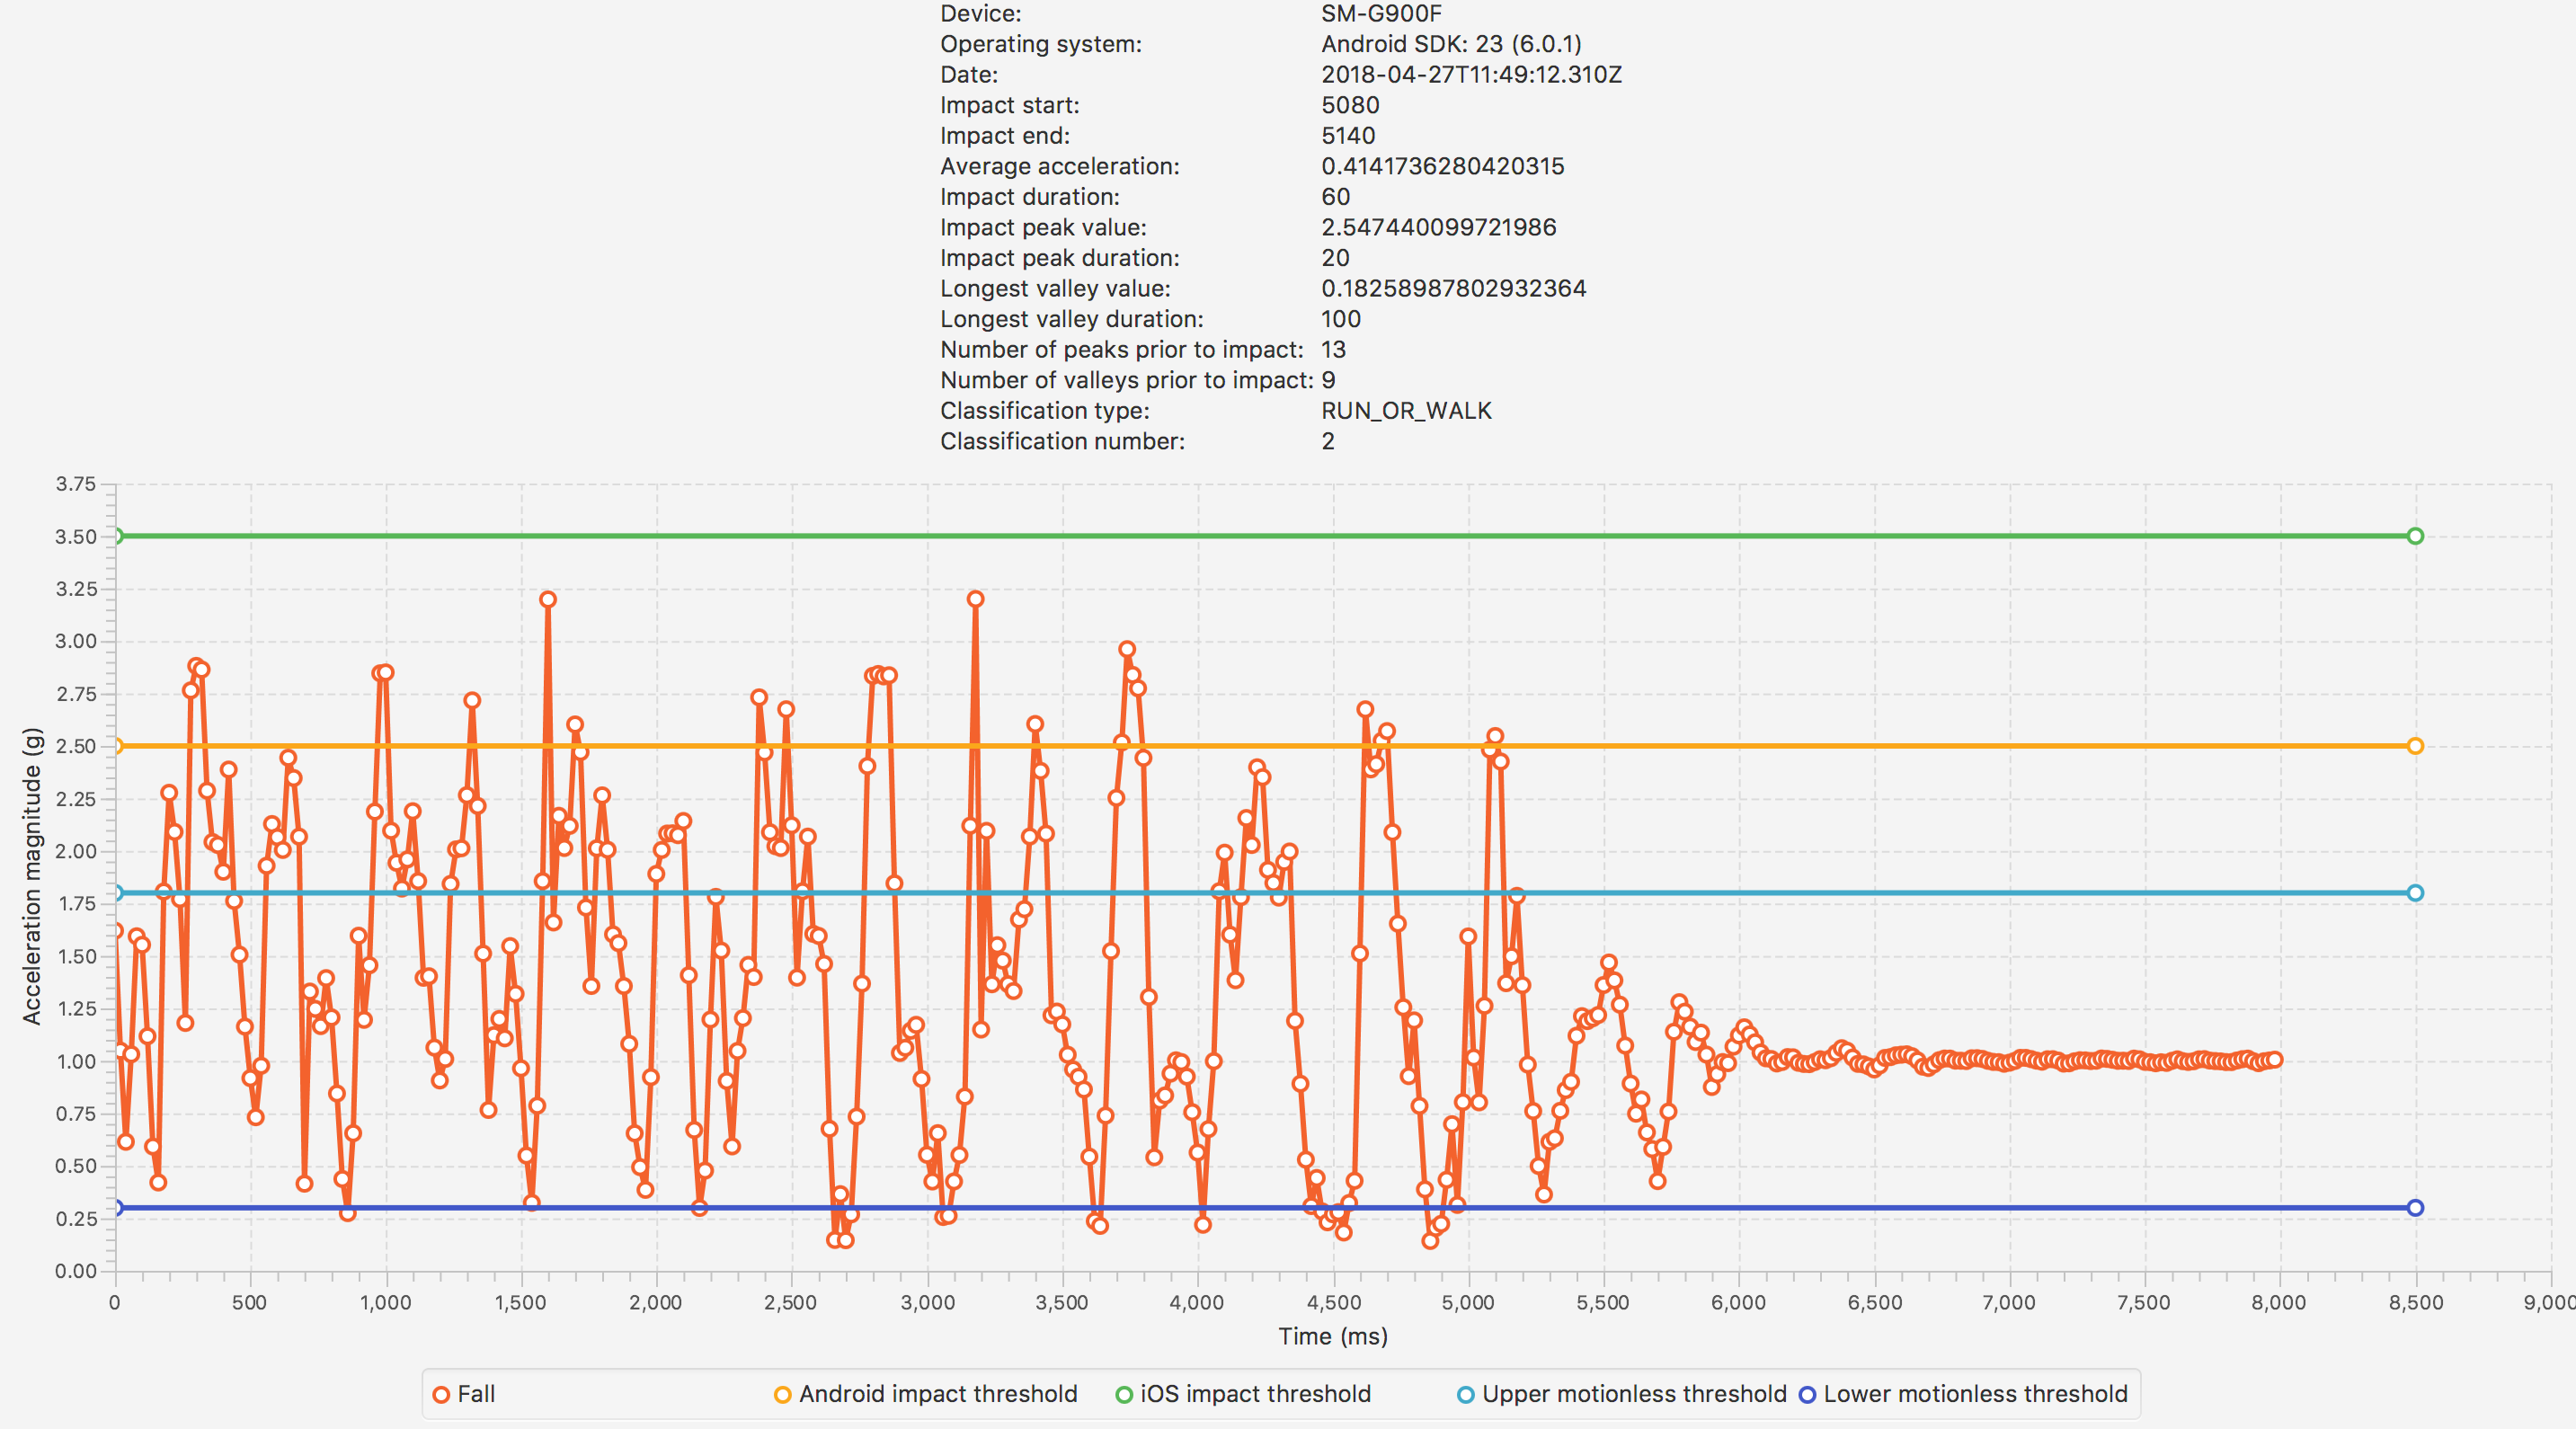
\includegraphics[width=14cm]{../img/fall-data-run-android.png} }}%
		\caption{Recorded data on Android while running. The acceleration variation after the peak is significant.}%
		\label{fig:fall-data-run-android}%
	\end{figure}
	
	\begin{figure}[H]
		\centering
		\subfloat{{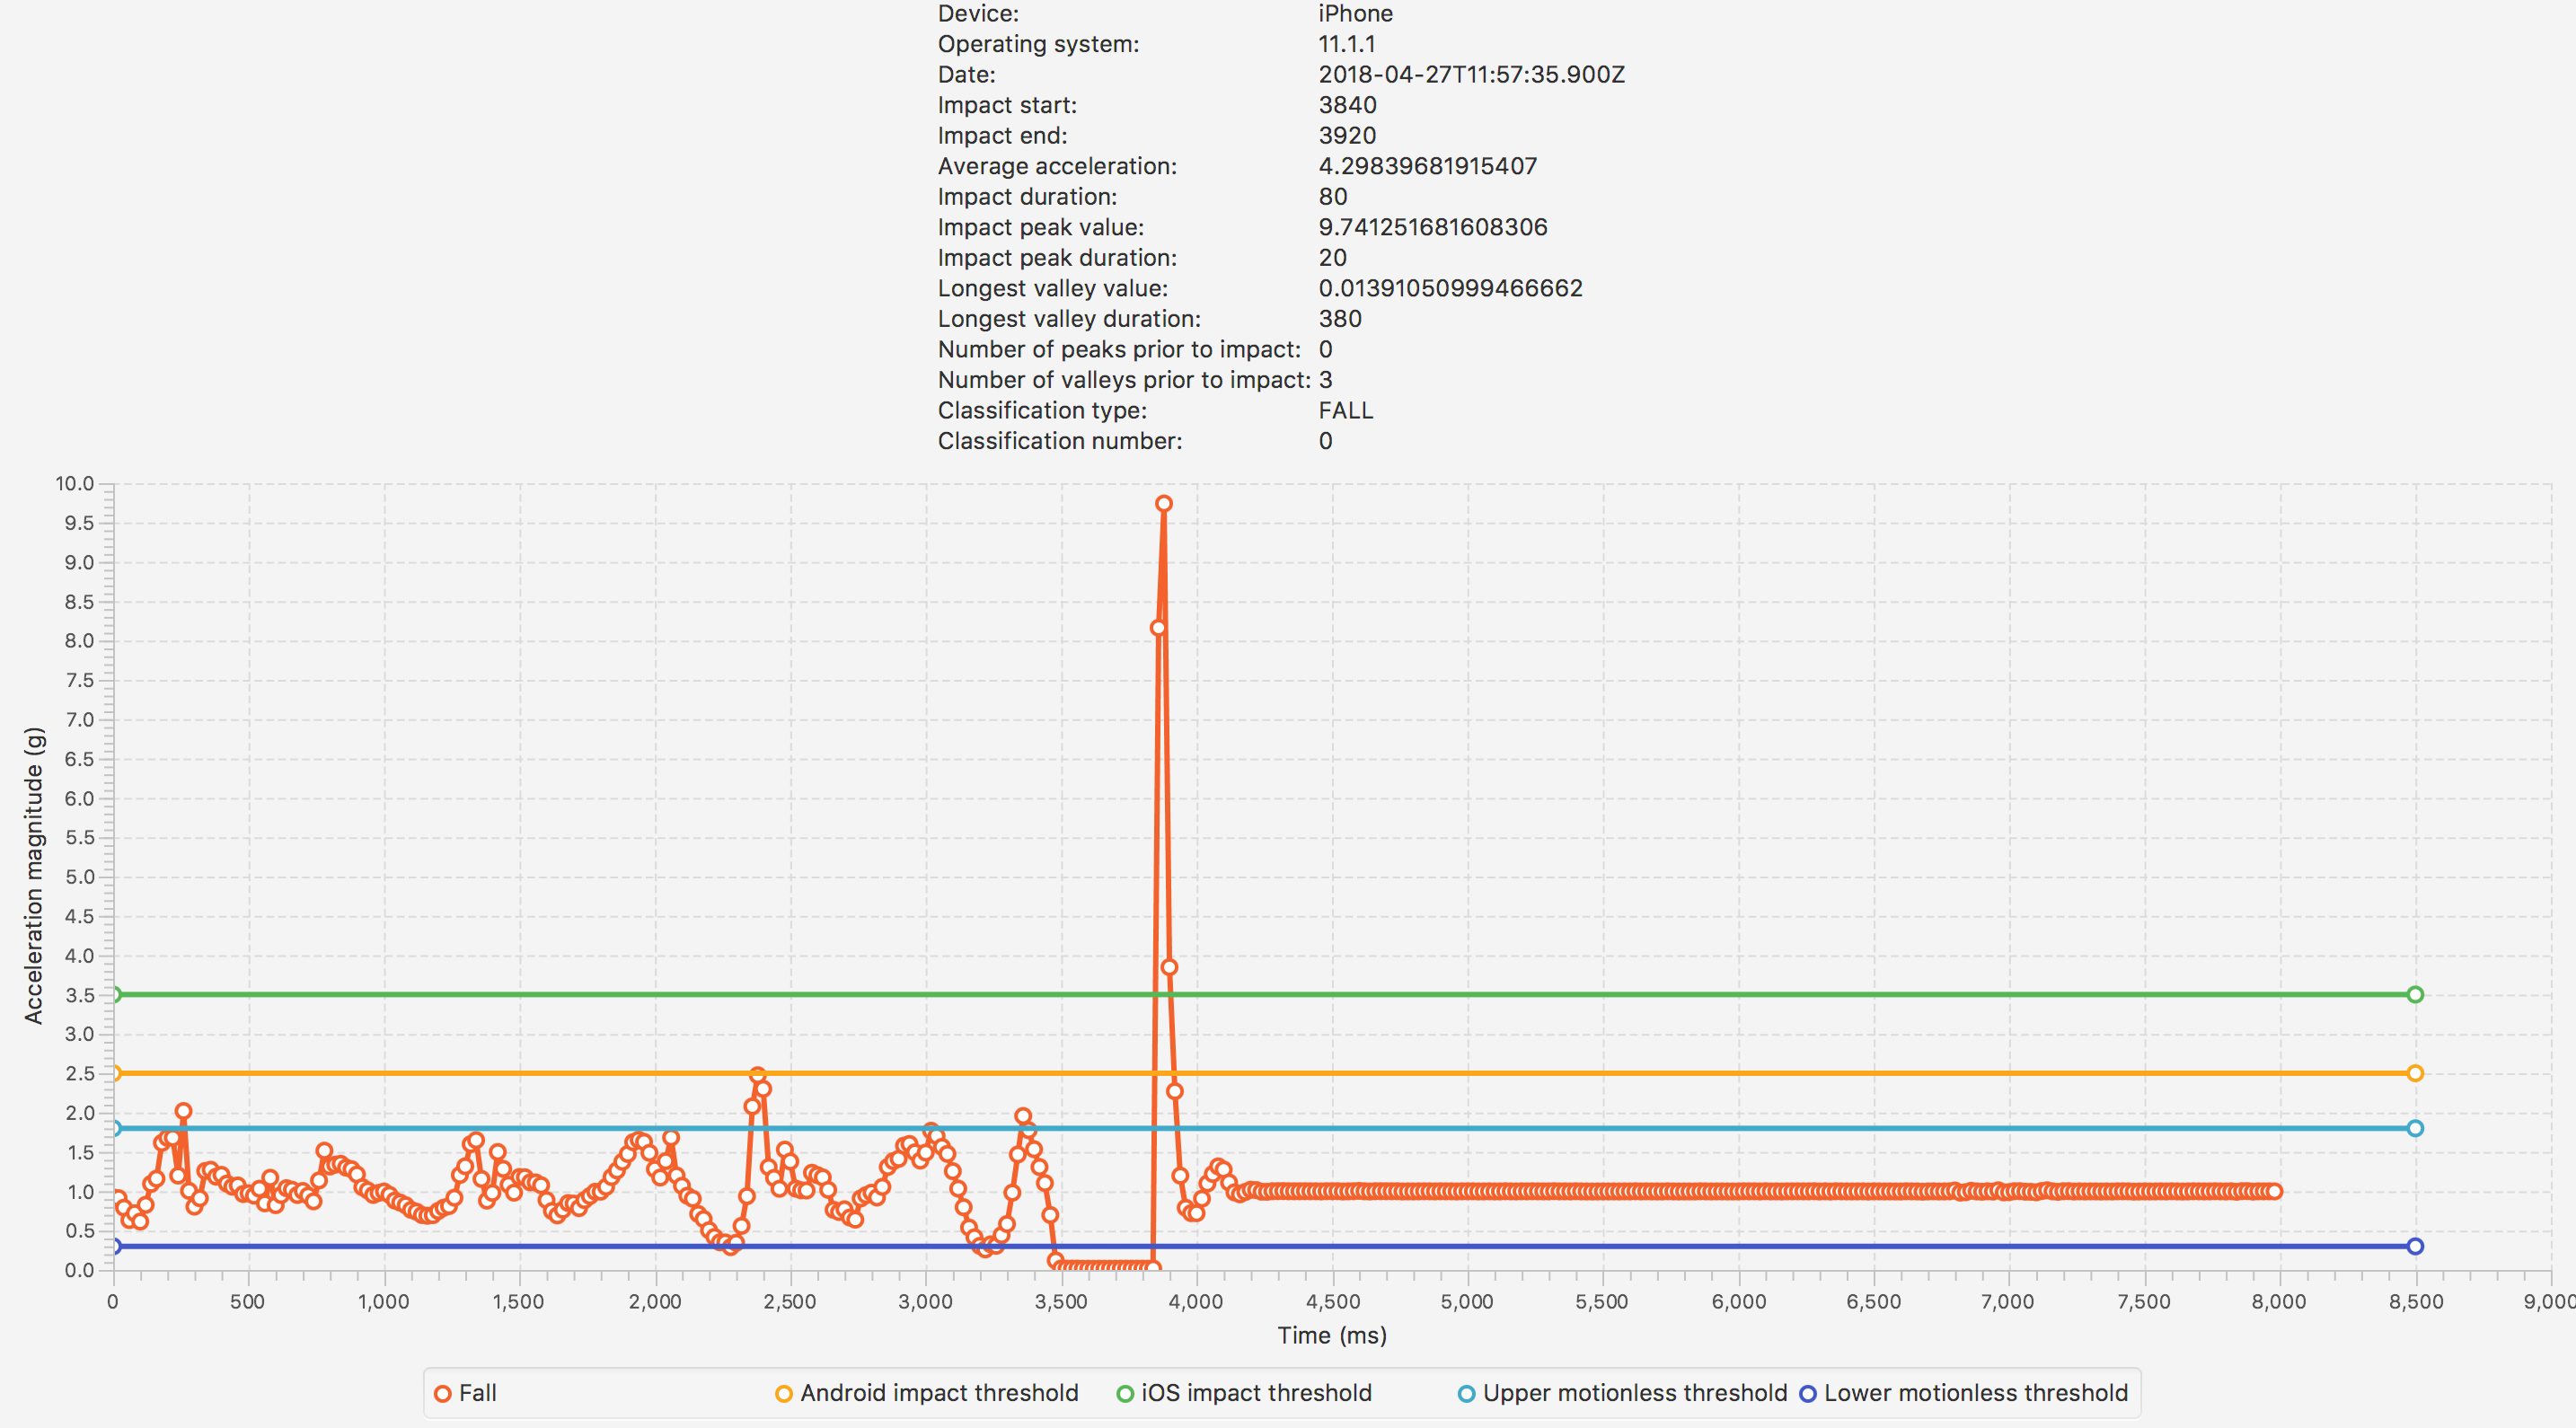
\includegraphics[width=14cm]{../img/fall-data-fall-ios.png} }}%
		\caption{Recorded data on iOS for a fall. The acceleration variation after the peak is small.}%
		\label{fig:fall-data-fall-ios}%
	\end{figure}
	
	
	\begin{figure}[H]
		\centering
		\subfloat{{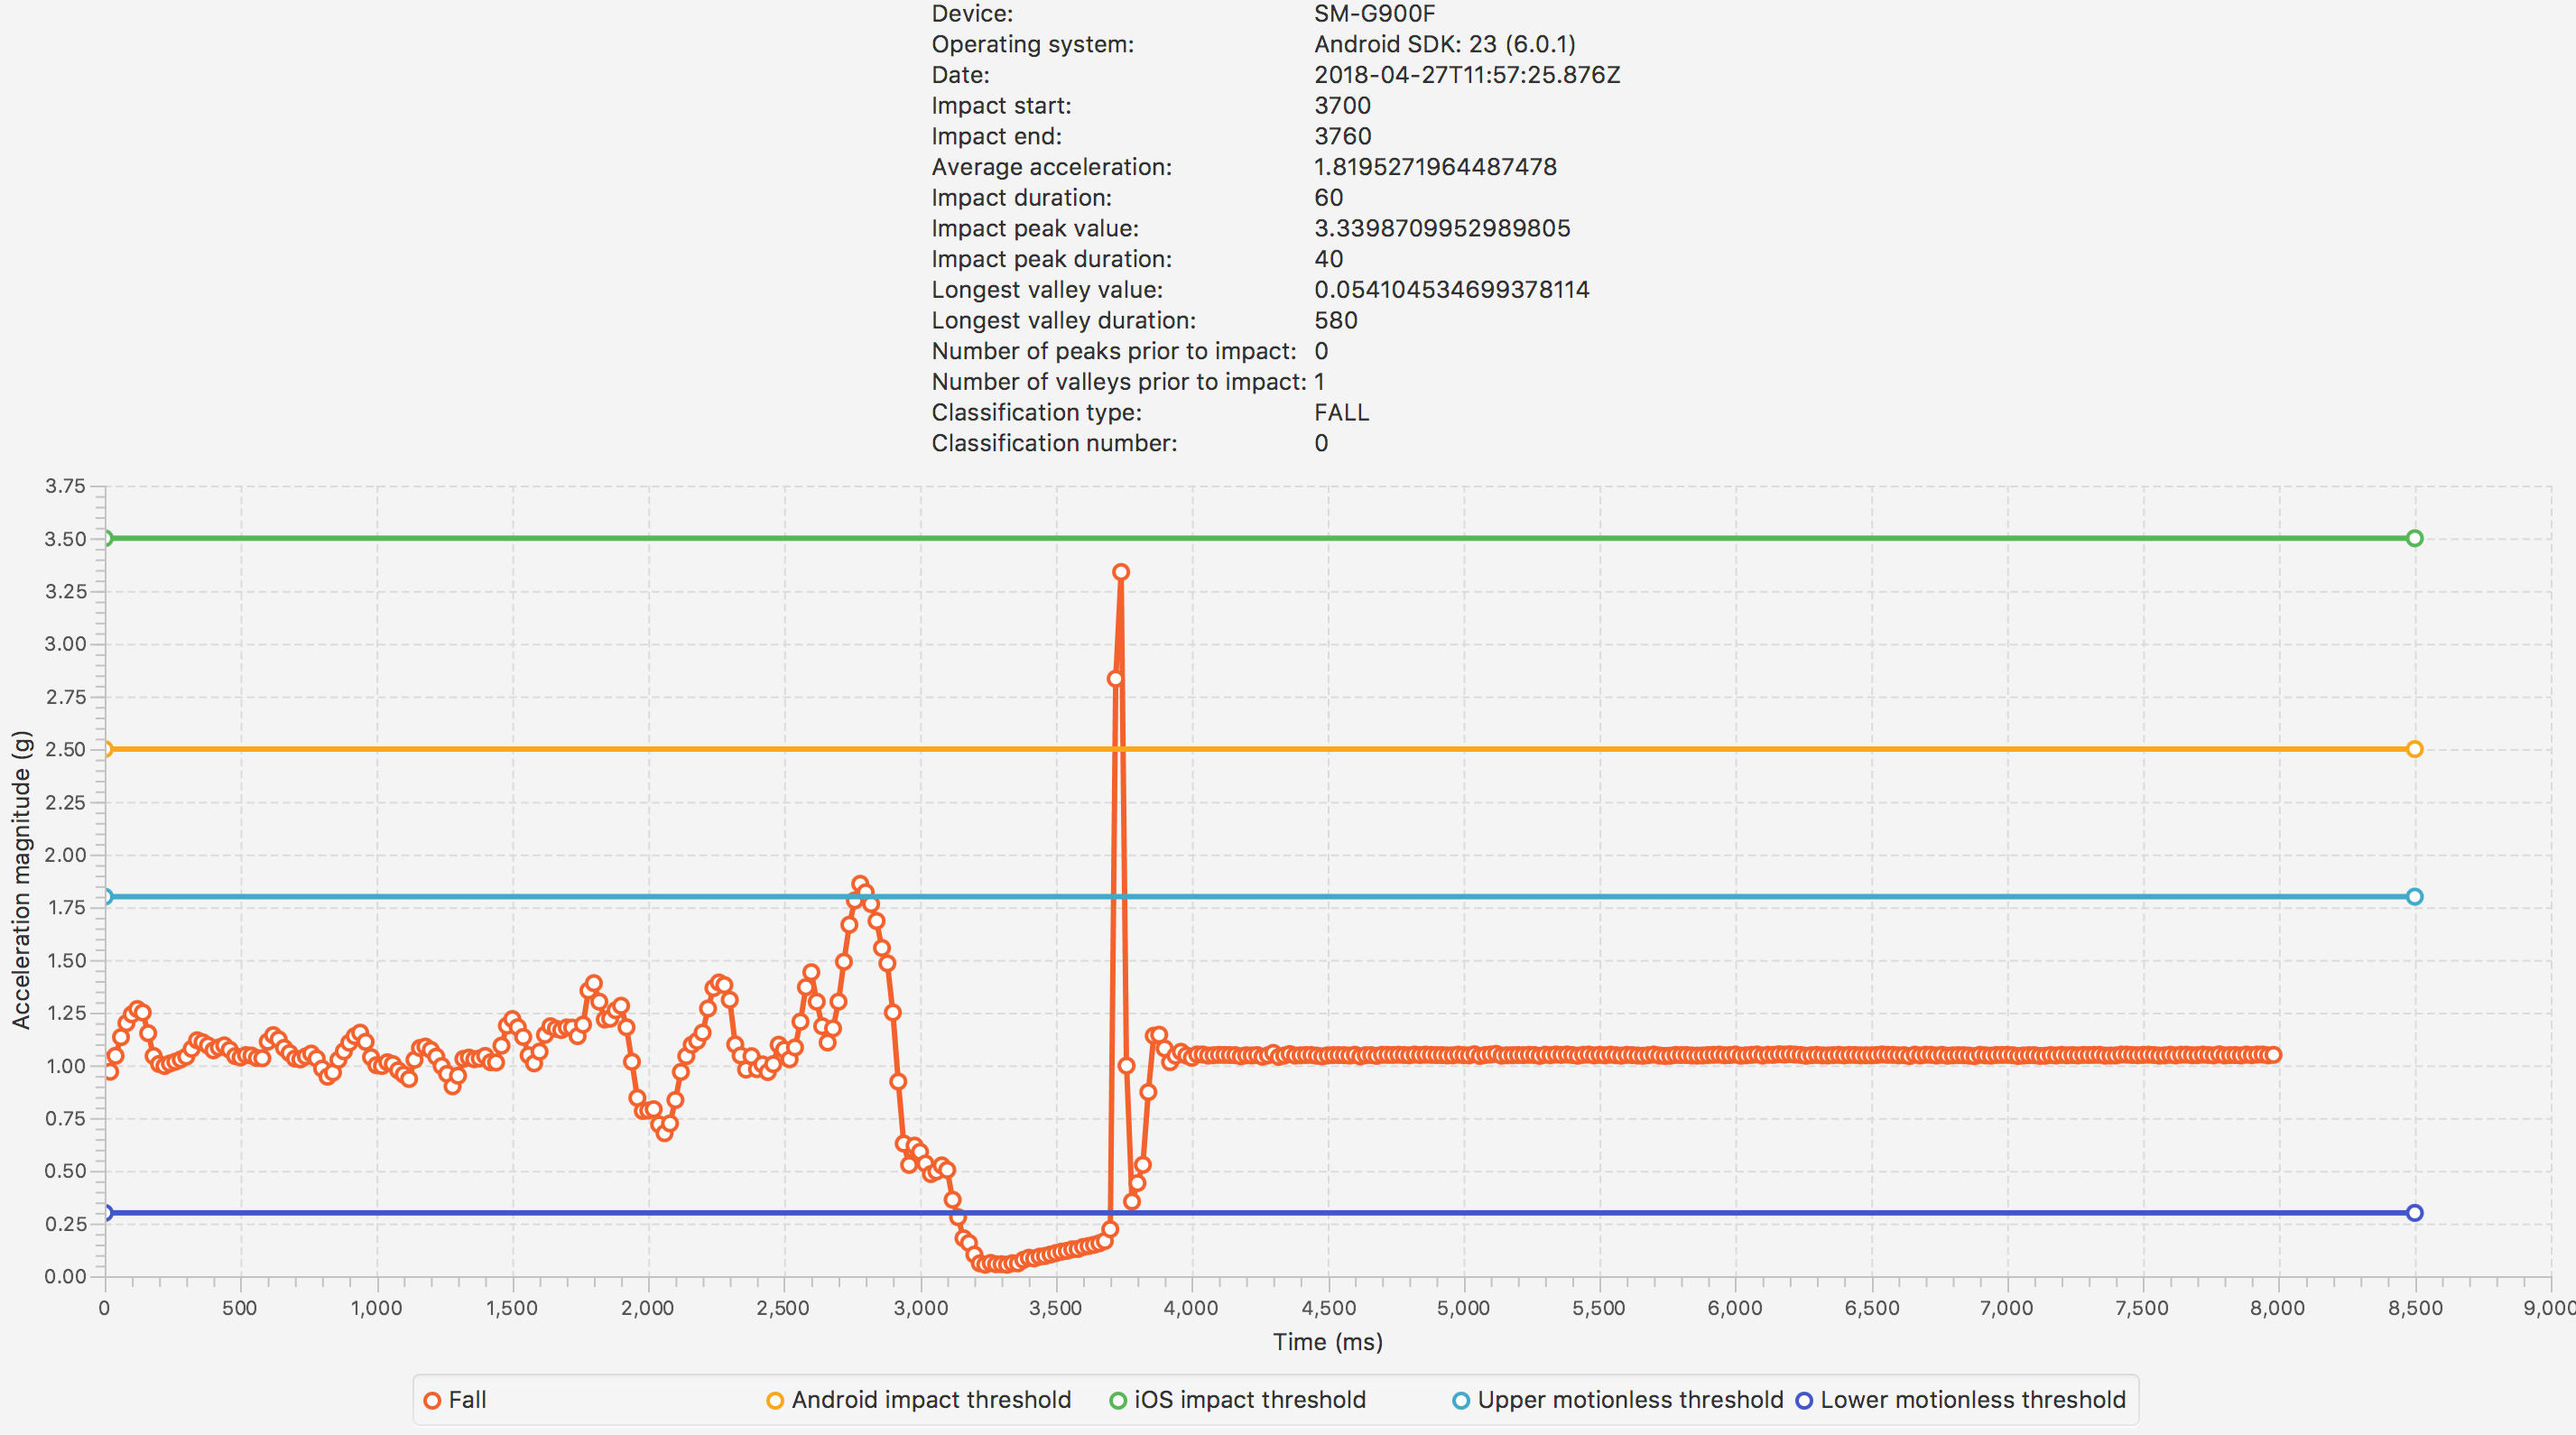
\includegraphics[width=14cm]{../img/fall-data-fall-android.png} }}%
		\caption{Recorded data on Android for a fall. The acceleration variation after the peak is small.}%
		\label{fig:fall-data-fall-android}%
	\end{figure}
	
	
	
	\subsubsection{Impact duration}
	
	The impact duration is the time in milliseconds elapsed from the first sample of the impact peak exceeding the impact threshold to the last sample that is outside of the interval [Lower motionless threshold, Upper motionless threshold]. An example of impact duration is highlighted in figure \ref{fig:fall-data-impact-duration}.
	
	
	\begin{figure}[H]
		\centering
		\subfloat{{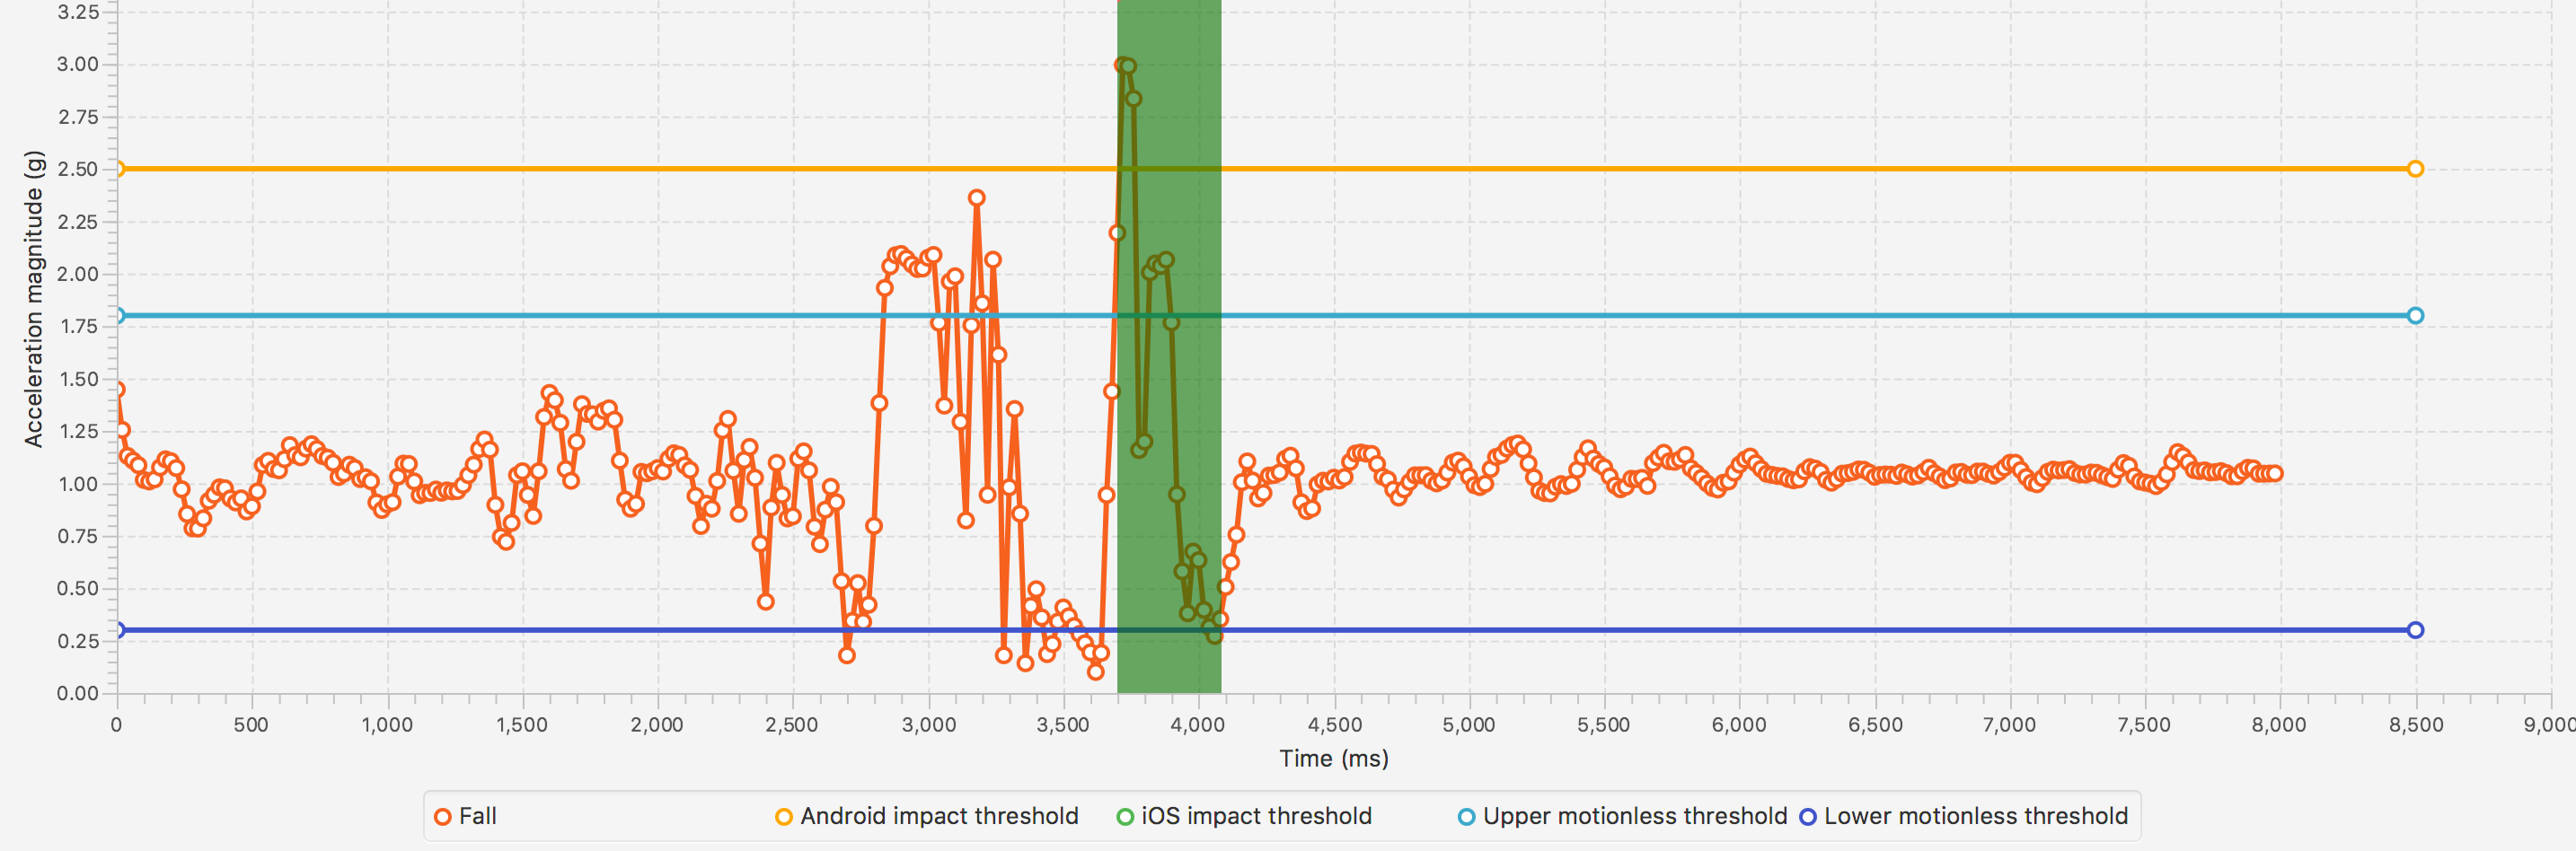
\includegraphics[width=14cm]{../img/fall-data-impact-duration-android-highlight.png} }}%
		\caption{Visualization of impact duration. The impact duration is highlighted in green. The impact start is around 3700 ms and impact end around 4080 ms, which gives an impact duration of \textit{4080 - 3700 = 380 ms}.}%
		\label{fig:fall-data-impact-duration}%
	\end{figure}
	
	\subsubsection{Impact peak value}
	
	The impact peak value is the highest value for acceleration vector length found on the last peak. The last peak is the peak that triggered the state machine. An example of impact peak value is highlighted in figure \ref{fig:fall-data-impact-peak}.
	
	\begin{figure}[H]
		\centering
		\subfloat{{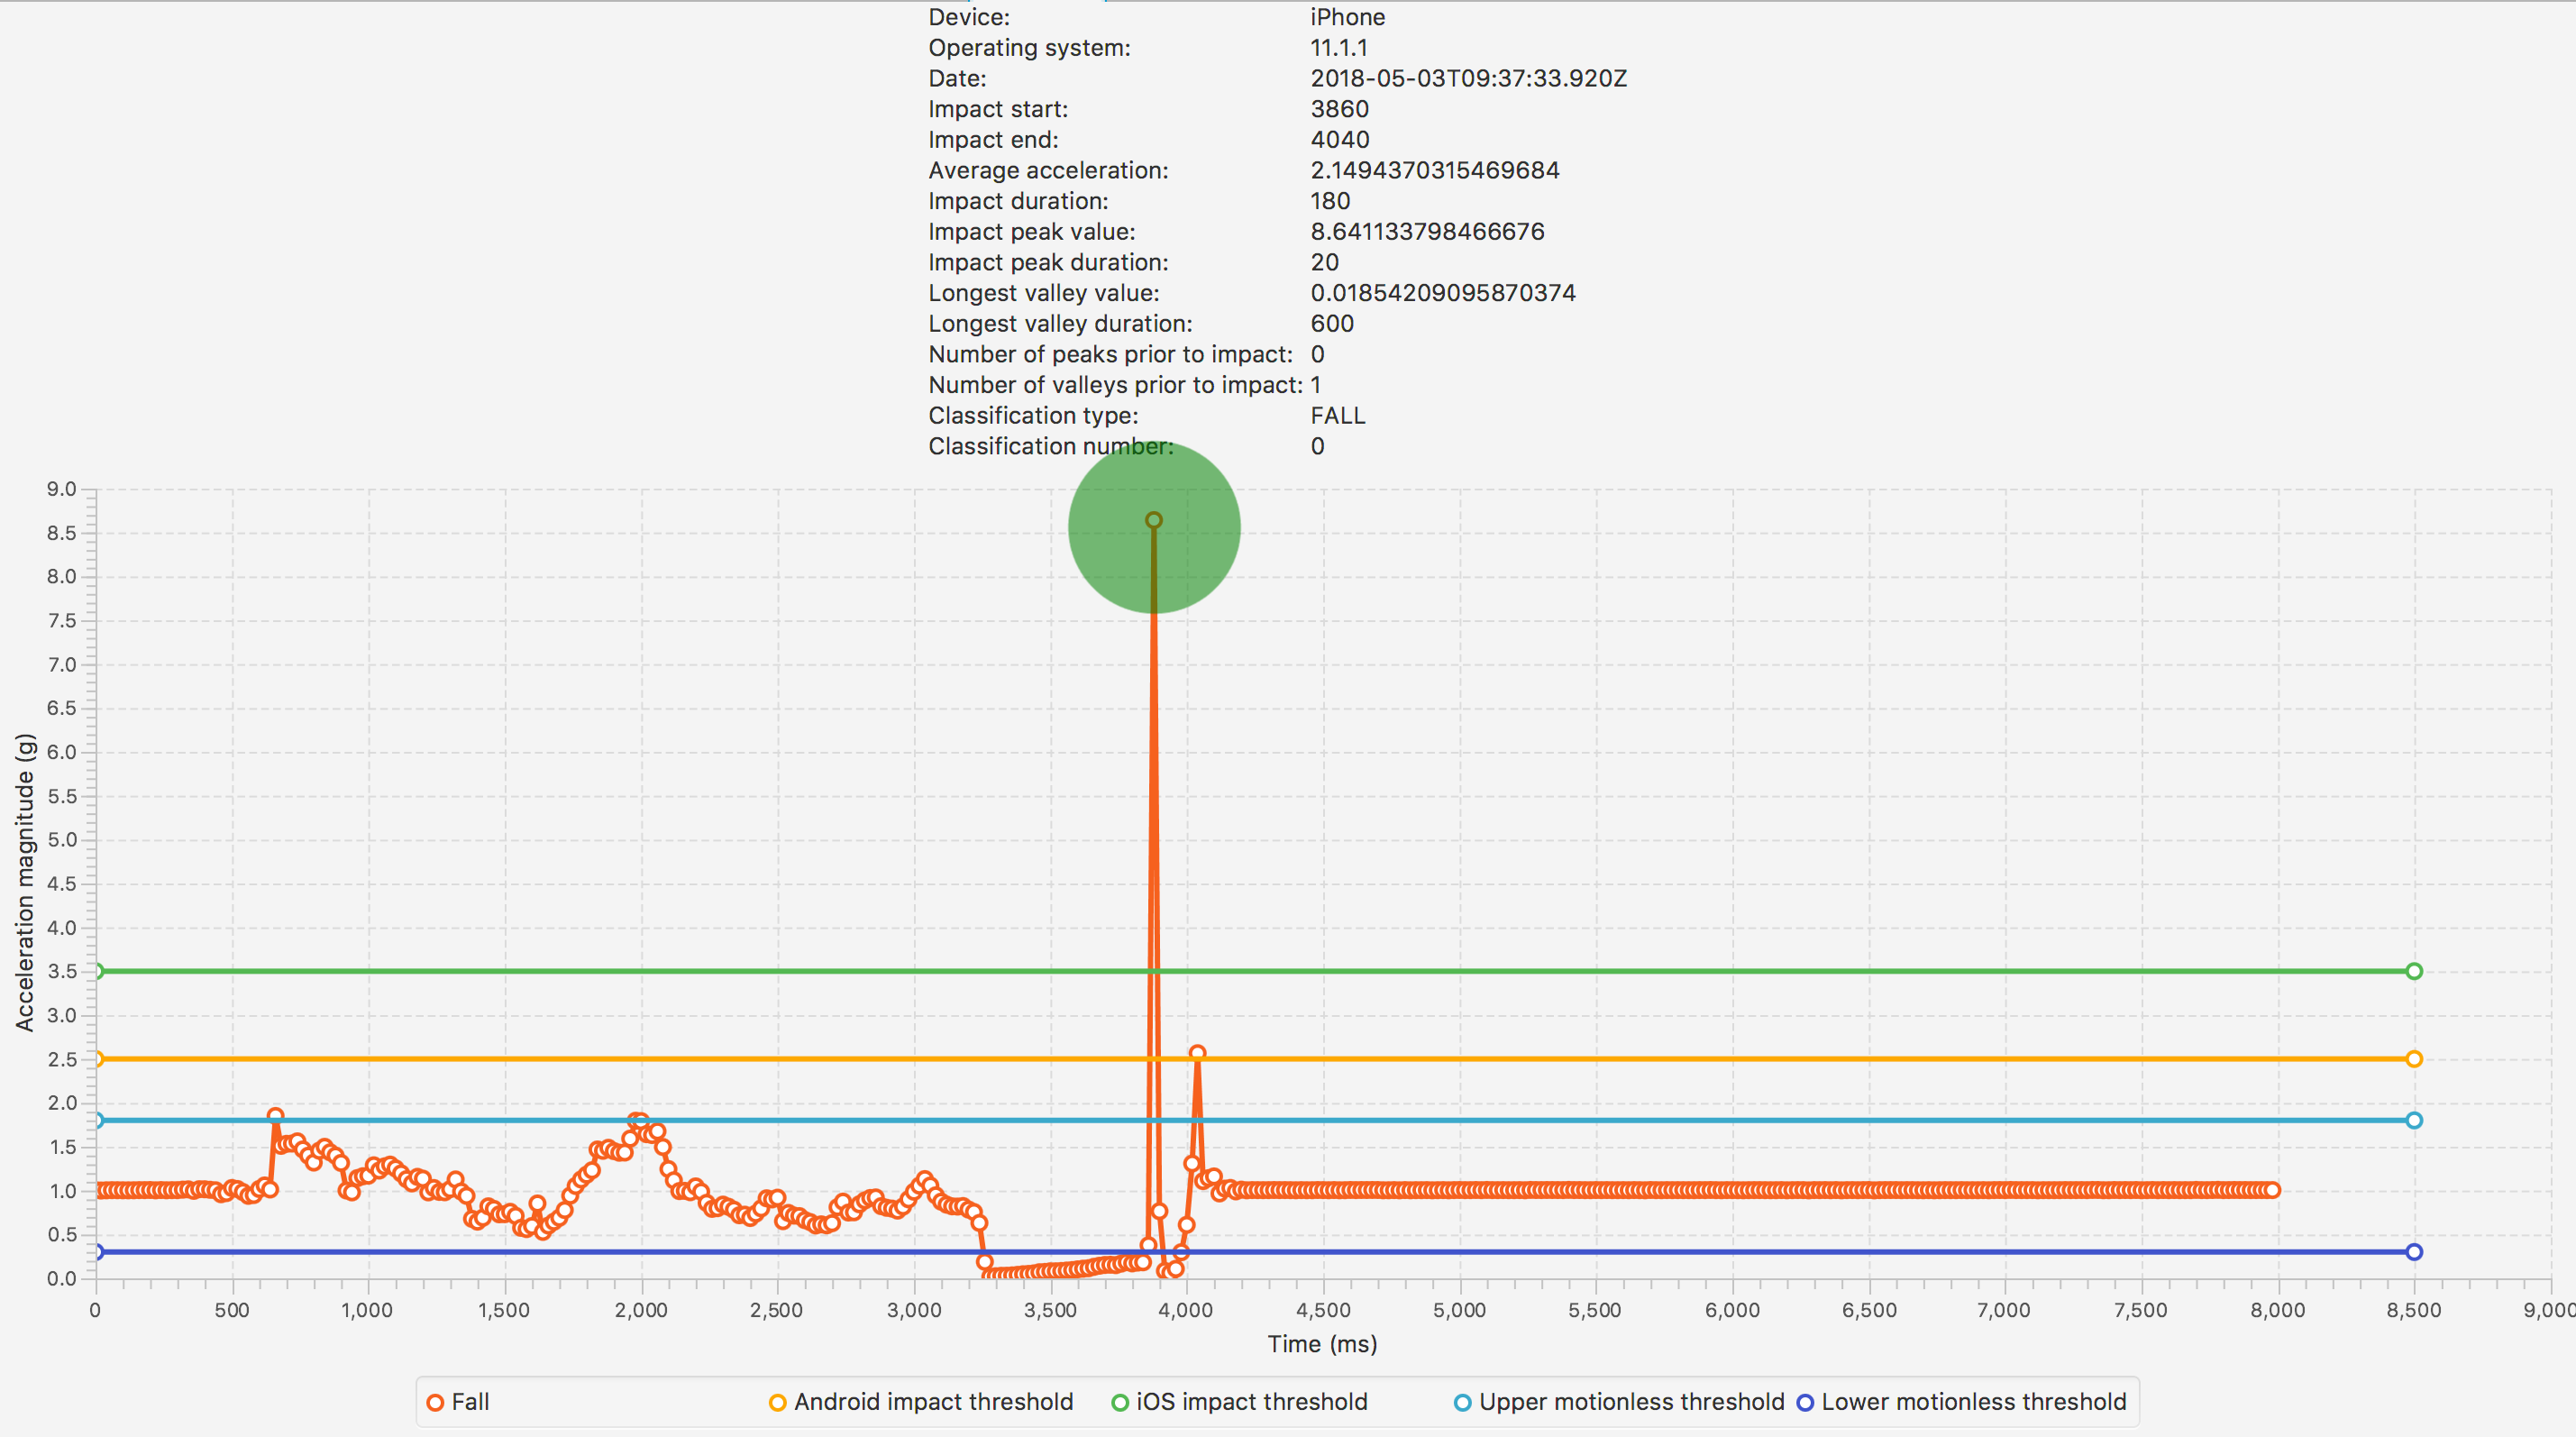
\includegraphics[width=14cm]{../img/fall-data-impact-peak-highlight.png} }}%
		\caption{Visualization of impact peak value. This fall has a significant impact peak value of around \textit{8.6g}}%
		\label{fig:fall-data-impact-peak}%
	\end{figure}
	
	\subsubsection{Impact peak duration}
	
	The impact peak duration is the time in ms that the last peak exceeds the impact threshold. An example of this is shown in figure \ref{fig:fall-data-impact-peak-duration}.
	
	\begin{figure}[H]
		\centering
		\subfloat{{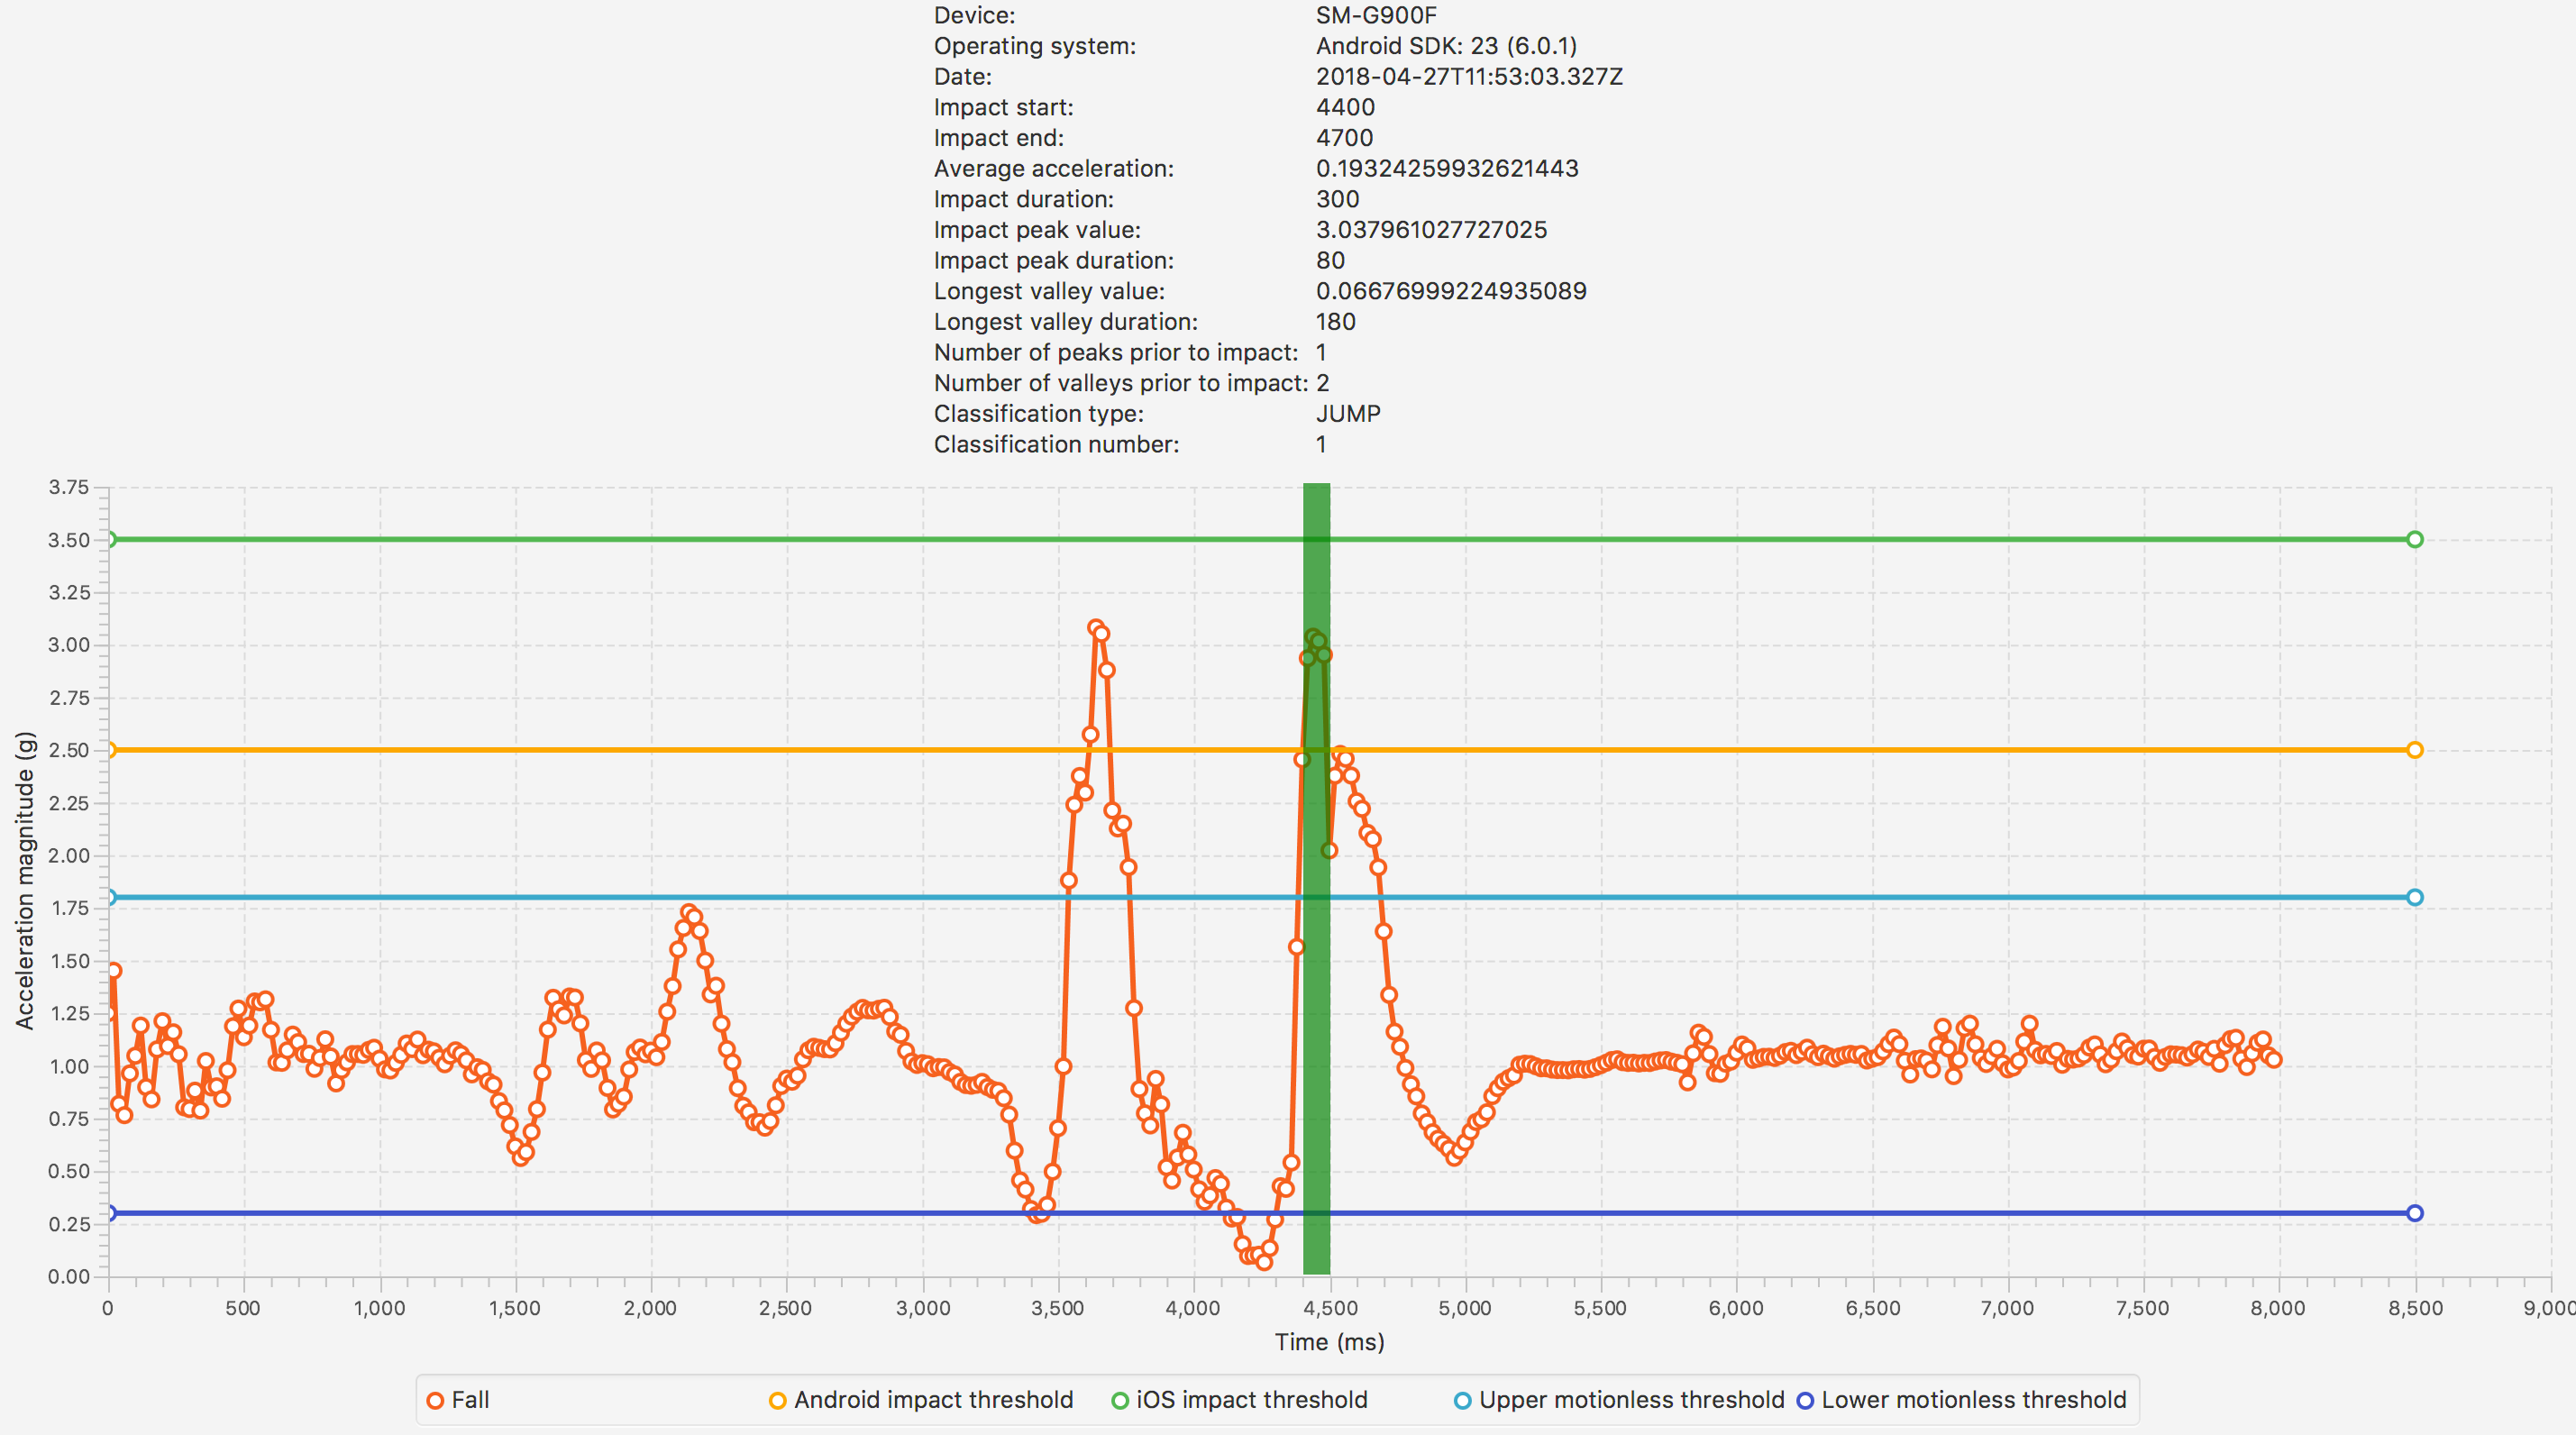
\includegraphics[width=14cm]{../img/fall-data-impact-peak-duration-highlight.png} }}%
		\caption{Visualization of impact peak duration. The impact peak duration is highlighted in green.}%
		\label{fig:fall-data-impact-peak-duration}%
	\end{figure}
	
	\subsubsection{Longest valley value}
	
	The longest valley is the longest continuous time found where each sample is below the lower motionless threshold. The longest valley value is the lowest sampling value found during that time. An example of longest valley value is shown in figure \ref{fig:fall-data-longest-valley-value}
	
	\begin{figure}[H]
		\centering
		\subfloat{{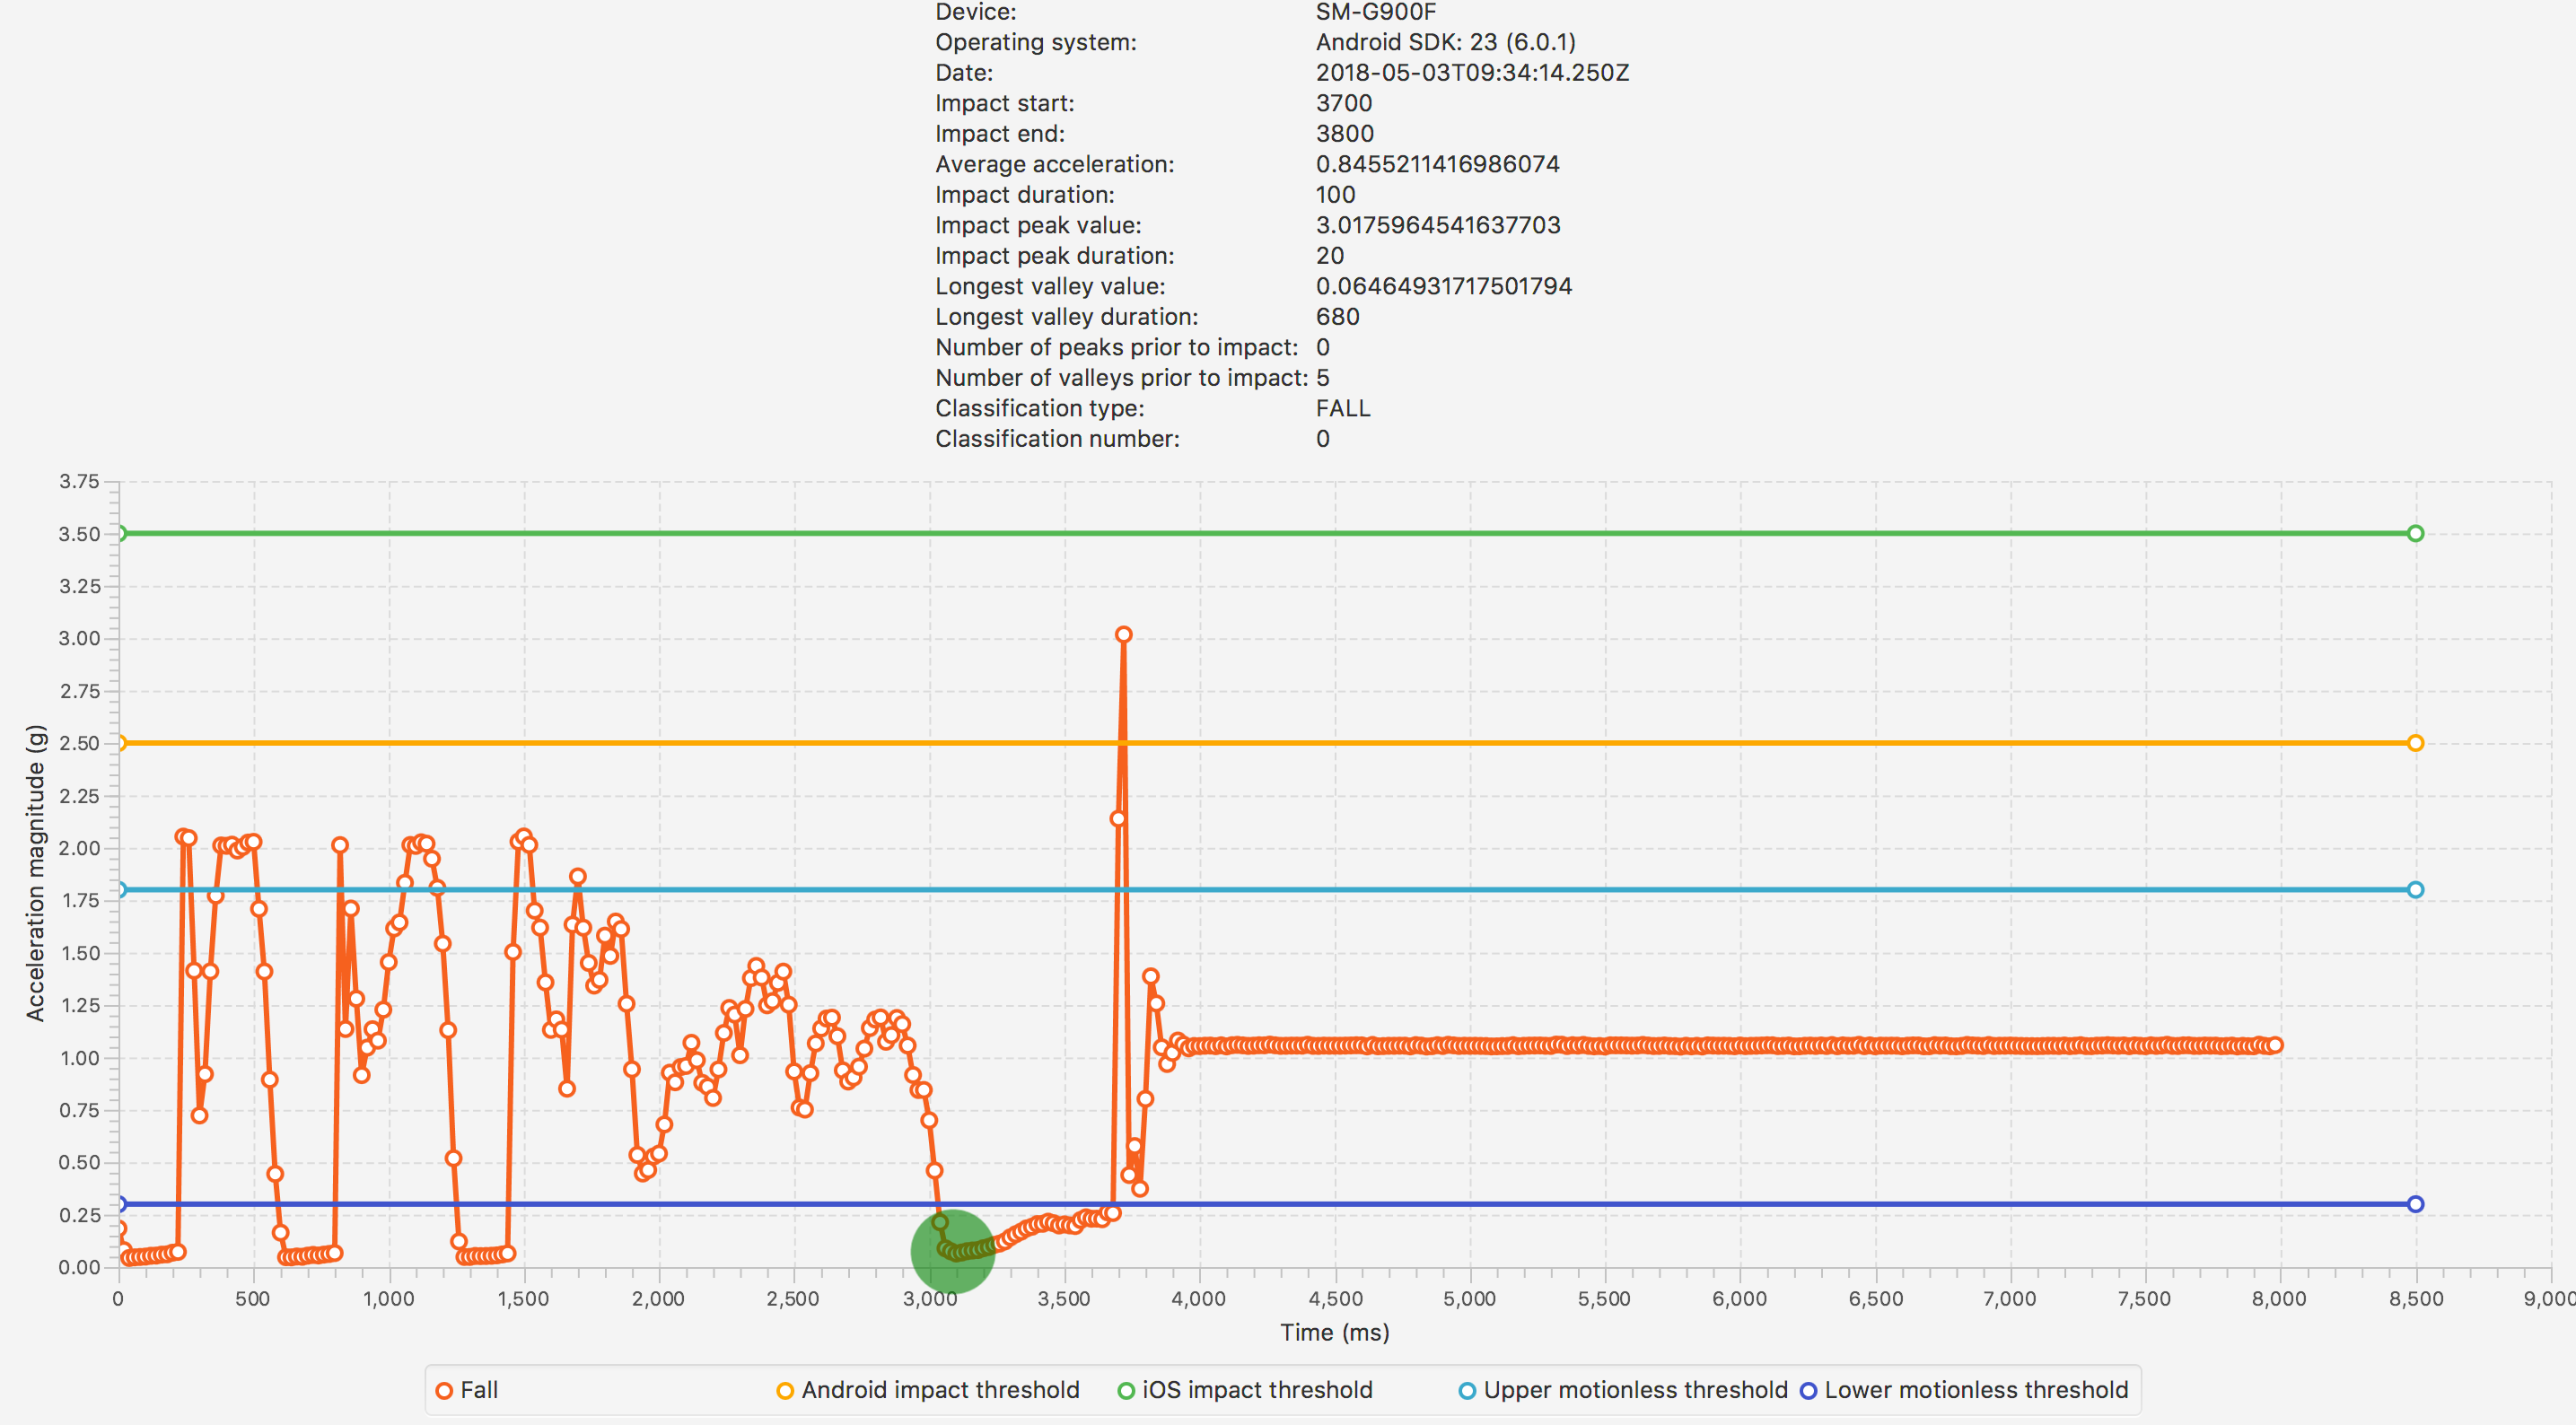
\includegraphics[width=14cm]{../img/fall-data-longest-valley-value-highlight.png} }}%
		\caption{Visualization of longest valley value. The longest valley value is highlighted in green.}%
		\label{fig:fall-data-longest-valley-value}%
	\end{figure}
	
	\subsubsection{Longest valley duration}
	
	The longest valley is the same as described in longest valley value. The longest valley duration is the time in milliseconds elapsed during this interval. The time period for longest valley duration is highlighted in figure \ref{fig:fall-data-longest-valley-duration}.
	
	\begin{figure}[H]
		\centering
		\subfloat{{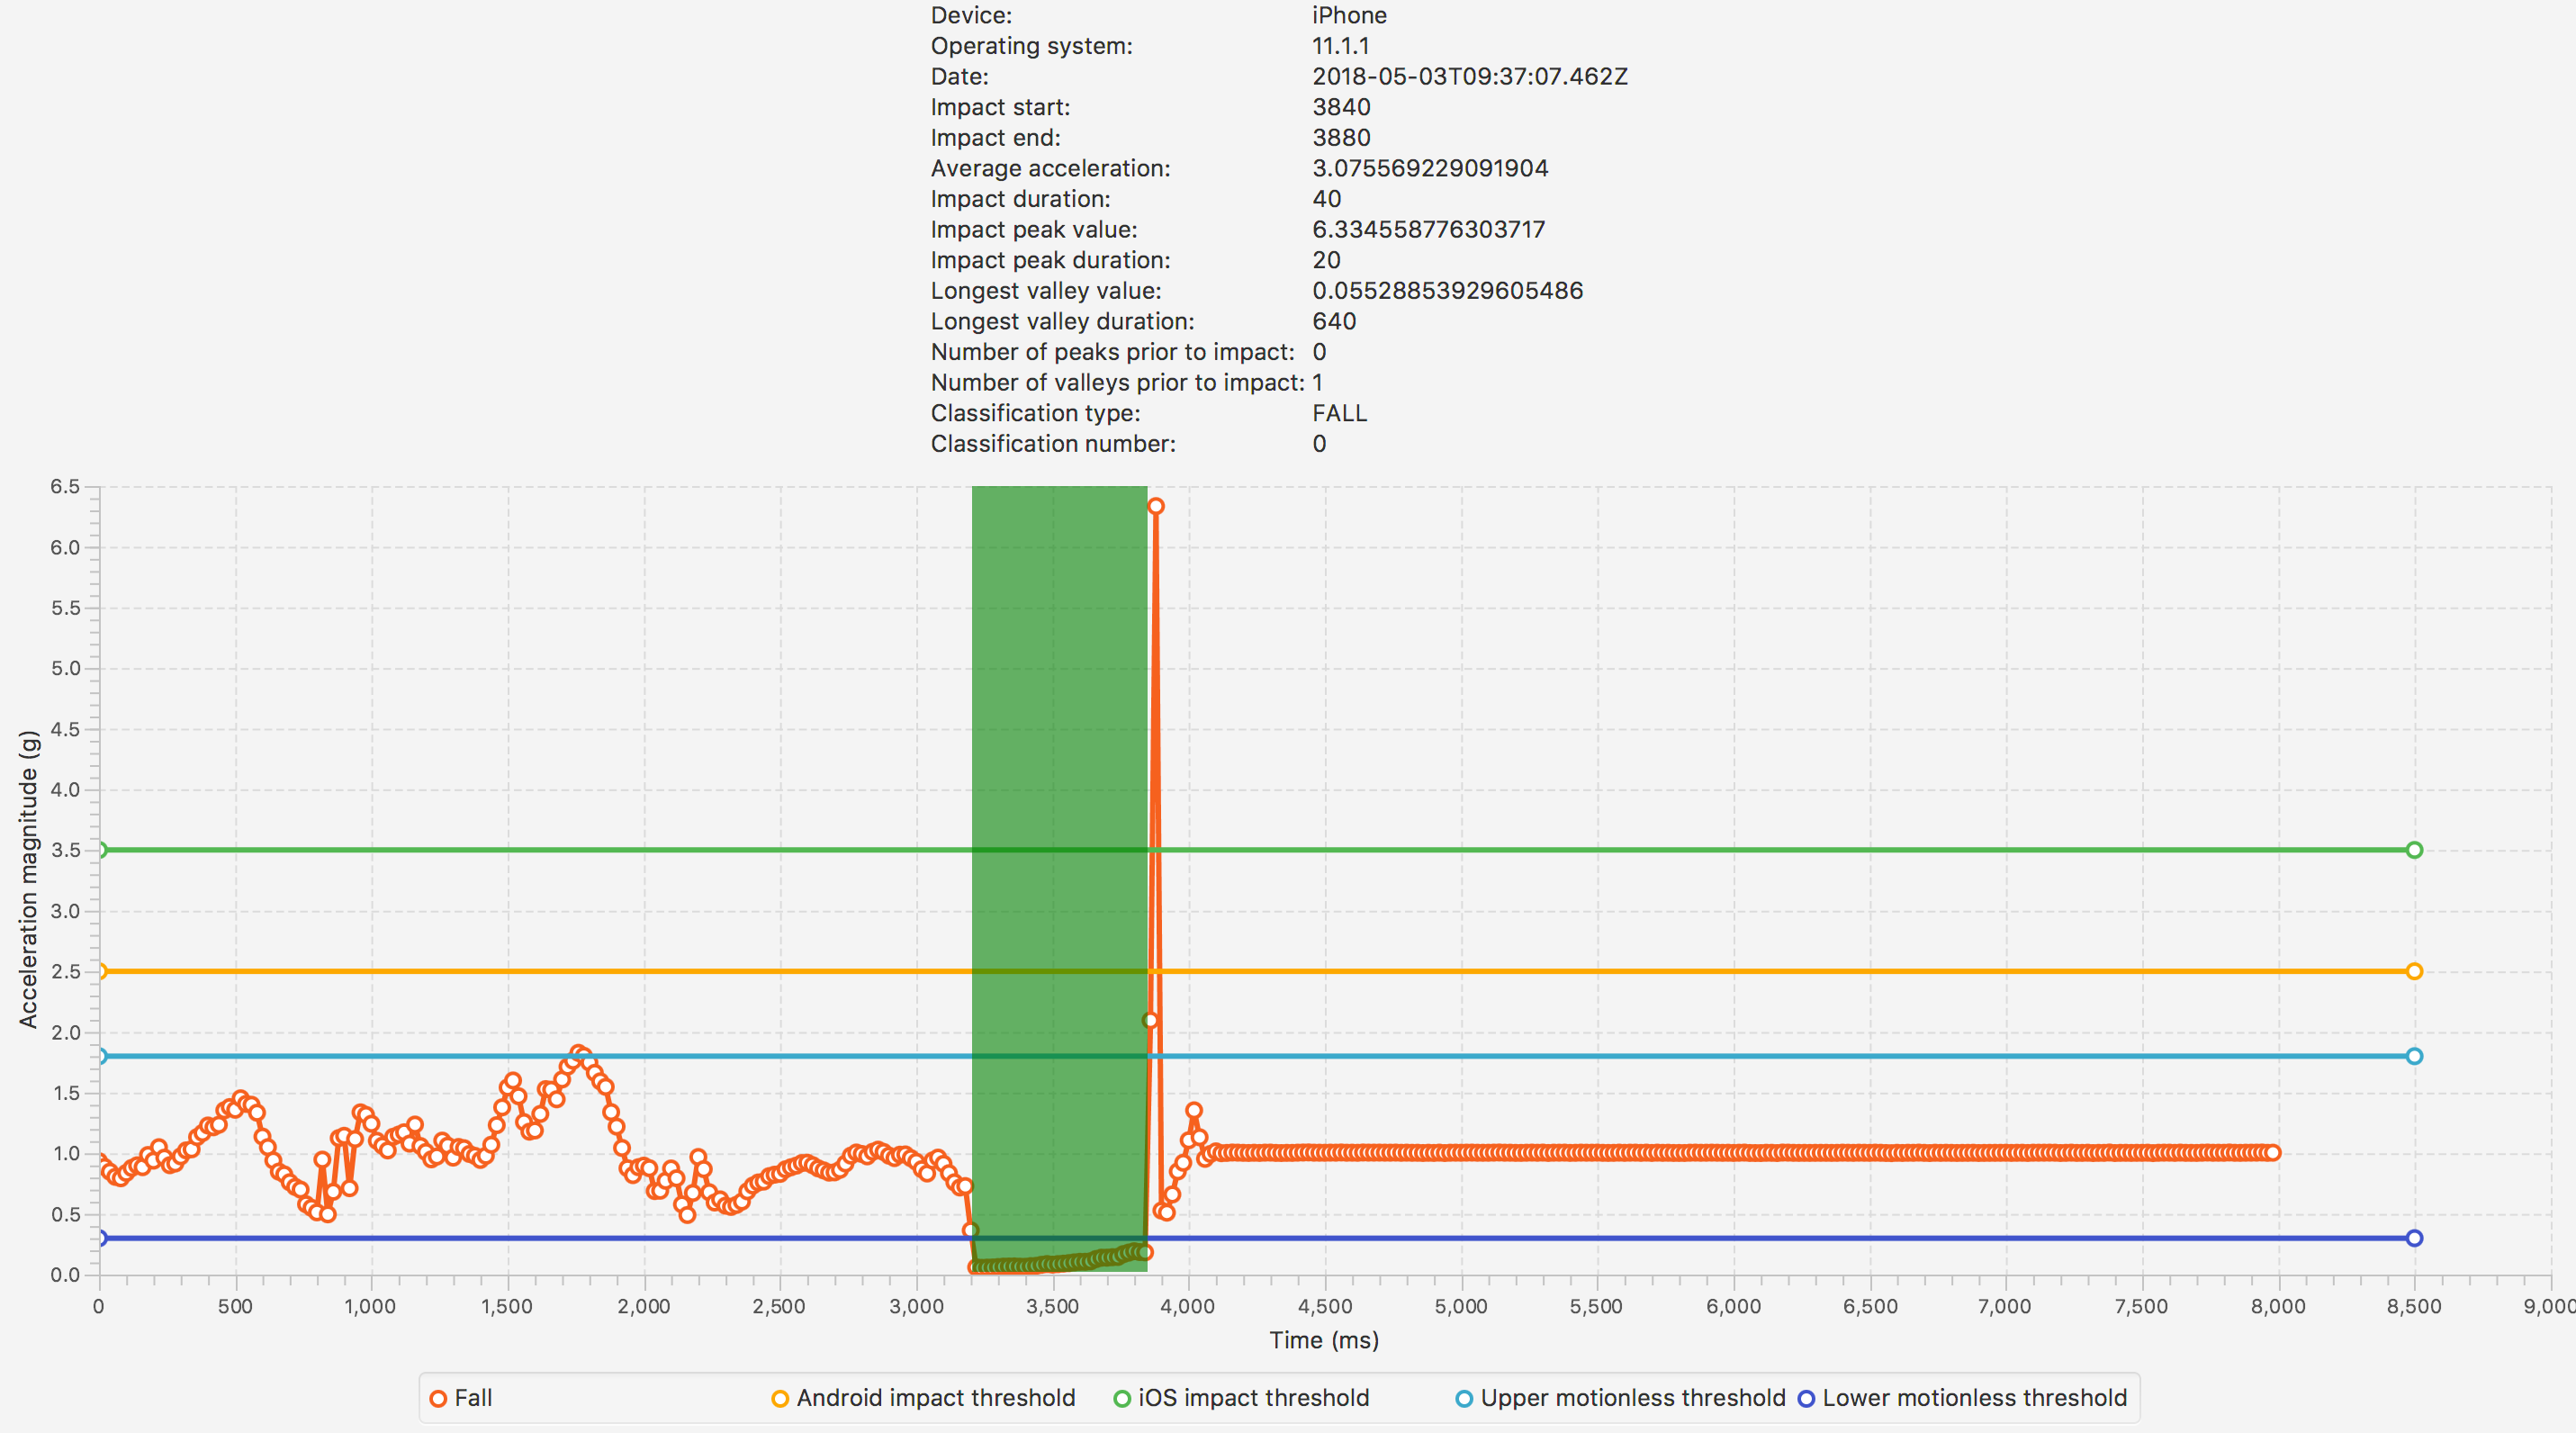
\includegraphics[width=14cm]{../img/fall-data-longest-valley-duration.png} }}%
		\caption{Visualization of longest valley duration. The longest valley duration is highlighted in green.}%
		\label{fig:fall-data-longest-valley-duration}%
	\end{figure}
	
	\subsubsection{Number of peaks prior to impact}
	
	The number of peaks prior to impact represents the number of continuous time intervals before the impact start, where each sample in the interval exceeds the impact threshold. Peaks prior to impact are highlighted in green in figure \ref{fig:fall-data-peaks-and-valleys}.
	
	\subsubsection{Number of valleys prior to impact}
	
	The number of valleys prior to impact is similar to the number of peaks prior to impact, but it counts the number of valleys instead of peaks. The valleys are defined as the continuous time intervals where each sample in the interval is below the lower motionless threshold. The valleys prior to impact are highlighted in red in figure \ref{fig:fall-data-peaks-and-valleys}.
	
	\begin{figure}[H]
		\centering
		\subfloat{{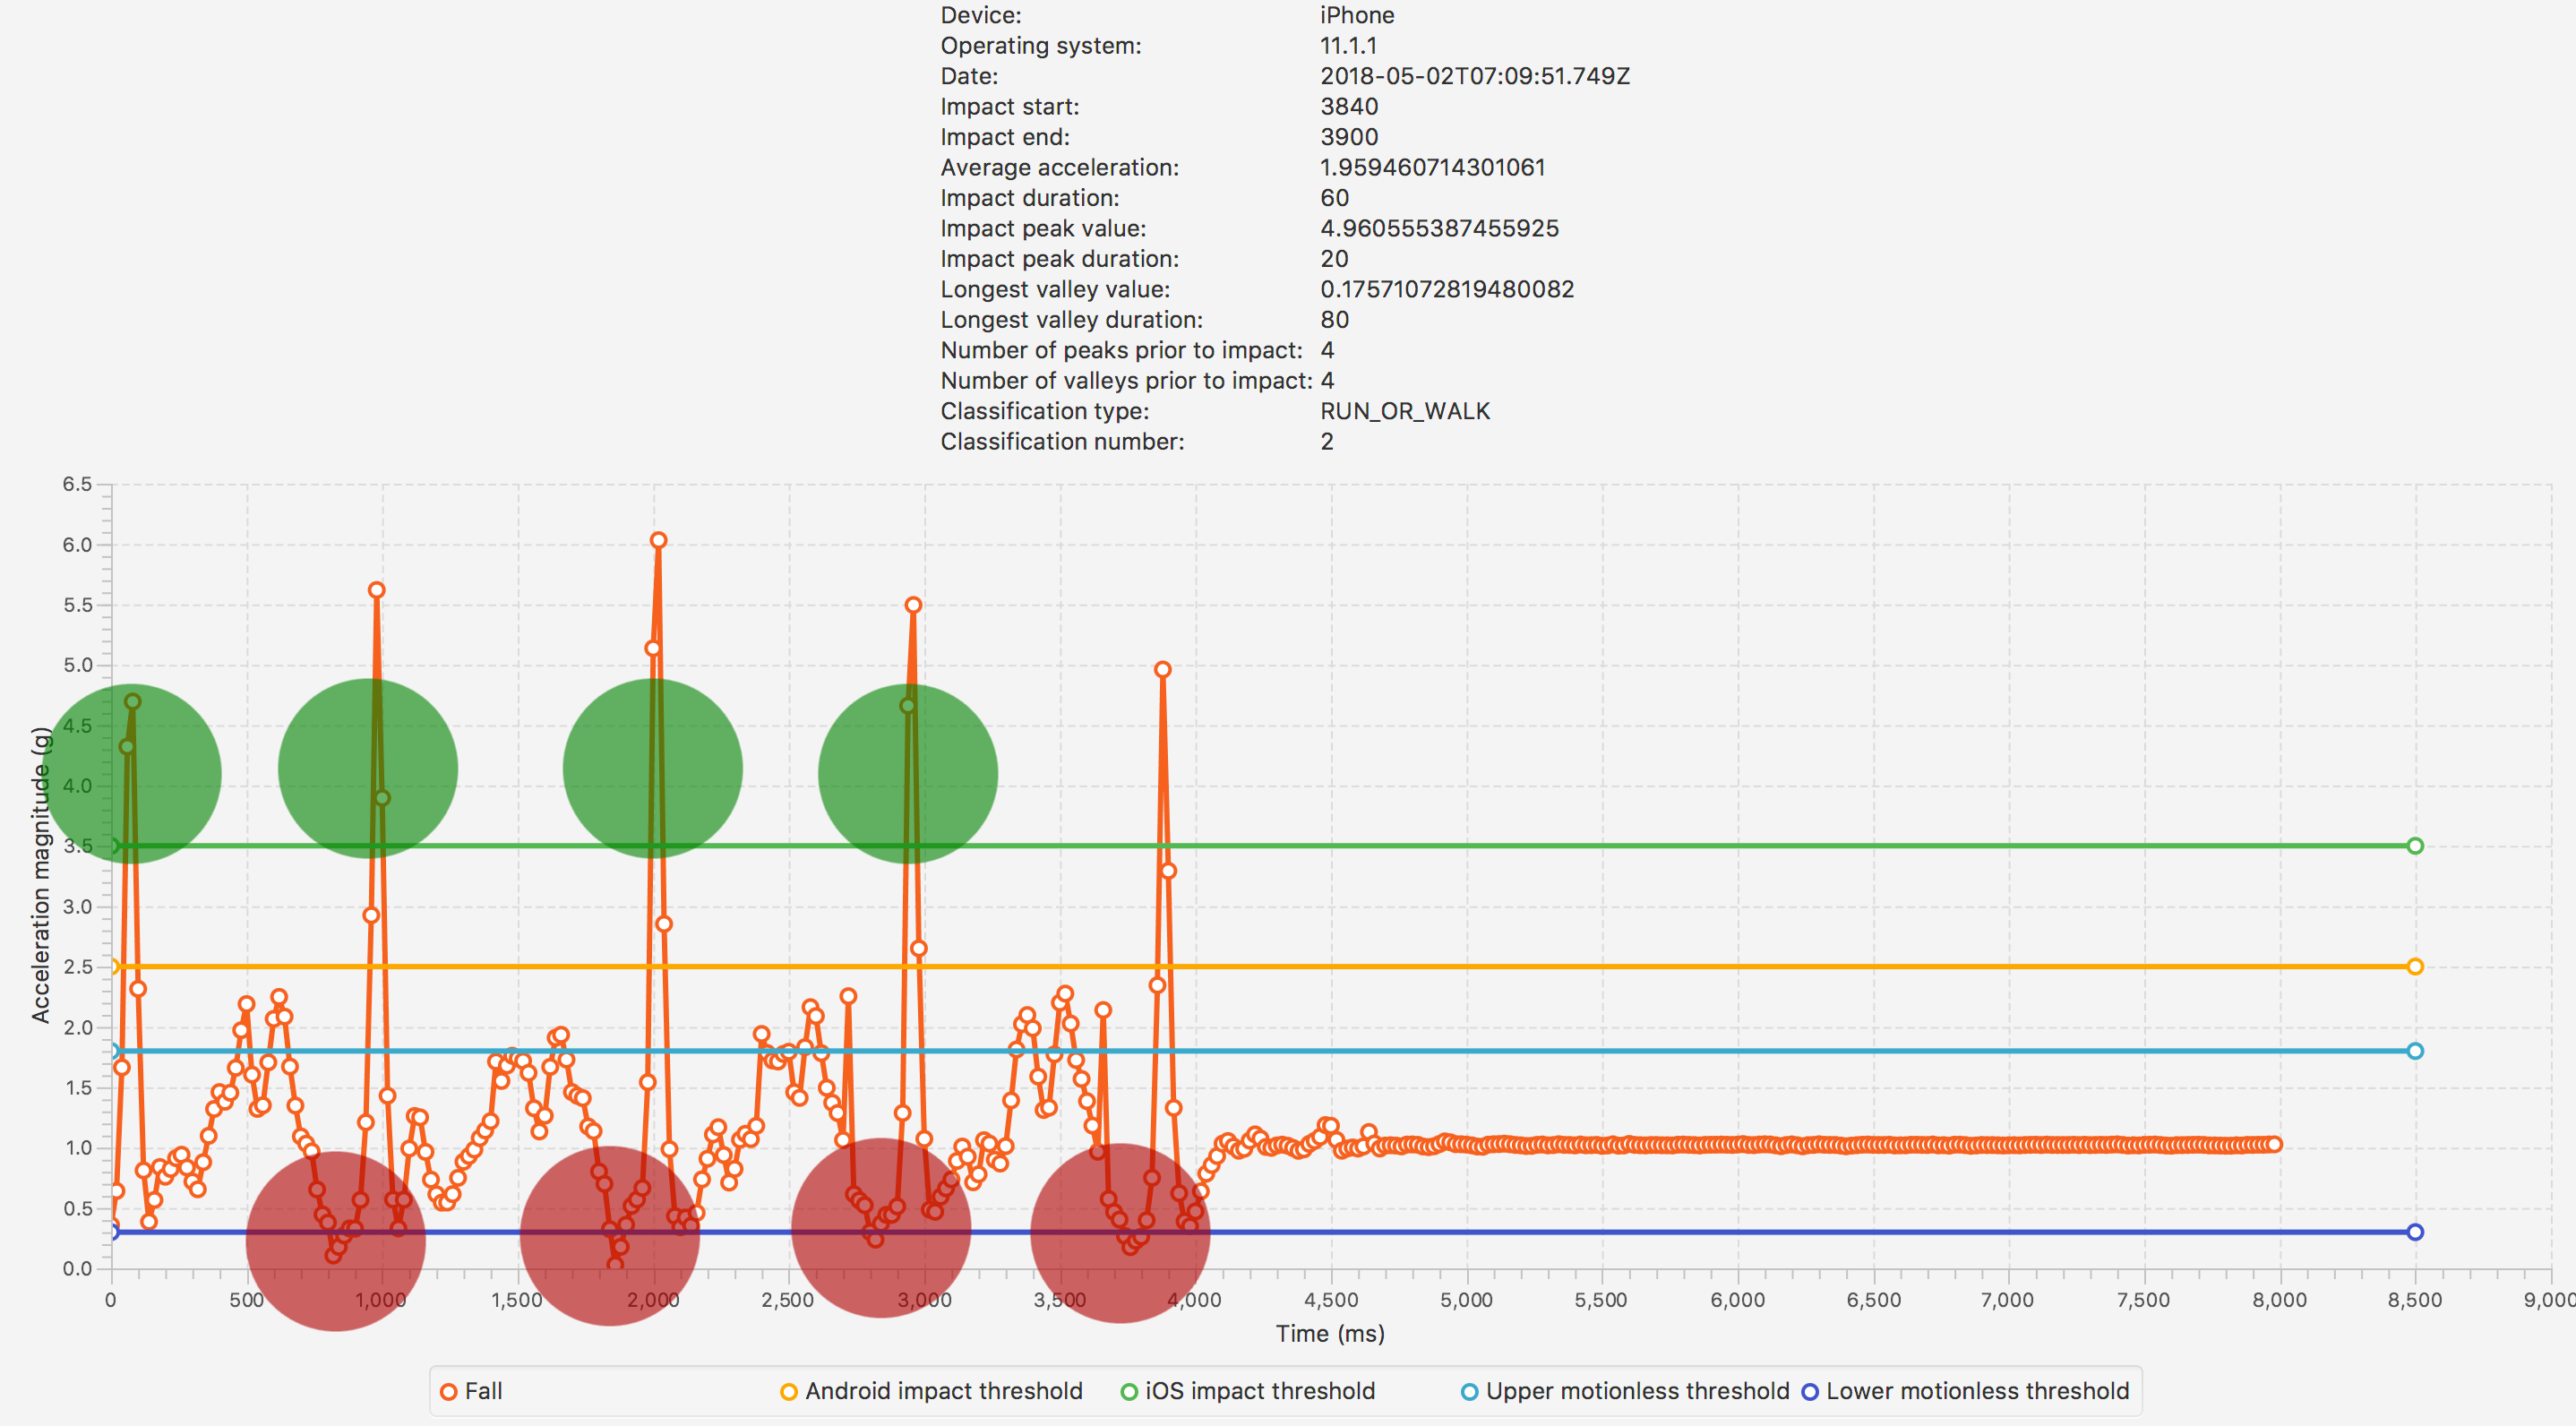
\includegraphics[width=14cm]{../img/fall-data-peaks-and-valleys.png} }}%
		\caption{Visualization of peaks and valleys prior to impact. The peaks are marked with green and the valleys are marked with red. In this example there are 4 peaks prior to impact, and 4 valleys prior to impact.}%
		\label{fig:fall-data-peaks-and-valleys}%
	\end{figure}
	
	\subsection{Implementing a neural network}
	The implementation of the neural network consists of three steps. The first step is related to data collection. The second step involves designing the network in terms on layers and neurons, \textit{this will from now on be referenced as the model}, as well as fitting and evaluating the model to make as accurate predictions as possible. The final step using the model in the application and evaluate its accurateness in real world scenarios. The full process from data collection to final model can be seen in figure \ref{fig:training-model}.
	
	\begin{figure}[H]
		\centering
		\subfloat{{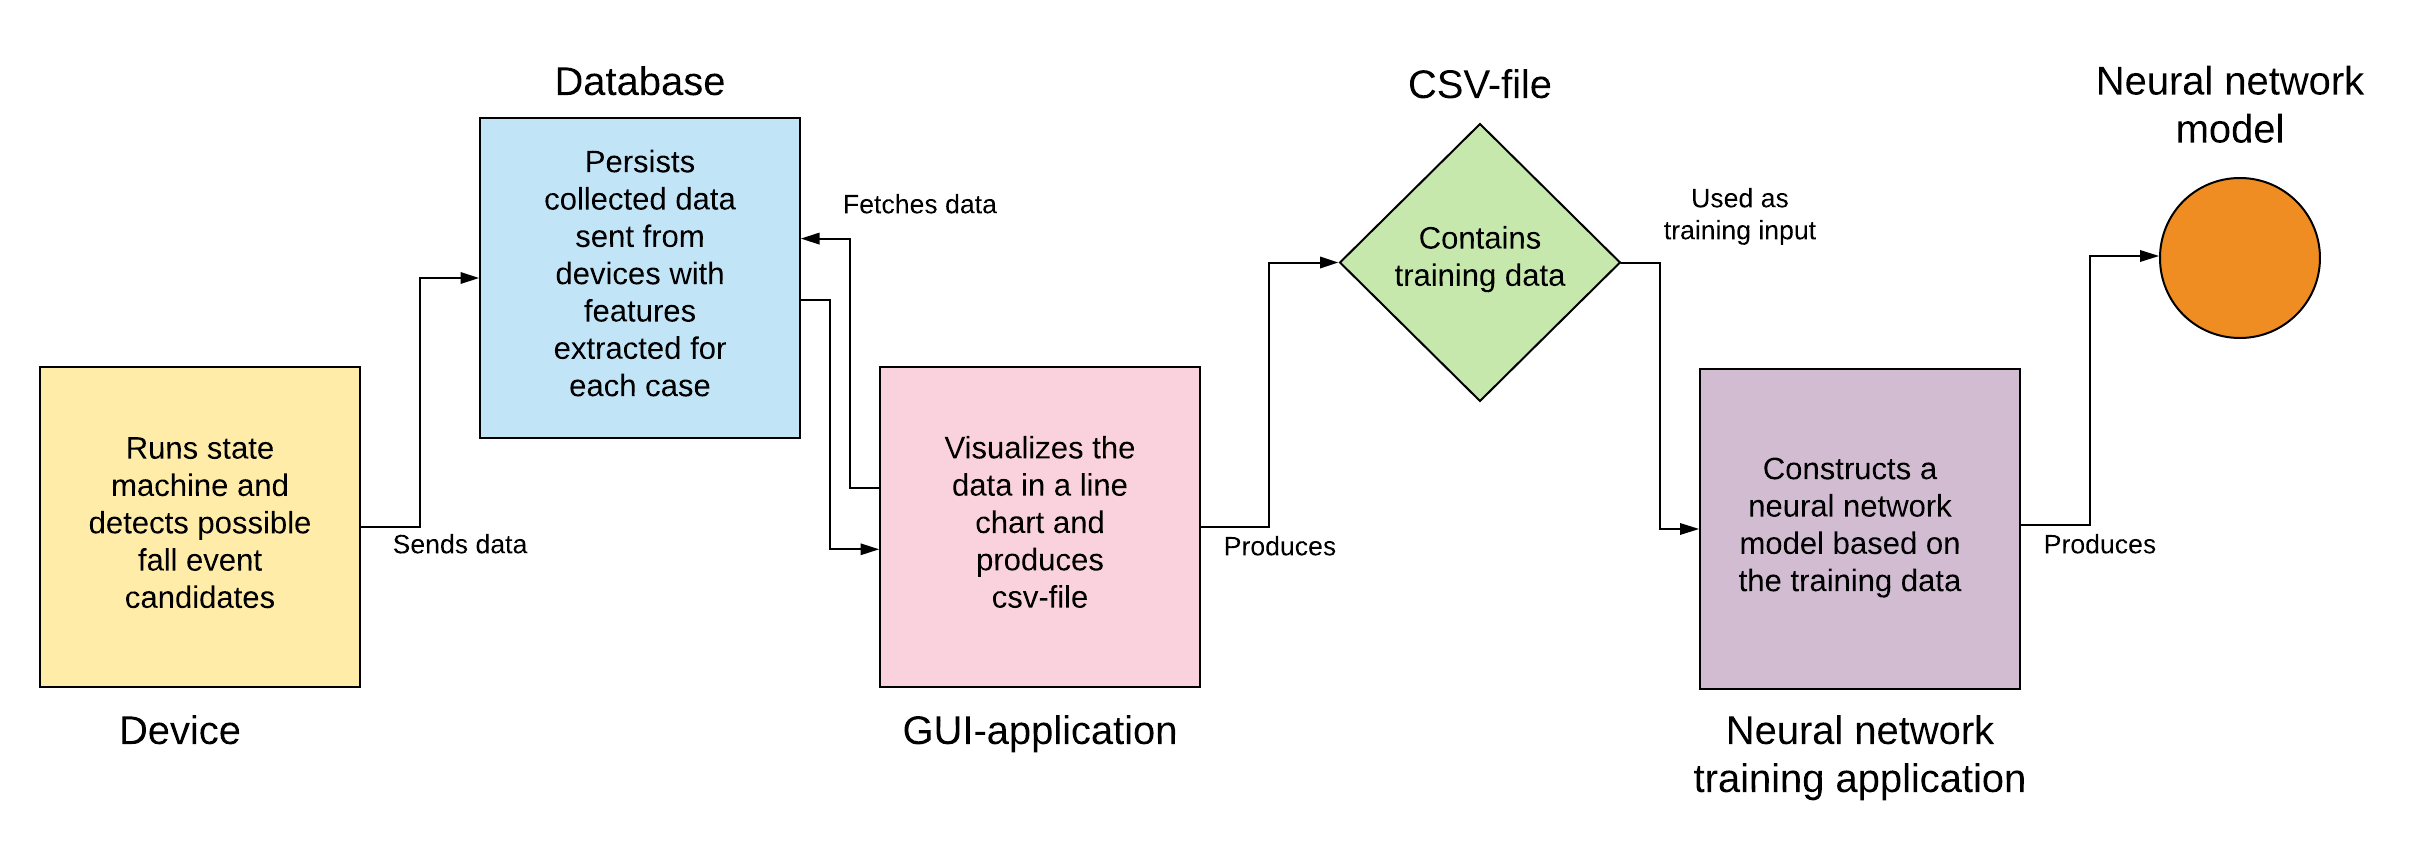
\includegraphics[width=15cm]{../img/training-model.png} }}%
		\caption{The process of collecting data and training the model}%
		\label{fig:training-model}%
	\end{figure}
	
	\subsubsection{Data collection}
	In order to collect motion data, we intercept every event that passed through our state-machine and following feature-extractor described in \textit{5.3} and \textit{5.4}. Thus, for all events that are recognized as a potential fall candidate, we have an object with its own set of the eight features described in \textit{5.4} as well as the original 400 sample long array of acceleration data collected from the accelerometer. The features are to be used when training the model and the array of data points is only used for visualization of the event on our graphical tool. Each event is labeled according to the class is belongs to \textit{fall, run/walk, jump}). The last step is to save each event to a database. 
	
	When collecting data for the \textit{run/walk} and \textit{jump} classes, we placed the device in the trouser pocket (\textit{a normal place to keep the device in everyday life}) and walked, ran and jumped respectively. Collecting data for the \textit{fall} class was done by letting the phone fall from different altitudes ranging from 1,5 m up to 3 m and landing on different natural surfaces. A series of events simulating falling while walking was also done by simply walking/running with the device and drop it to the ground mid walk.
	
	In total, 210 samples were collected, evenly distributed between the different classes and devices.
	
	\subsubsection{Designing a model}
	The neural network is built using \textit{Tensor Flow}, \textit{Keras} and the \textit{Python} programming language. After experimentation with the amount of hidden layers and neurons when training the model we arrived at the conclusion that a single hidden layer with seven neurons yielded the best possible accuracy given our data set. The activation function is set to \textit{sigmoid} for the hidden layer as well as the output layer. The result is a neural network with eight inputs, one for each feature, and three outputs, one for each class. 
	
	\begin{figure}[H]
		\centering
		\subfloat{{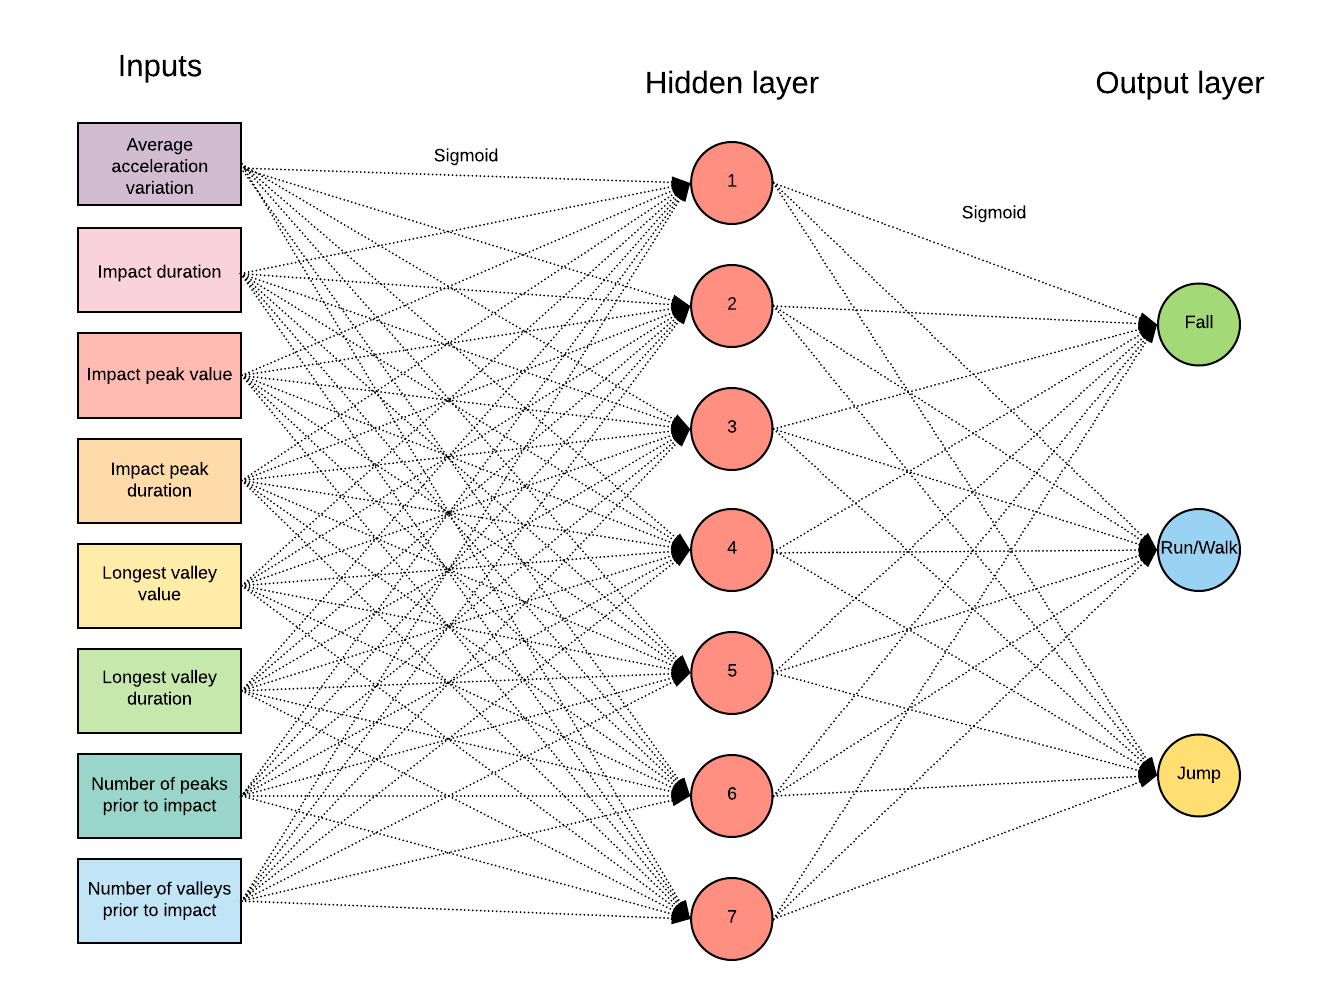
\includegraphics[width=15cm]{../img/neural-network-model.png} }}%
		\caption{The neural network}%
		\label{fig:neural-network}%
	\end{figure}
	
	\subsubsection{Training the model}
	When training the model, we downloaded all the data samples from the database and printed them to a CSV-file using our stand alone graphical utility tool. The dataset is then split up between training-set, and evaluation-set on a ratio of 9:1. The training set contains the labeled training data whereas the evaluation-set contains unlabeled data for measurement and cross-validation. The network training program uses the commonly used feed-forward <-> back-propagation method \cite{neural_networks} to fit the model. 
	
	
	\subsubsection{Using the model}
	The trained and evaluated neural network are finally converted into two separate file formats that can be used natively in iOS and Android applications. The generated files are simply included in the mobile application project after what they can be used to make predictions on future real life events. The input to the models are a vector of length eight, containing the values of the eight features for an event extracted by the feature-extractor. The output is a vector of length three, containing the independent probabilities of class adherence for the same event. 
	
	In the final product, where data collection functionality is removed, it is the values in the output vector that are used to finally decide if an event are to be classified as a fall accident or not. If the probability that the event belongs to the fall-class exceeds the other two, the application flags the event as a fall and presents the discard screen to the user, otherwise, the event will be automatically discarded by the application. 
	
	\newpage
	\subsection{Application user interface}
	
	Below is a rundown of the application user interface, only the most relevant view are shown.
	
	\begin{figure}[H]
		\begin{multicols}{2}
			\centering
			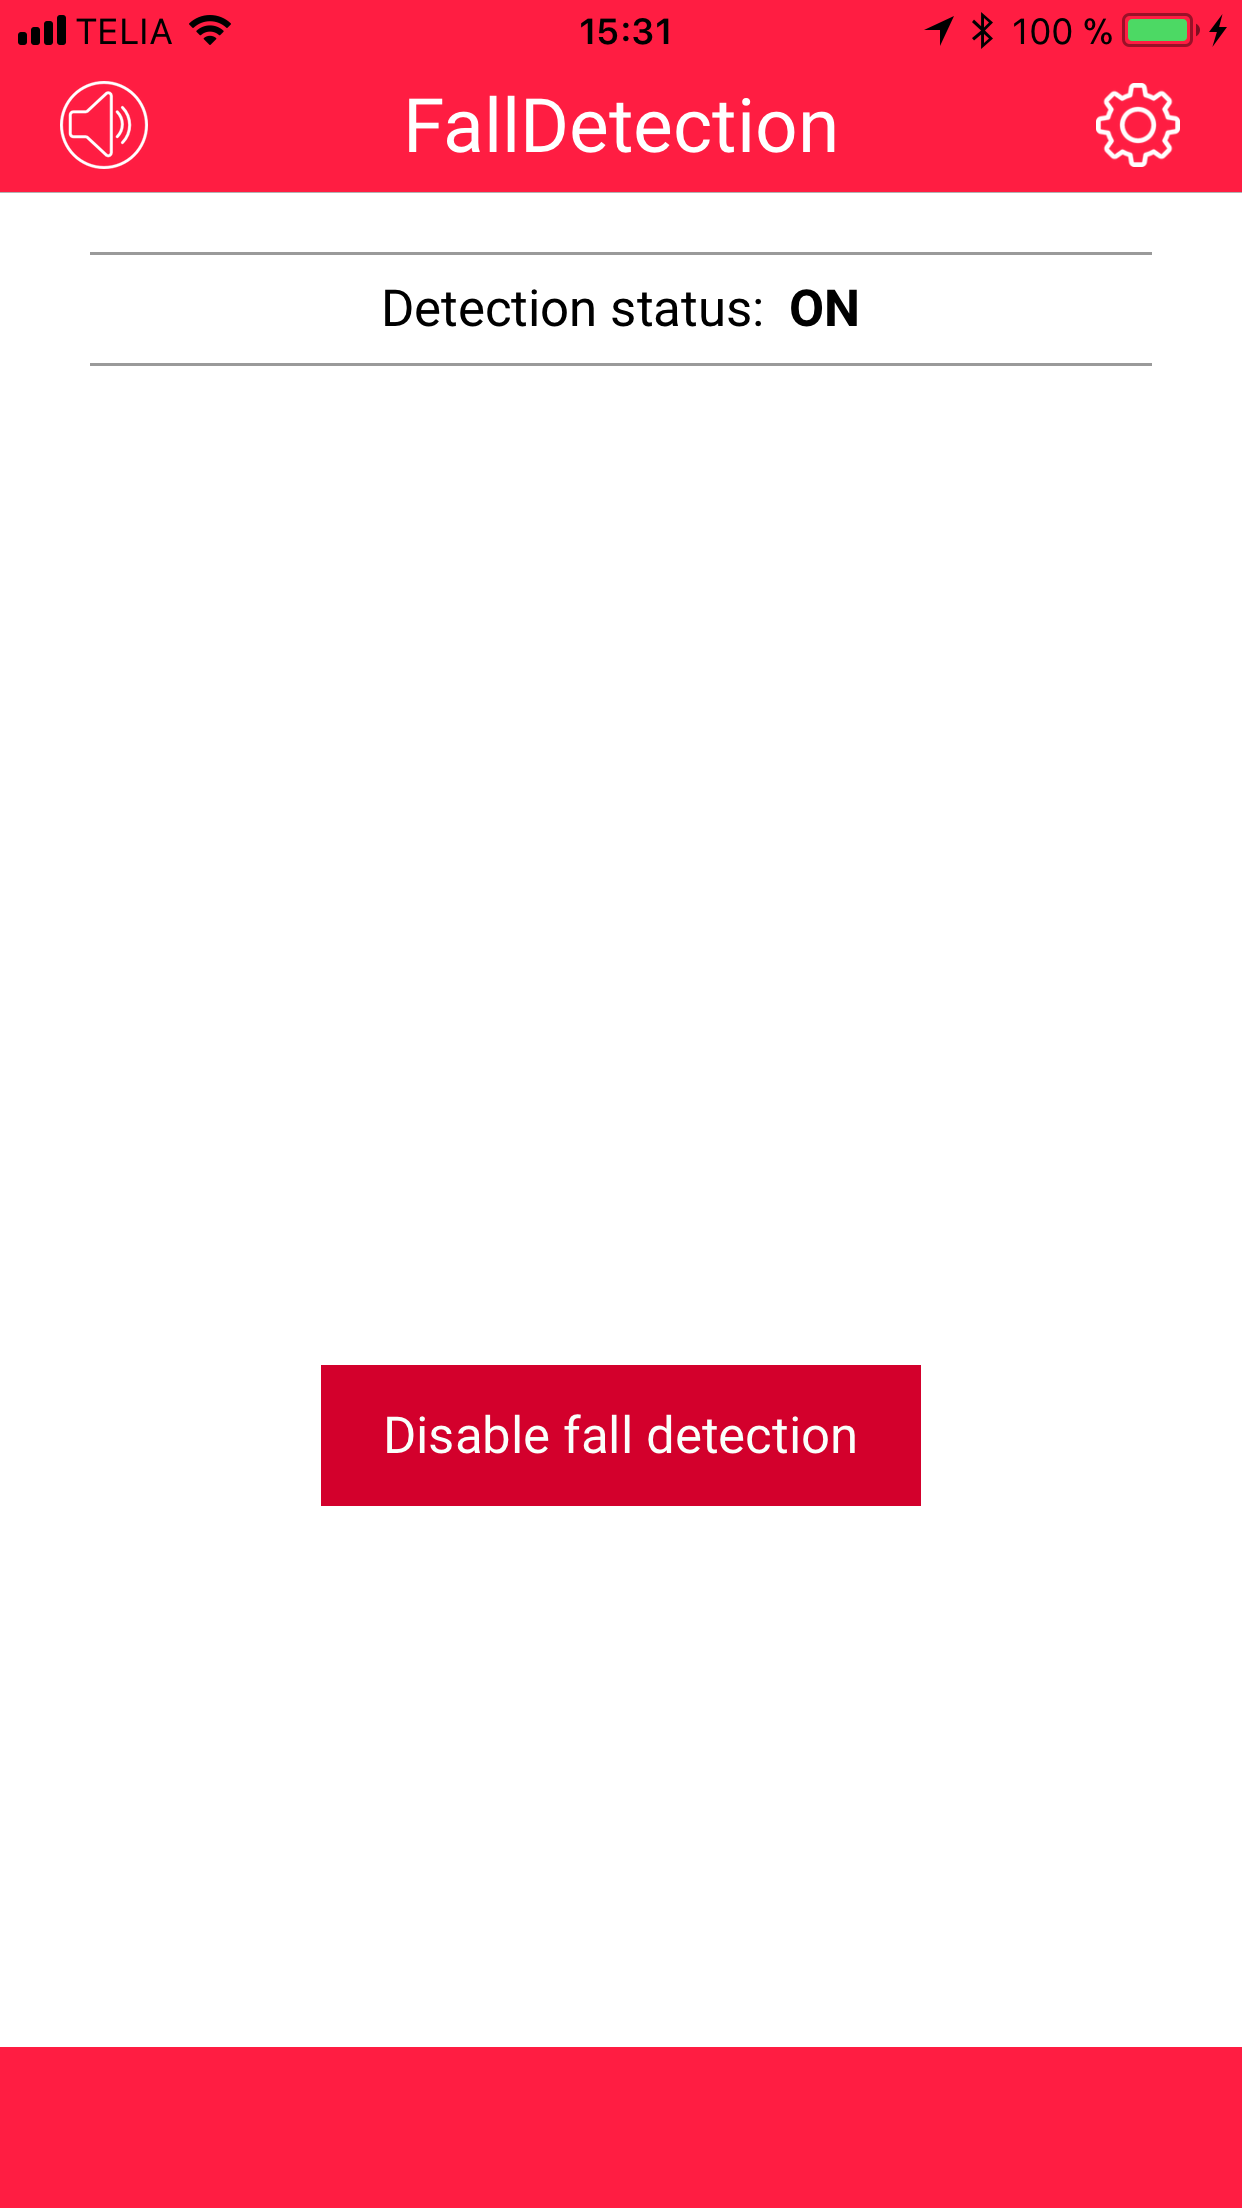
\includegraphics[width=6cm]{../img/screenshots/main-screen.jpg}\par 
			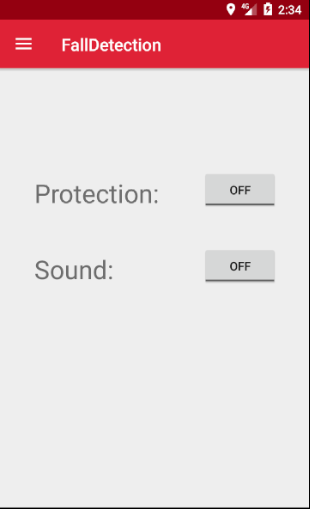
\includegraphics[width=6cm]{../img/screenshots/main-screen-android.png}\par 
		\end{multicols}
	\caption{The main interface of the application lets the user enable/disable fall detection as well as got to settings and toggle sonic alarm on/off. The iOS version is to the left, and Android to the right.}%
	\label{fig:main-screen}%
	\end{figure}
	
	\begin{figure}[H]
		\begin{multicols}{2}
			\centering
			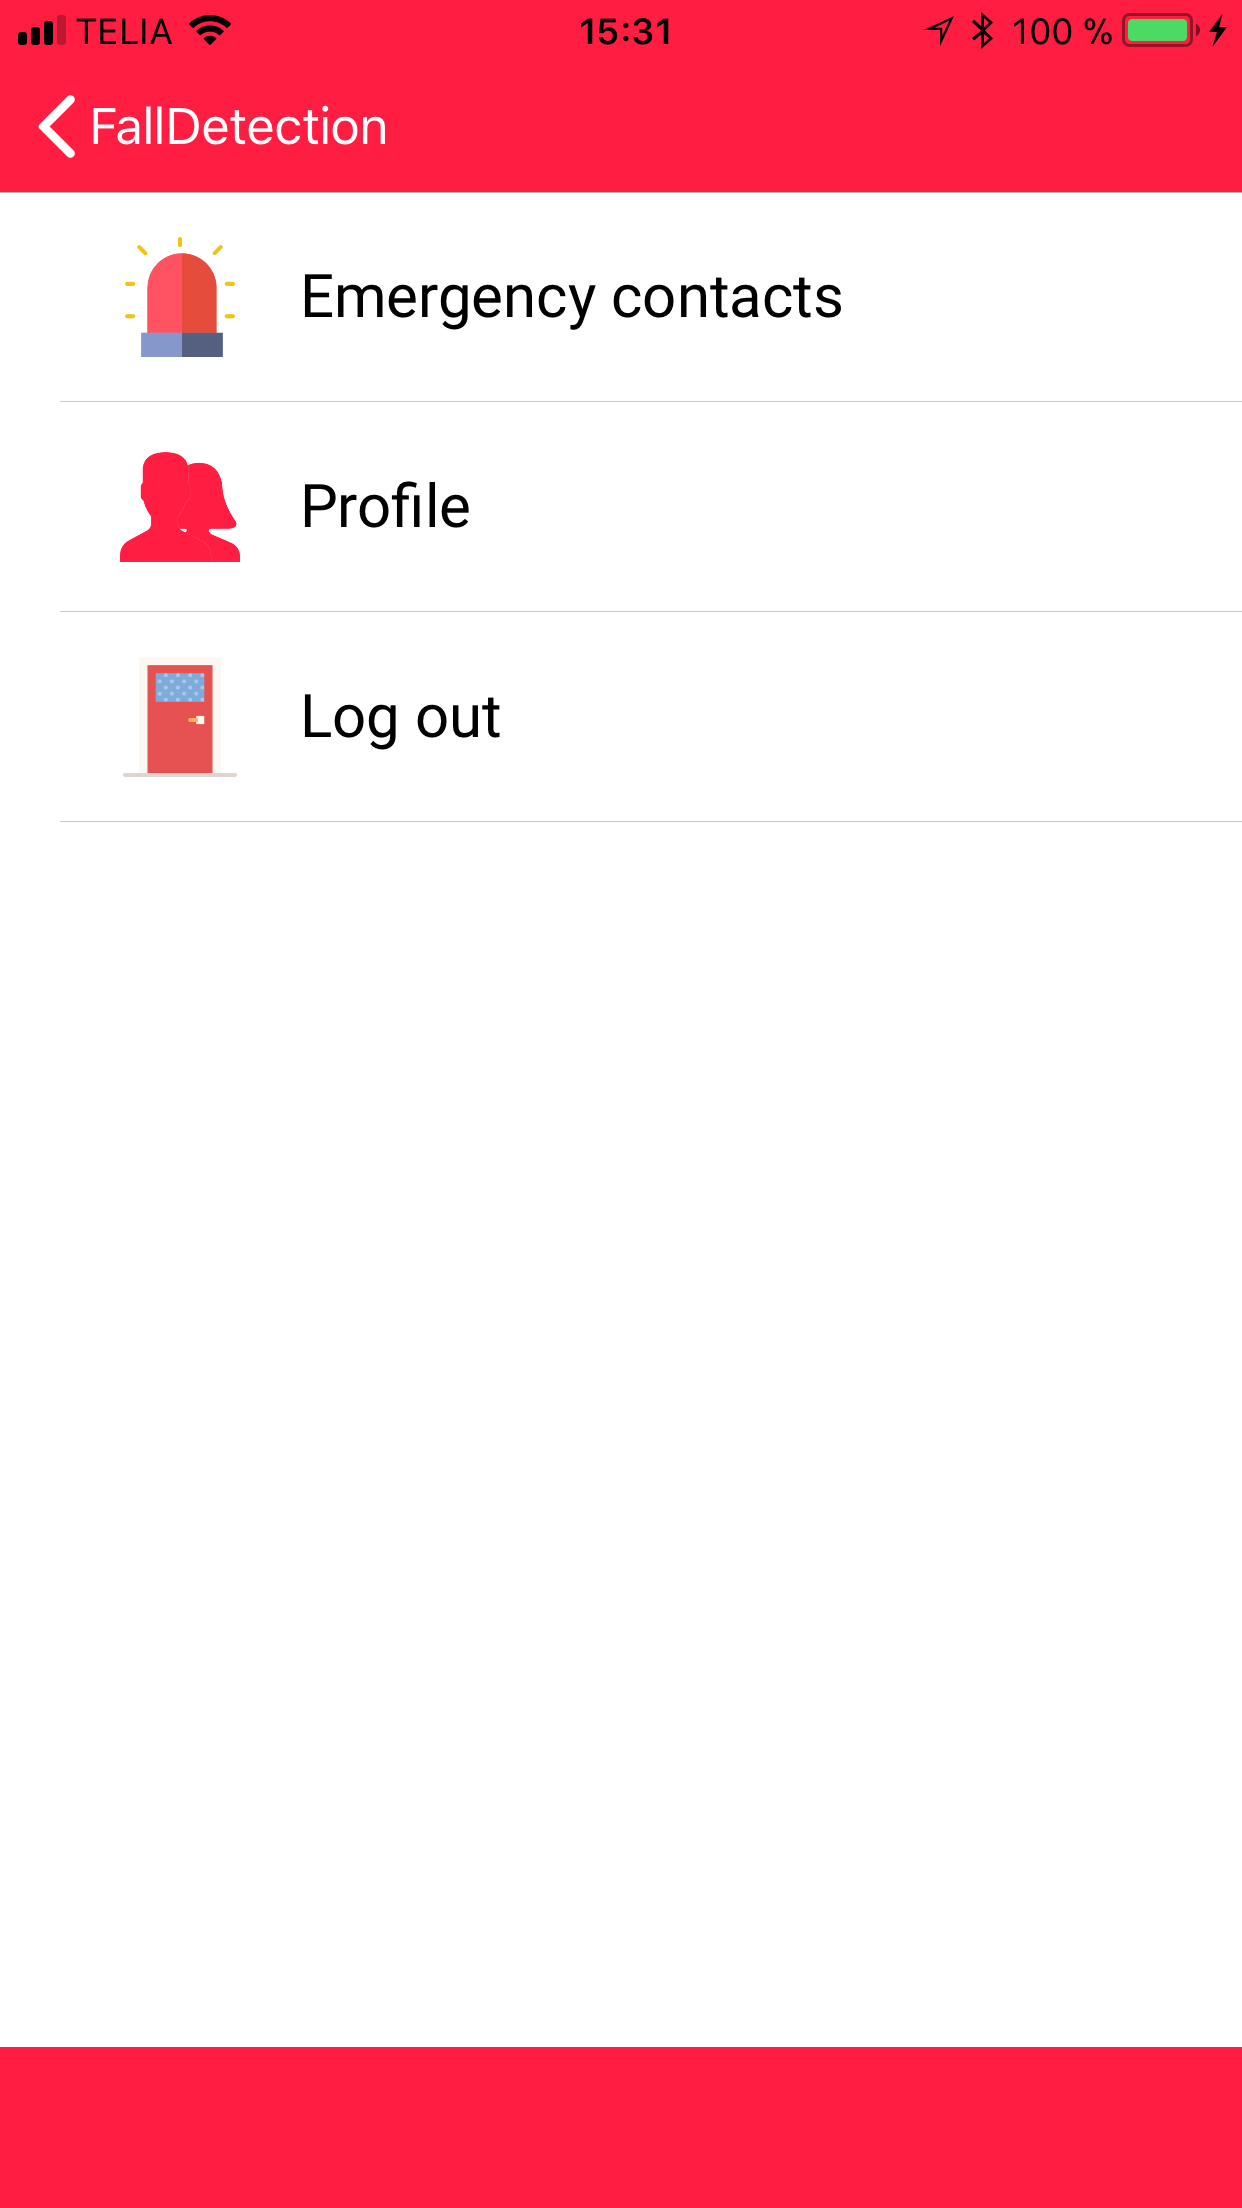
\includegraphics[width=6cm]{../img/screenshots/settings-screen.jpg}\par 
			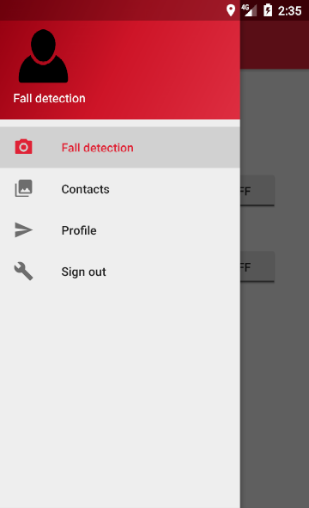
\includegraphics[width=6cm]{../img/screenshots/settings-screen-android.png}\par 
		\end{multicols}
		\caption{From the settings screen, the user can choose to view emergency contacts, his or hers profile and log out of the application. The iOS version is to the left, and Android to the right.}%
		\label{fig:settings-screen}%
		\end{figure}

		
		\begin{figure}[H]
			\begin{multicols}{2}
				\centering
				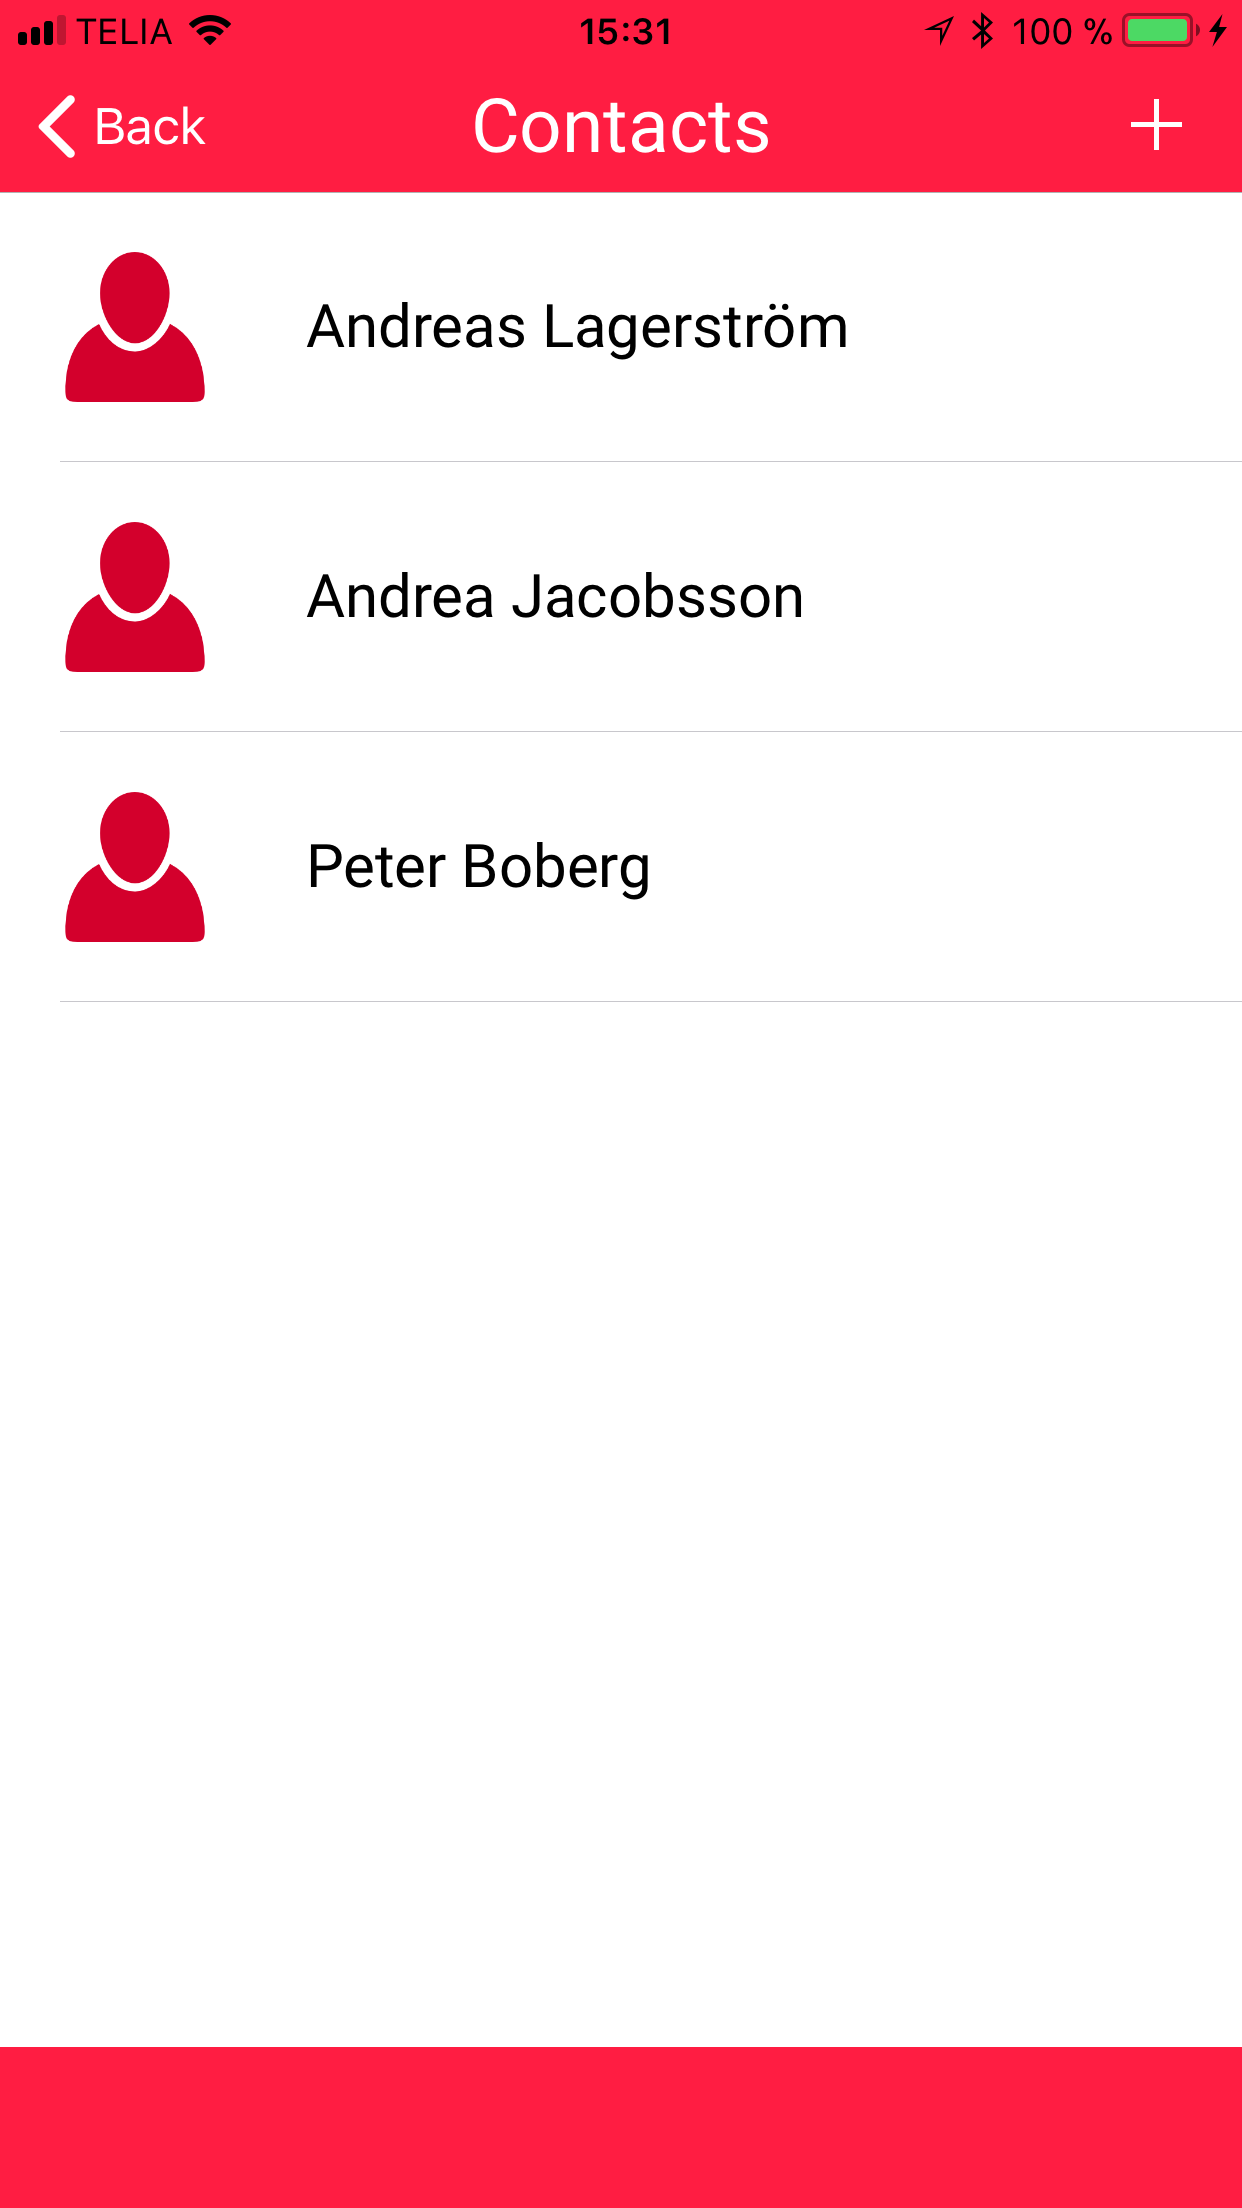
\includegraphics[width=6cm]{../img/screenshots/contacts-screen.jpg}\par 
				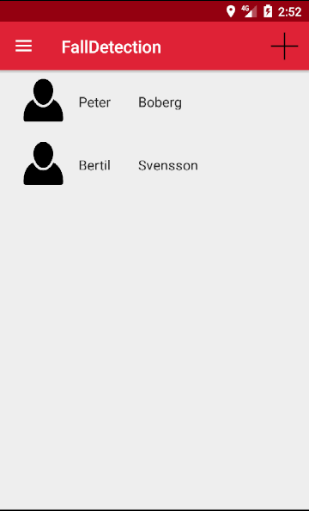
\includegraphics[width=6cm]{../img/screenshots/contacts-screen-android.png}\par 
			\end{multicols}
			\caption{The contacts screen displays all emergency contacts defined by the user. The user may also add a new contact by tapping the + sign. The iOS version is to the left, and Android to the right.}%
			\label{fig:contacts-screen}%
		\end{figure}
	
		\begin{figure}[H]
			\begin{multicols}{2}
				\centering
				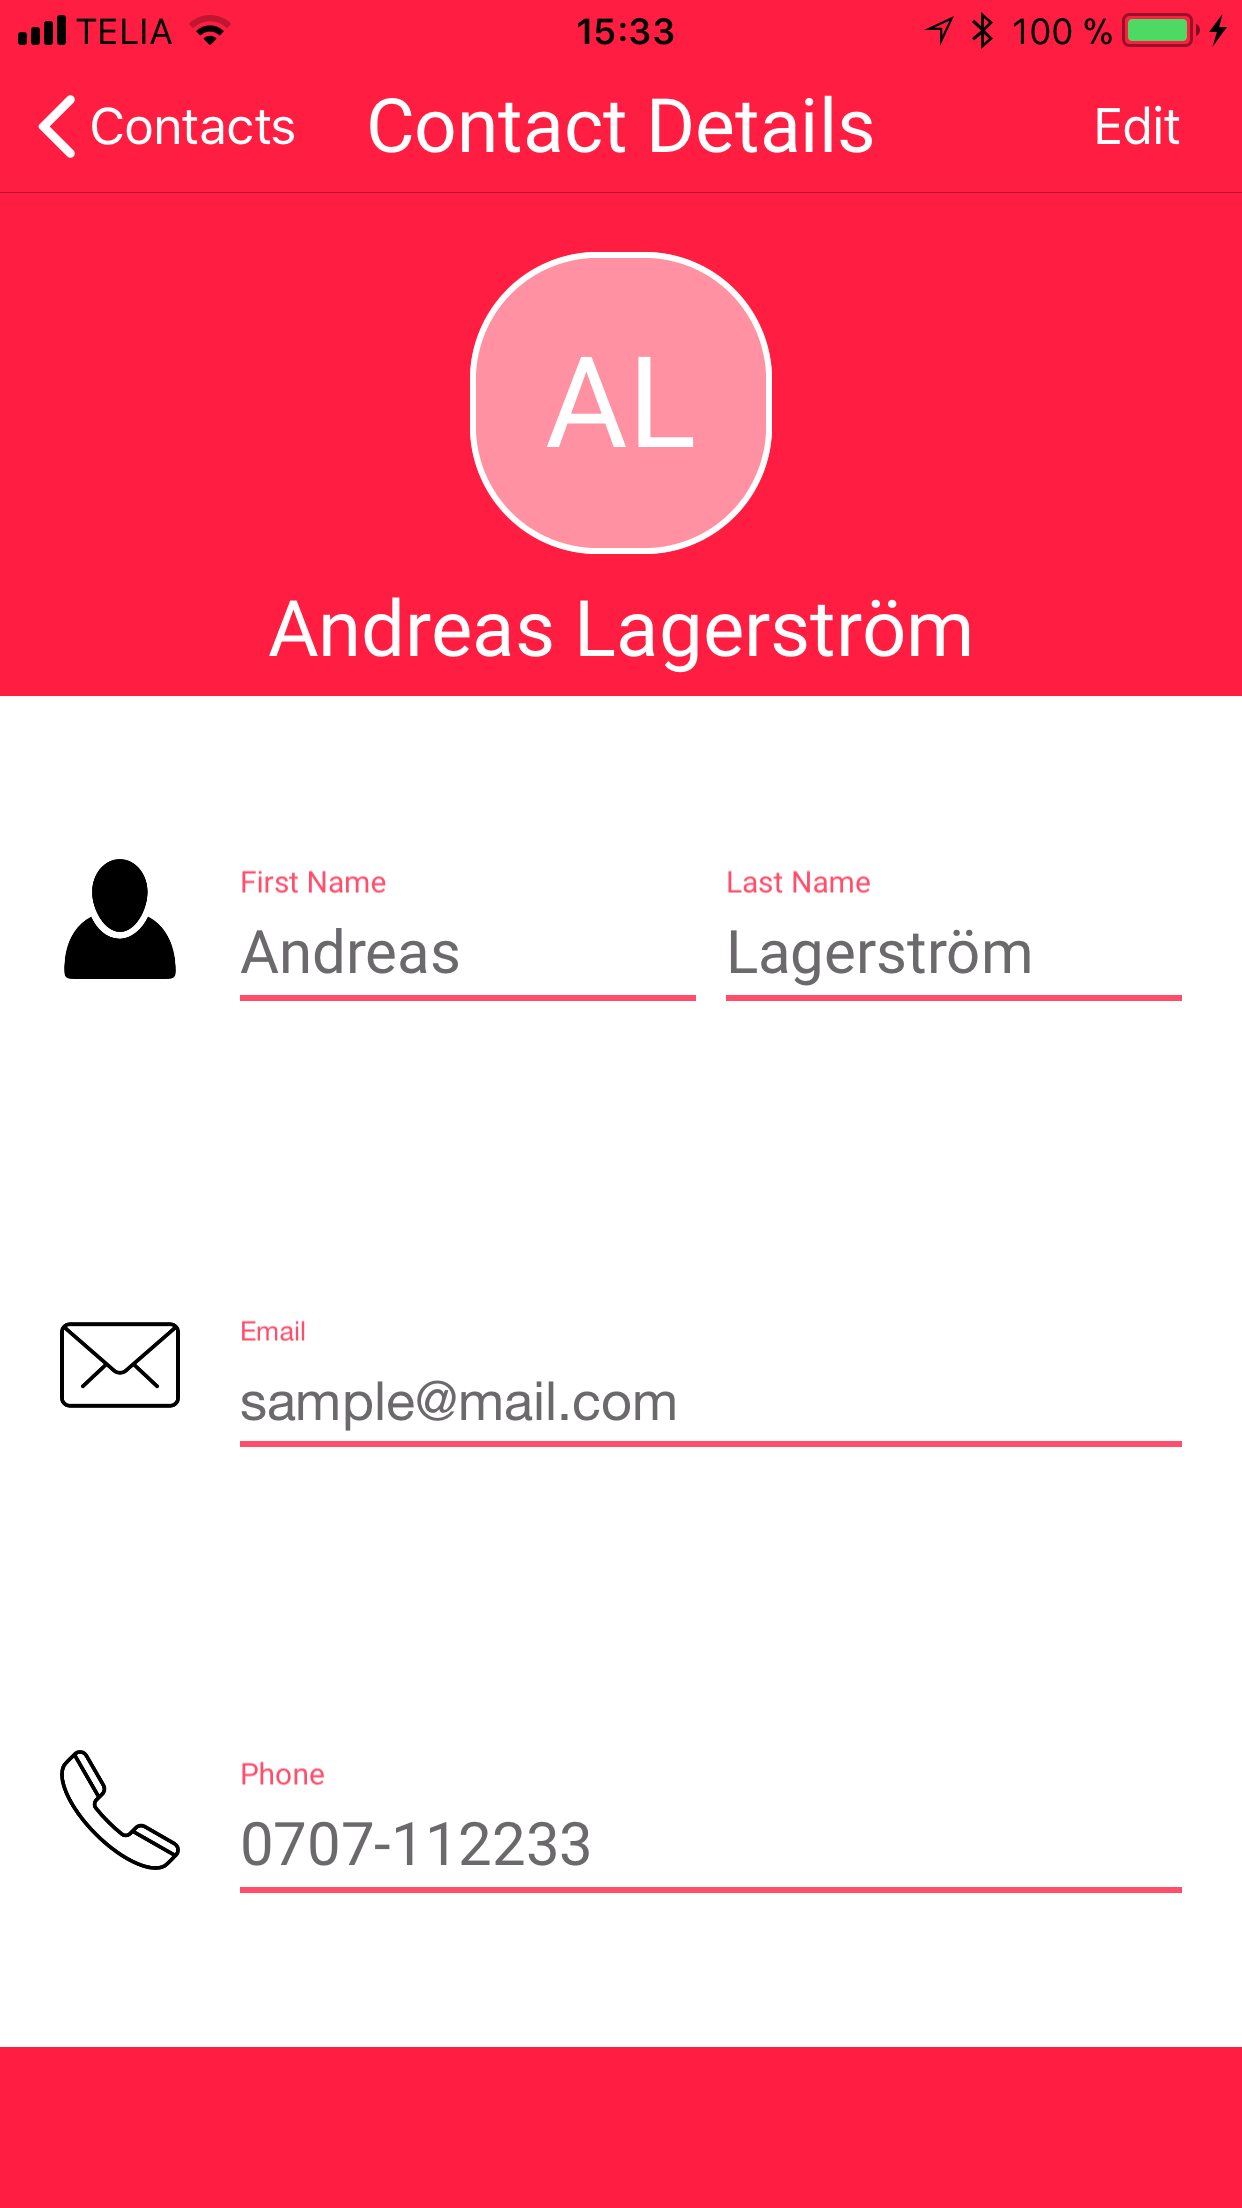
\includegraphics[width=6cm]{../img/screenshots/contacts-detail-screen.jpg}\par 
				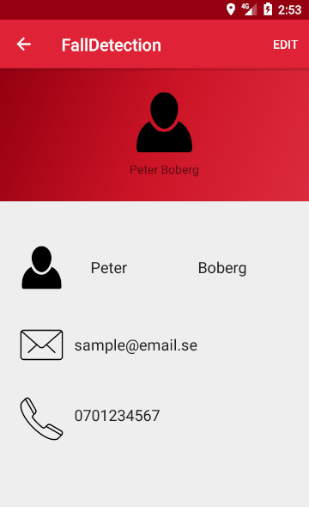
\includegraphics[width=6cm]{../img/screenshots/contacts-detail-screen-android.png}\par 
			\end{multicols}
			\caption{The contact detail view let the user view contact details as well as edit them by pressing the edit button. The iOS version is to the left, and Android to the right.}%
			\label{fig:contacts-detail-screen}%	
		\end{figure}

		\begin{figure}[H]
			\begin{multicols}{2}
				\centering
				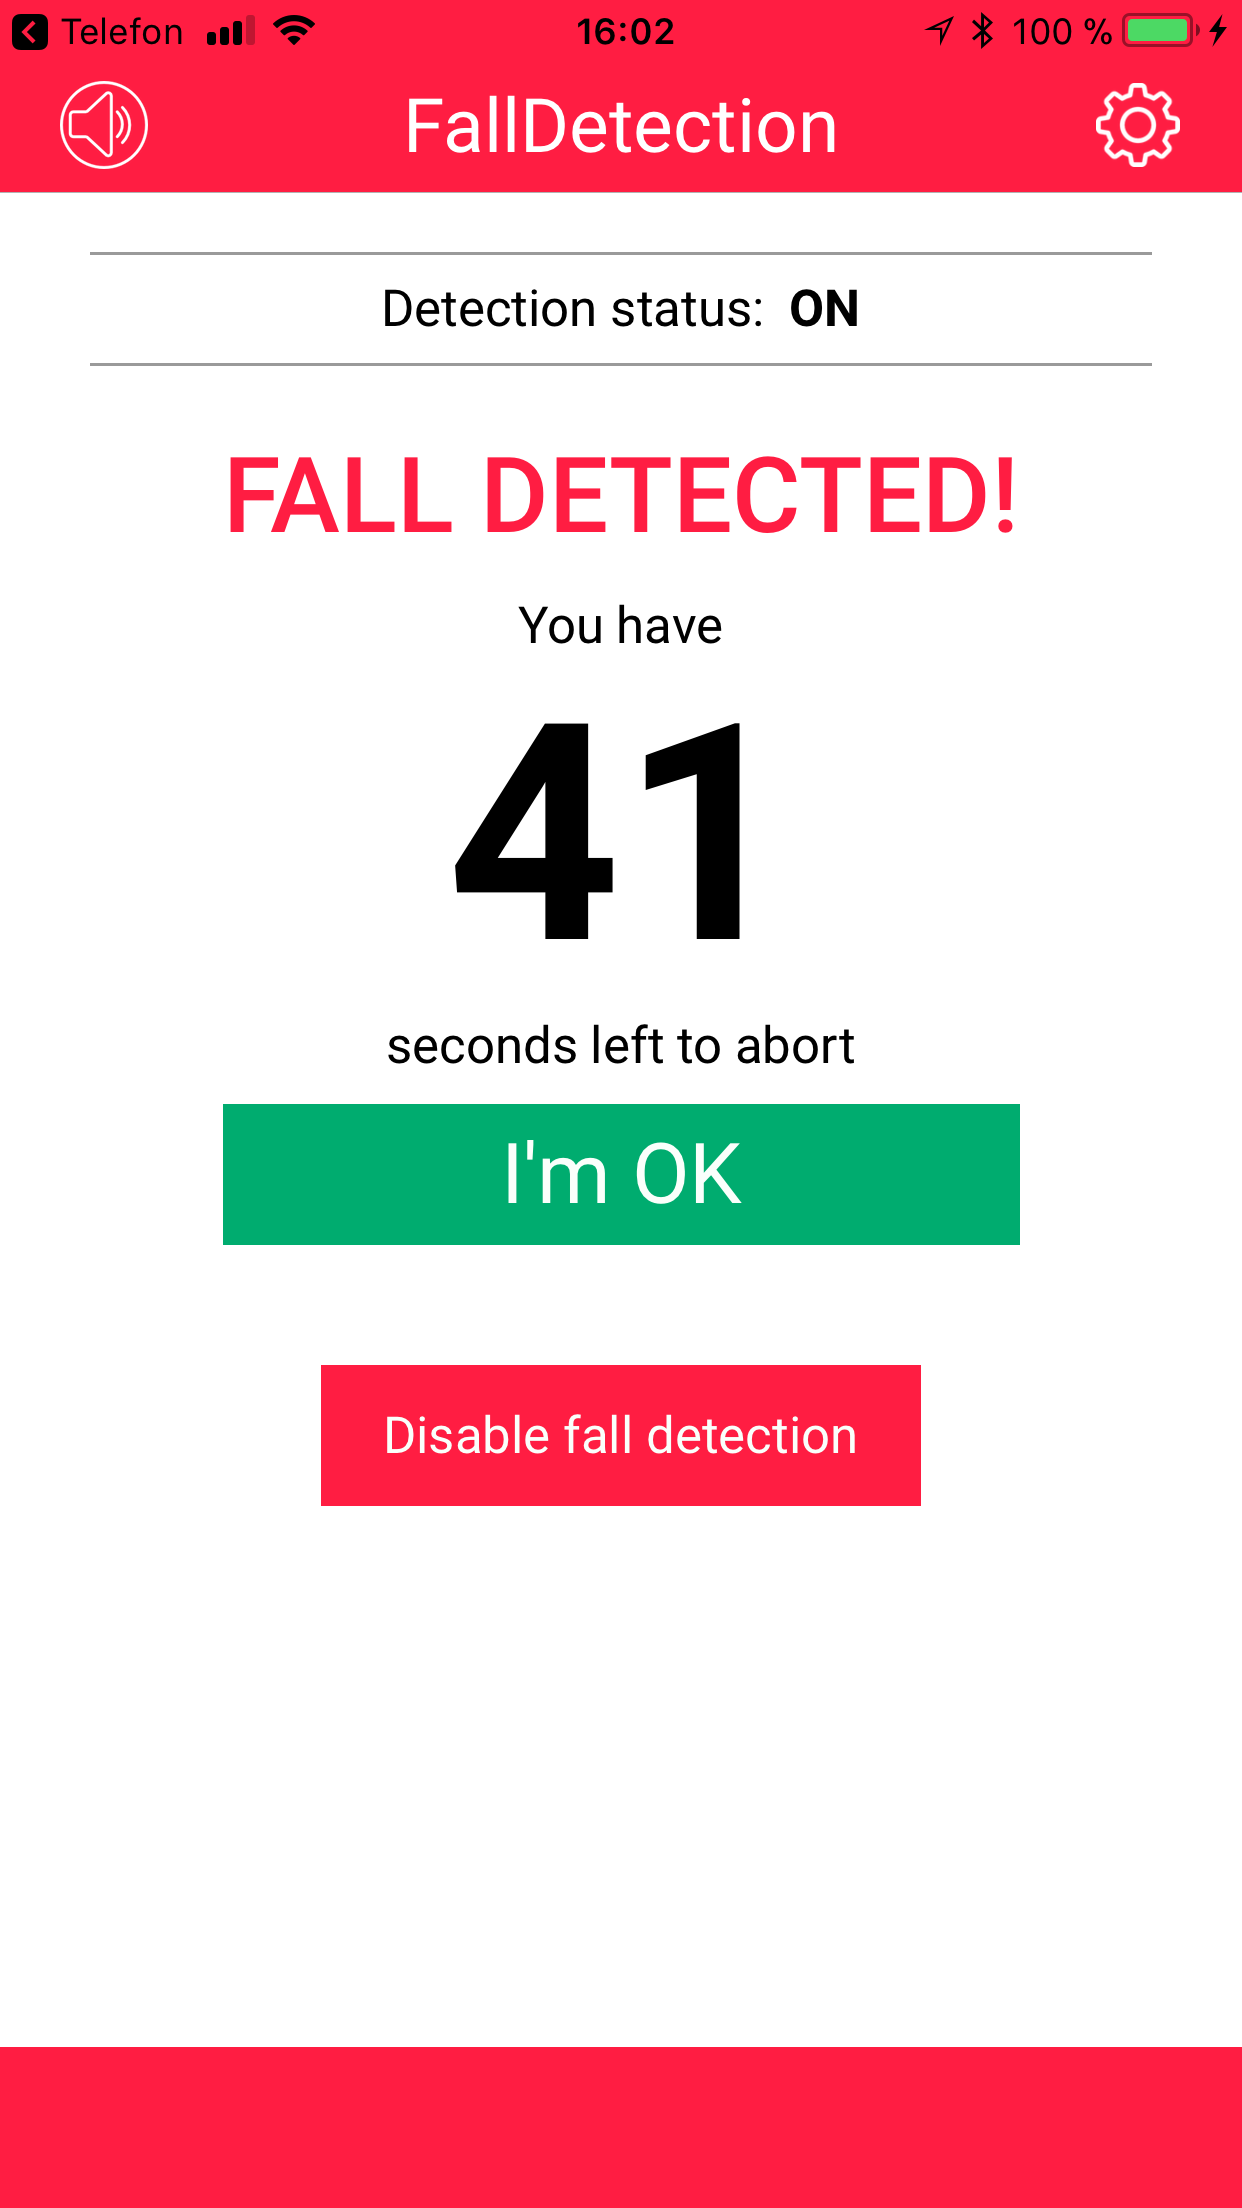
\includegraphics[width=6cm]{../img/screenshots/alarm-screen.jpg}\par 
				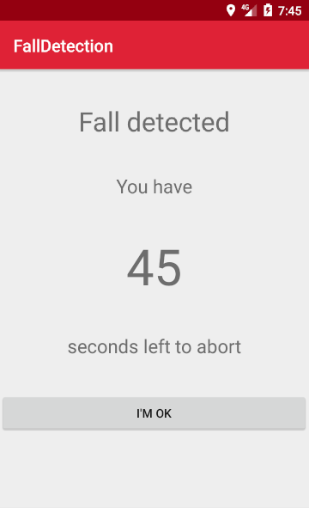
\includegraphics[width=6cm]{../img/screenshots/alarm-screen-android.png}\par 
			\end{multicols}
			\caption{The alarm screen is shown when the app detects a fall, the user now has 45 seconds to discard the event by pressing "I'm OK", or an email containing information and coordinates will be sent to the users emergency contacts when the timer fires. The iOS version is to the left, and Android to the right.}%
			\label{fig:alarm-screen}%
		\end{figure}
	
	\newpage
	\section{Fall Detection Application: Evaluation}
	
	
	\newpage
	\section{Discussion \& Conclusions}
	
	In this chapter, the methods used in the study and their implications are analysed, the research questions are answered followed by a discussion of sustainability and ethical considerations. Lastly, the research project is summarized and suggestions for future research is presented.
	
	\subsection{Methods \& Implications}
	
	This section analyses the methods used and the validity and reliability of this study.
	
	\subsubsection{Literature study}
	
	Since very similar studies had already been conducted before we started this research project, it was necessary to perform a literature study before starting the development process. Without this literature study we would not have known how previous researchers had reasoned and it would have been likely that we had repeated old mistakes and ended up with a lesser application.
	
	\subsubsection{Case study: Development}
	
	The case study consisting of developing an application gave us the opportunity to test different approaches and ideas to see if the algorithm could be improved. Developing an application was necessary since we did not have access to the source code of any existing application.
	
	\subsubsection{Evaluation}
	
	\subsubsection{Validity \& Reliability}
	
	This section discusses the validity and reliability of the study.
	
	\parag{Validity}
	The term \textit{validity} is referring to whether or not the research methods are measuring what the study is trying to answer. With respect to the first research question, RQ1, regarding how a fall detection application can be created, it should be clear that the case study is addressing this question since it is exactly what is done in the case study. Regarding the second question, RQ2, it is not as obvious. To answer how this kind of application affects battery life, you could argue that it would be better to measure the battery consumption of many different fall detection applications and draw conclusions based on that. This would however give pure statistical knowledge saying that application A consumes X amount of battery per hour and application B consumes Y. Without insight into how these applications function internally this kind of information says nothing -- it would not be possible to say why application A consumes more power than B, or the other way around. To perform such a comparison and to say why one application consumes more power than the other, it would be necessary to have the source code to the different applications, something that we did not have. Therefore this study can only say that if an application is developed the way that we did, you can expect that the battery consumption will be similar to the consumption in our measurements.
	
	\parag{Reliability}
	\textit{Reliability} refers to how replicable or repeatable the research project is. Another research project that asks the same questions and and uses the same methods should ideally come to the same conclusions. Our first method was to perform a literature study with the intention to find a good algorithm that were to be used as a starting point for the case study. It should be noted that another researcher, with different background and experiences may have found another algorithm as a better starting point and ended up with an application that implements fall detection entirely different, and thus could have ended up with different conclusions. However, if another researcher would use the same starting point as we did, and make the same decisions along the way, s/he should end up with the same result, and therefore the work is repeatable.
	
	\subsection{Revisiting research questions}
	
	This section answers the research questions.
	
	\textbf{RQ1} \textit{How can a mobile application, that detects falling accidents using modern smart phones, be created?}
	
	Based on the case study, we saw that a mobile application can be created so that it successfully detects falling accidents using the accelerometer in a modern smart phone. The case study showed that it was beneficial to use only the vector length of the accelerometer data instead of using the x, y and z components. Using a finite state machine was useful for filtering out possible falls, and a pre-trained neural network was suitable to classify the possible falls.
	
	\textbf{RQ2} \textit{How will such an application affect the battery life of the mobile phone?}
	
	Based on the evaluation of the application developed in the case study, we can see that a fall detection application does have a minor impact on the battery life of the smart phone running the application. The evaluation shows that this impact is small enough to make this kind of application useful.
	
	\subsection{Sustainability \& Ethics}
	
	\subsubsection{Sustainability}
	
	\subsubsection{Ethics}
	
	\subsection{Summary}
	
	The purpose of this thesis was to evaluate the possibility of creating a mobile application that utilized sensors in the smart phone to detect falling accidents. Similar studies had already been conducted, and the result of some of these studies were used as a starting point. The development started with using a finite state machine to detect basic falls. The application were later refined by introducing machine learning beyond just a state machine. The state machine were used to gather data of potential falls, the collected data were analysed and specific features in the fall data were defined. These features were used in the creation of a pre-trained neural network model and this model proved to be functioning better than just the state machine. The research project ends in the conclusion that a fall detection application can successfully be created using this approach.
	
	An important aspect in the beginning of the project were the battery life of the application. The evaluation of the application showed that when using this approach, the battery consumption were not a problem.
	
	\subsection{Future research}
	
	This theses presents one possible way to create a fall detection application for smart phones, and the evaluation of the developed application is quite primitive. It would be possible to perform research with a wider evaluation. For example, one could perform experiments where a crash test dummy were equipped with a smart phone running the application. This crash test dummy could then be dropped from different heights and in different fall like events to see how well the application performs in a real life scenario.
	
	Another possibility would be to examine another way of creating a fall detection application, perhaps using another algorithm. It would then be possible to evaluate how well that application performs compared to the approach presented in this thesis.
	
	\newpage
		
	\bibliography{bib_common}
	\bibliographystyle{ieeetr}

\end{document}